% !TEX TS-program = pdflatex
% !BIB program = bibtex
%%%%%%%%%%%%%%%%%%%% LN-Book.tex %%%%%%%%%%%%%%%%%%%%%%%%%%%%%
% Stand: 2025/01/19 ulgr
%%%%%%%%%%%%%%%% Springer-Verlag %%%%%%%%%%%%%%%%%%%%%%%%%%

\documentclass[%
	,graybox
%	,envcountchap
	,sectrefs
%	,referee
	]{svmono}

% choose options for [] as required from the list
% in the Reference Guide

%\usepackage{mathptmx}
%\usepackage{helvet}
%\usepackage{courier}
%
\usepackage{type1cm}         

\usepackage{makeidx}         % allows index generation
\usepackage{graphicx}        % standard LaTeX graphics tool
                             % when including figure files
\usepackage{multicol}        % used for the two-column index
\usepackage[bottom]{footmisc}% places footnotes at page bottom

\usepackage{newtxtext}       % 
\usepackage[varvw]{newtxmath}       % selects Times Roman as basic font

%% -- Referenzen
%% --
\bibliographystyle{spmpsci}

% see the list of further useful packages
% in the Reference Guide
\usepackage[english]{babel}
\usepackage{csquotes}
\usepackage[inline,shortlabels]{enumitem}
\usepackage{ragged2e}


%% -- Part A etc
%% -- A-I etc für \chapter
%% -- 1. für \section etc
%% --
\renewcommand\thepart{\Alph{part}}
\renewcommand\thechapter{\thepart-\Roman{chapter}}
\renewcommand\thesection{\arabic{section}}
\renewcommand\thesubsection{\thesection.\arabic{subsection}}

%% -- Wegen Überlappung im TOC
\usepackage{tocloft}
\renewcommand\cftchapnumwidth{1cm}


%% -- \subsection nicht ins TOC
%% --
\setcounter{tocdepth}{1}

%% -- Durchgehende Nummerierung
%% -- siehe 
\makeatletter
\let\c@remark=\c@theorem 		% Make remark share the theorem counter
\let\c@definition=\c@theorem 	% Make definition share the theorem counter
\let\c@example=\c@theorem 		% Make example share the theorem counter
\let\c@lemma=\c@theorem 		% Make lemma share the theorem counter
\let\c@corollary=\c@theorem 	% Make corollary share the theorem counter
\let\c@proposition=\c@theorem 	% Make proposition share the theorem counter
\makeatother

%% -- Nummer von Theorem etc. korrekt
%% --
\renewcommand\thetheorem{\thesection.\arabic{theorem}}
\renewcommand\theproposition{\thesection.\arabic{proposition}}
\renewcommand\thedefinition{\thesection.\arabic{definition}}
\renewcommand\thelemma{\thesection.\arabic{lemma}}
\renewcommand\thecorollary{\thesection.\arabic{corollary}}
\renewcommand\theremark{\thesection.\arabic{remark}}

%% --

\makeindex             % used for the subject index
                       % please use the style svind.ist with
                       % your makeindex program
                       
%% -- nur die Dateien nutzen,
%% -- die nicht auskommentiert sind (ohne %)
%% --

\includeonly{%
,author-final/part-0/ln-dedication
%,author-final/part-0/foreword
,author-final/part-0/ln-preface
%,author-final/part-0/acknowledgement
%,author-final/acronym
%% -- Part A
%% --
,author-final/part-a/ln-part-a
,author-final/part-a/chap-a1
,author-final/part-a/chap-a2
,author-final/part-a/chap-a3
,author-final/part-a/chap-a4
%,author-final/part-a/appendix-a
%% -- Part B
%% --
,author-final/part-b/ln-part-b
,author-final/part-b/chap-b1
,author-final/part-b/chap-b2
,author-final/part-b/chap-b3
,author-final/part-b/chap-b4
%,author-final/part-b/appendix-b
%% -- Part C
%% --
,author-final/part-c/ln-part-c
,author-final/part-c/chap-c1
,author-final/part-c/chap-c2
,author-final/part-c/chap-c3
,author-final/part-c/chap-c4
%,author-final/part-c/appendix-c
%% -- Part D
%% --
,author-final/part-d/ln-part-d
,author-final/part-d/chap-d1
,author-final/part-d/chap-d2
,author-final/part-d/chap-d3
,author-final/part-d/chap-d4
%,author-final/part-d/appendix-d
}

%% -- Definitionen
\DeclareMathOperator{\Id}{Id}
% !BIB program = %\newcommand{\WA}{$\mathrm{W}^{*}$}
%\newcommand{\CA}{$\mathrm{C}^{*}$}
%\newcommand{\Fix}{\mathrm{Fix}}

\usepackage{ablatt-defn}


%% --
\usepackage{tikz}
\usepackage{tikz-cd}

%% -- Für Links im PDF
%% --
\usepackage{hyperref}
\hypersetup{%
	,breaklinks = true	%
	,colorlinks	= true  %  Farbige Links false/true, für onlineversion true                                                           
	,urlcolor	= blue  %                                                              
	,citecolor	= blue  %                                                          
	,linkcolor	= blue	% oder black
%  	,hidelinks 			% Vor dem Druck % entfernen
	}
	
%% -- Stand
%% --

\date{Stand: \today}

\begin{document}

\author{Wolfgang Arendt, Annette Grabosch, G\"unther Greiner, Ulrich Groh, Heinrich P. Lotz, Ulrich Moustakas, Rainer Nagel, Frank Neubrander, Ulf Schlotterbeck}
%% --
\title{One-parameter Semigroups of Positive Operators\\
		{\large{Edited by R. Nagel}}}
%% --
\subtitle{Lecture Notes in Mathematics\\ \\ 1184\\ \\Springer-Verlag\\ Berlin Heidelberg New York Tokyo}
%% --
\maketitle
%
%\frontmatter%%%%%%%%%%%%%%%%%%%%%%%%%%%%%%%%%%%%%%%%%%%%%%%%%%%%%%
%%% -- part-0
% !TEX root = book.tex
%%%%%%%%%%%%%%%%%%%%%%% dedic.tex %%%%%%%%%%%%%%%%%%%%%%%%%%%%%%%%%
%
% dedication
% Stand: 2025/01/13 ulgr
% Use this file as a template for your own input.
%
%%%%%%%%%%%%%%%%%%%%%%%% Springer %%%%%%%%%%%%%%%%%%%%%%%%%%

\begin{dedication}
{\RaggedRight\Large This Latex version of the book \enquote{\textrm{One-Parameter Semigroups of Positive Operators}} is dedicated to the memory of our co-authors, Heinrich P. Lotz, Ulrich Moustakas, and Ulf Schlotterbeck. 
Their contributions to the first edition remain an inspiration to us all. We  miss their presence and remain grateful for the legacy they have left in this work.}
\end{dedication}





%%%%%%%%%%%%%%%%%%%%%%%foreword.tex%%%%%%%%%%%%%%%%%%%%%%%%%%%%%%%%%
% sample foreword
%
% Use this file as a template for your own input.
%
%%%%%%%%%%%%%%%%%%%%%%%% Springer %%%%%%%%%%%%%%%%%%%%%%%%%%

\foreword

%% Please have the foreword written here
Use the template \textit{foreword.tex} together with the document class SVMono (monograph-type books) or SVMult (edited books) to style your foreword\index{foreword}. 

The foreword covers introductory remarks preceding the text of a book that are written by a \textit{person other than the author or editor} of the book. If applicable, the foreword precedes the preface which is written by the author or editor of the book.


\vspace{\baselineskip}
\begin{flushright}\noindent
Place, month year\hfill {\it Firstname  Surname}\\
\end{flushright}


% !TEX root = ../../LN-Book.tex

%%%%%%%%%%%%%%%%%%%%%%preface.tex%%%%%%%%%%%%%%%%%%%%%%%%%%%%%%%%%%%%%%%%%
% preface
% 2025/01/13 ulgr
%
%%%%%%%%%%%%%%%%%%%%%%%% Springer %%%%%%%%%%%%%%%%%%%%%%%%%%

\preface

%% Please write your preface here
As early as 1948 in the first edition of his fundamental treatise on Semigroups and Functional Analysis, E.~Hille expressed the need for \enquote{developing an adequate theory of transformation semigroups operating in partially ordered spaces} (l.c., Foreword). 
In the meantime the theory of one-parameter semigroups of positive linear operators has grown continuously. 
Motivated by problems in probability theory and partial differential equations W.~Feller (1952) and R.~S.~Phillips (1962) laid the first cornerstones by characterizing the generators of special positive semigroups. 
In the 60's and 70's the theory of positive operators on ordered Banach spaces was built systematically and is well documented in the monographs of H.~H.~Schaefer (1974) and A.~C.~Zaanen (1983). 
But in this process the original ties with the applications and, in particular, with initial value problems were at times obscured. 
Only in recent years an adequate and up-to-date theory emerged, largely based on the techniques developed for positive operators and thus recombining the functional analytic theory with the investigation of Cauchy problems having positive solutions to each positive initial value. 
Even though this development --- in particular with respect to applications to concrete evolution equations in transport theory, mathematical biology, and physics --- is far from being complete, the present volume is a first attempt to shape the multitude of available results into a coherent theory of one-parameter semigroups of positive linear operators on ordered Banach spaces.

The book is organized as follows.
We concentrate our attention on three subjects of semigroup theory: \emph{characterization}, \emph{spectral theory} and \emph{asymptotic behavior}. 
By \emph{characterization}, we understand the problem of describing special properties of a semigroup, such as positivity, through the generator. 
By \emph{spectral theory} we mean the investigation of the spectrum of a generator. 
\emph{Asymptotic behavior} refers to the orbits of the initial values under a given semigroup and phenomena such as stability.

This program (characterization, spectral theory, asymptotic behavior) is worked out on four different types of underlying spaces:
%% --
\begin{enumerate}[label=(\Alph*)]
\item 
On Banach spaces --- Here we present the background for the subsequent discussions related to order.

\item 
On spaces $C_{0}(X)$ ($X$ locally compact), which constitute an important class of ordered Banach spaces and where our results can be presented in a form which makes them accessible also for the non-expert in order-theory.

\item 
On Banach lattices, which admit a rich theory and are still sufficiently general as to include many concrete spaces appearing in analysis; e.g., $C_0(X)$, $\mathcal{L}^p(k)$ or $l^p$.

\item 
On non-commutative operator algebras such as $C^*$- or $W^*$-algebras, which are not lattice ordered but still possess an interesting order structure of great importance in mathematical physics.

\end{enumerate}

In each of these cases we start with a short collection of basic results and notations, so that the contents of the book may be visualized in the form of a $4 \times 4$ matrix in a way which will allow \enquote{row readers} (interested in semigroups on certain types of spaces) and \enquote{column readers} (interested in certain aspects) to find a path through the book corresponding to their interest.

We display this matrix, together with the names of the authors contributing to the subjects defined through this scheme:

\begin{table}[ht]
\centering
\begin{tabular}{l|c|c|c|c|}
\cline{2-5}
 & I & II & III & IV \\
 & Basic & Characterization & Spectral & Asymptotics \\
 & Results &  & Theory & \\
\hline
\multicolumn{1}{|l|}{A. Banach} & R. Nagel & W. Arendt & G. Greiner & F. Neubrander \\
\multicolumn{1}{|l|}{Spaces} & U. Schlotterbeck & H. P. Lotz & R. Nagel & \\
\hline
\multicolumn{1}{|l|}{B. $C_0(X)$} & R. Nagel & W. Arendt & G. Greiner & A. Grabosch \\
\multicolumn{1}{|l|}{} & U. Schlotterbeck & & & G. Greiner \\
\multicolumn{1}{|l|}{} & & & & U. Moustakas \\
\multicolumn{1}{|l|}{} & & & & F. Neubrander \\
\hline
\multicolumn{1}{|l|}{C. Banach} & R. Nagel & G. Arendt & G. Greiner & A. Grabosch \\
\multicolumn{1}{|l|}{Lattices} & U. Schlotterbeck & & & G. Greiner \\
\multicolumn{1}{|l|}{} & & & & U. Moustakas \\
\multicolumn{1}{|l|}{} & & & & R. Nagel \\
\multicolumn{1}{|l|}{} & & & & F. Neubrander \\
\hline
\multicolumn{1}{|l|}{D. Operator} & U. Groh & U. Groh & U. Groh & U. Groh \\
\multicolumn{1}{|l|}{Algebras} & & & & \\
\hline
\end{tabular}
\end{table}

This \enquote{matrix of contents} has been an indispensable guide line in our discussions on the scope and the spirit of the various contributions. 
However, we would not have succeeded in completing this manuscript, as a collection of independent contributions (personally accounted for by the authors), under less favorable conditions than we have actually met. 
For one thing, Rainer Nagel was an unfaltering and undisputed spiritus rector from the very beginning of the project. 
On the other hand we gratefully acknowledge the influence of Helmut H.~Schaefer and his pioneering work on order structures in analysis. 
It was the team spirit produced by this common mathematical background which, with a little help from our friends, made it possible to overcome most difficulties.

We have prepared the manuscript with the aid of a word processor, but we confess that without the assistance of Klaus Kuhn the pitfalls of such a system would have been greater than its benefits.

\vspace{.5cm}
\begin{center}
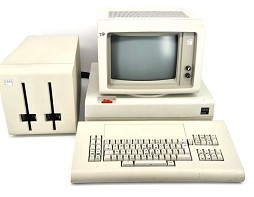
\includegraphics{~/GitHub/AGFA-LN-POS/author-final/part-0/Apparaetle.jpg}
\end{center}
\vspace{.5cm}
%\vspace{\baselineskip}
\begin{flushright}\noindent
${}$\hfill {\it The authors} \\
\end{flushright}



%%%%%%%%%%%%%%%%%%%%%%%acknow.tex%%%%%%%%%%%%%%%%%%%%%%%%%%%%%%%%%%%%%%%%%
% sample acknowledgement chapter
%
% Use this file as a template for your own input.
%
%%%%%%%%%%%%%%%%%%%%%%%% Springer %%%%%%%%%%%%%%%%%%%%%%%%%%

\extrachap{Acknowledgements}

Use the template \emph{acknow.tex} together with the document class SVMono (monograph-type books) or SVMult (edited books) if you prefer to set your acknowledgement section as a separate chapter instead of including it as last part of your preface.


%%
\tableofcontents
%%
%

\chapter{Acronyms}

\begin{description}
\item[$E_{\mathbb{R}}$, $E_{\mathbb{C}} = E$] real, complex Banach lattice
\item[$E_{+}$] positive cone
\item[$E'$] dual
\item[$E^*$] semigroup dual
\item[$E_{F}^{T}$] F-product of E with respect to semigroup T
\item[$E_{F}$] F-product of E
\item[$E_{f}$] see C-I,4
\item[$(E,\phi)$] see C-I,4
\item[$E\otimes F$] tensor product
\item[$L(E)$] bounded linear operators on E
\item[$Z(E)$] center of E
\item[$E_{n}$] n-th Sobolev space
\item[$B(H)$] W*-algebra of bounded linear operators on H
\item[$S(M)$] state space of C*-algebra M
\item[$M_{+}$] positive cone of C*-algebra M
\item[$M_{*}$] predual
\item[$M^{sa}$] self-adjoint part
\item[$M_{n}$] C*-algebra of nxn-matrices
\item[AC] absolutely continuous functions
\item[BV] functions of bounded variation
\item[K] compact topological space
\item[X] locally compact topological space
\item[$C(K)$, $C(K,E)$] continuous functions (with values in E)
\item[$C_{o}(X)$, $C_{o}(X,E)$] continuous functions vanishing at infinity with values in E
\item[$C^{b}(X)$] bounded continuous functions
\item[$C_{uu}(X)$] uniformly continuous functions
\item[$C^{n}$, $C^{(n)}$] continuous differentiable functions (n-times)
\item[$C_{c}^{\infty}(\mathbb{R}^n)$] infinitely differentiable functions with compact support
\item[$L^{p}(\mu)$] p-integrable functions
\item[$S(\mathbb{R}^n)$] Schwartz space
\item[$M(K)$] regular Borel measures
\item[$M_{b}(X)$] bounded regular Borel measures
\item[$T = (T(t))_{t\geq0}$] (one-parameter) semigroup
\item[$T|$] subspace (reduced) semigroup
\item[$T/$] quotient semigroup
\item[Fix$(T)$] fixed space of T
\item[$A$] generator
\item[$A'$] adjoint
\item[$A^*$] adjoint generator
\item[$\sigma(A)$] spectrum
\item[$\rho(A)$] resolvent set
\item[$\sigma_{ess}(A)$] essential spectrum
\item[$\sigma_{b}(A)$] boundary spectrum
\item[$P\sigma(A)$] point spectrum
\item[$P\sigma_{b}(A)$] boundary point spectrum
\item[$A\sigma(A)$] approximate point spectrum
\item[$R\sigma(A)$] residual spectrum
\item[$\omega = \omega(A) = \omega(T)$] growth bound
\item[$s(A)$] spectral bound
\item[$\omega_{I}(A)$] growth bound of solution of (ACP)
\item[$\omega(f)$] growth bound of $T(\cdot)f$
\item[$r(T)$] spectral radius
\item[$\omega_{ess}(A)$] essential growth bound
\item[$r_{ess}(T)$] essential spectral radius
\item[$R(\lambda,A)$] resolvent operator
\item[$I^{d}$, $\{I^{d}\}_{d=1}^{dd}$] orthogonal band of I (of $I^{d}$)
\item[$\wedge$] infimum
\item[$\vee$] supremum
\item[$|T|$] modulus of regular operator
\item[$\hat{f}$, $\check{f}$] Fourier (inverse Fourier) transformation
\item[$d\rho(f)$] subdifferential of $\rho$ in f
\item[$dN(f)$] subdifferential of norm in f
\item[$dN^{+}(f)$] subdifferential of canonical half-norm in f
\item[im] range
\item[ker] null-space
\item[Im] imaginary part
\item[Re] real part
\item[$\text{Re}f$, $\text{Im}f$] see C-I,7
\item[$\text{Re}T$, $\text{Im}T$] see C-I,7
\item[$\bar{f}$] complex conjugate of f
\item[$S_{f}$] signum operator with respect to f
\item[sign $f$] signum of f
\item[$f^{[n]}$] see C-II,2.2
\item[$|f|$] absolute value of f
\item[$f^{+}$] positive part of f
\item[$f^{-}$] negative part of f
\item[Id] identity operator
\item[$M_{p}$] multiplication operator
\item[1] function identically 1
\item[$1_{C}$] characteristic function of set C
\item[$\delta_{x}$] Dirac measure in x
\item[tr] trace
\item[span M] linear subspace generated by M
\item[$S(\alpha)$] sector in complex plane
\item[(ACP)] abstract Cauchy problem
\item[(P)] positive minimum principle
\item[(P')] B-II,1.21
\item[(K)] Kato's (equality) inequality
\item[(RCP)] retarded Cauchy problem
\item[(RE)] retarded equation
\item[(T)] translation property
\end{description}
%%
%%
%\mainmatter%%%%%%%%%%%%%%%%%%%%%%%%%%%%%%%%%%%%%%%%%%%%%%%%%%%%%%%
%
%%% -- Part-A
% !TEX root = ../../LN-Book.tex
%% -- Stand 2025/01/13
%% -- ulgr
%% -- Part A
%% --

\begin{partbacktext}
\part[One-parameter Semigroups on Banach Spaces]{One-parameter Semigroups on \\Banach Spaces }
\end{partbacktext}
% !TEX root = ../../LN-Book.tex
%% -- Stand 2025/01/18
%% -- ulgr
%% --

\chapter{Basic Results on Semigroups on Banach Spaces}\label{chap:A-I}
%% --
Since the basic theory of one-parameter semigroups can be found in several excellent books (e.g. Davies (1980), Goldstein (1985a), Pazy (1983) or Hille-Phillips (1957)) we do not want to give a self-contained introduction to this subject here.
It may however be useful to fix our notation, to collect briefly some important definitions and results (Section 1), to present a list of standard examples (Section 2) and to discuss standard constructions of new semigroups from a given one (Section 3).
In the entire chapter we denote by $E$ a (real or) complex Banach space and consider one-parameter semigroups of bounded linear operators $T(t)$ on $E$.
By this we understand a subset $\{T(t) \colon t \in \mathbb{R}_{+}\}$ of $L(E)$, usually written as $(T(t))_{t \geq 0}$, such that
%% --
\begin{align*}
	T(0) 	&= 	Id \\
	T(s+t) 	&= 	T(s) \cdot T(t) \text{ for all $s, t \in \mathbb{R}_{+}$.}
\end{align*}
%% --
In more abstract terms this means that the map $t \mapsto T(t)$ is a homomorphism from the additive semigroup $\mathbb{R}_{+}$ into the multiplicative semigroup $(L(E), \cdot)$.
Similarly, a one-parameter group $(T(t))_{t \in \mathbb{R}}$ will be a homomorphic image of the group $(\mathbb{R},+)$ in $(L(E), \cdot)$.
%% --
\section{Standard Definitions and Results}
%% --
We consider a one-parameter semigroup $(T(t))_{t \geq 0}$ on a Banach space $E$ and observe that the domain $\mathbb{R}_{+}$ and the range $L(E)$ of the (semigroup) homomorphism $\tau \colon t \mapsto T(t)$ are topological semigroups for the natural topology on $\mathbb{R}_{+}$ and any one of the standard operator topologies on $L(E)$.
We single out the strong operator topology on $L(E)$ and require $\tau$ to be continuous.
%% --
\begin{definition}
A one-parameter semigroup $(T(t))_{t \geq 0}$ is called strongly continuous if the map $t \mapsto T(t)$ is continuous for the strong operator topology on $L(E)$, i.e., $\lim_{t \to t_0} \|T(t)f - T(t_0)f\| = 0$ for every $f \in E$ and $t, t_0 \geq 0$.
\end{definition}
%% --
Clearly one defines in a similar way weakly continuous, resp. uniformly continuous (compare A-II, Def. 1.19) semigroups, but since we concentrate on the strongly continuous case we agree on the following terminology:
From now on \enquote*{semigroup} always means strongly continuous one-parameter semigroup of bounded linear operators.

Next we collect a few elementary facts on the continuity and boundedness of one-parameter semigroups.
%% --
\begin{remark}
%% --
\begin{enumerate}[(i)]
\item
A one-parameter semigroup $(T(t))_{t \geq 0}$ on a Banach space $E$ is strongly continuous if and only if for any $f \in E$ it is true that $T(t)f \to f$ as $t \to 0$.

\item
For every strongly continuous semigroup $(T(t))_{t \geq 0}$ there exist constants $M \geq 1$, $\omega \in \mathbb{R}$ such that $\|T(t)\| \leq M \cdot e^{\omega t}$ for every $t \geq 0$.

\item
If $(T(t))_{t \geq 0}$ is a one-parameter semigroup such that $\|T(t)\|$ is bounded for $0 \leq t \leq \delta$ then it is strongly continuous if and only if $\lim_{t \to 0} T(t)f = f$ for every $f$ in a total subset of $E$.

\end{enumerate}
%% --
\end{remark}
%% --
\begin{definition}
By the growth bound (or type) of the semigroup $(T(t))_{t \geq 0}$ we understand the number
%% --
\begin{align*}
\omega_{0} &:= \inf\{w \in \mathbb{R} \colon \text{There exists $ M \in \mathbb{R}_{+}$ such that $\|T(t)\| \leq M e^{wt}$ 
	for $t \geq 0$} \} \tag{*}\\
&= \lim_{t \to \infty} \frac{1}{t} \cdot \log\|T(t)\| = \inf_{t > 0} \frac{1}{t} \cdot \log\|T(t)\|
\end{align*}
\end{definition}
%% --
Particularly important are semigroups such that for every $t \geq 0$ we have $\|T(t)\| \leq M$ (bounded semigroups) or $\|T(t)\| \leq 1$ (contraction semigroups).
In both cases we have $\omega_{0} \leq 0$.

It follows from the subsequent examples and from 3.1 that $\omega_{0}$ may be any number $-\infty \leq \omega_{0} < +\infty$.
Moreover the reader should observe that the infimum in $ (*) $ need not be attained and that $M$ may be larger than $ 1 $ even for bounded semigroups.
%% --
\begin{example}
\begin{enumerate}[(i)]
\item
Take $E = \mathbb{C}^{2}$, $A = \begin{pmatrix} 0 & 1 \\ 0 & 0 \end{pmatrix}$ and $T(t) = e^{tA} = \begin{pmatrix} 1 & t \\ 0 & 1 \end{pmatrix}$.
Then for the $1$-norm on $E$ we obtain $\|T(t)\| = 1 + t$, hence $(T(t))_{t \geq 0}$ is an unbounded semigroup having growth bound $\omega_{0} = 0$.

\item
Take $E = L^{1}(\mathbb{R})$ and for $f \in E$ and $t \geq 0$ define
%% --
\[
	T(t)f(x) := \begin{cases}
		2 \cdot f(x+t) & \text{if } x \in [-t,0] \\
		f(x+t) & \text{otherwise.}
\end{cases}
\]
%% --
Each $T(t)$, $t > 0$, satisfies $\|T(t)\| = 2$ as can be seen by taking $f := 1_{[0,t]}$.
Therefore $(T(t))_{t \geq 0}$ is a strongly continuous semigroup which is bounded, hence has $\omega_{0} = 0$, but the constant $M$ in $ (*) $ cannot be chosen to be $ 1 $.

\end{enumerate}
\end{example}
%% --
\begin{definition}
To every semigroup $(T(t))_{t \geq 0}$ there belongs an operator $(A,D(A))$, called the generator and defined on the domain
\[
D(A) := \left\{f \in E \colon \lim_{h \to 0} \frac{T(h)f-f}{h} \text{ exists in } E\right\}
\]
by $Af := \lim_{h \to 0} \frac{T(h)f-f}{h}$ for $f \in D(A)$.
\end{definition}
%% --
Clearly, $D(A)$ is a linear subspace of $E$ and $A$ is linear from $D(A)$ into $E$.
Only in certain special cases (see 2.1) the generator is everywhere defined and therefore bounded (use Prop. 1.9(i)).
In general the precise extent of the domain $D(A)$ is essential for the characterisation of the generator.
But since the domain is canonically associated to the generator of a semigroup we shall write in most cases $A$ instead of $(A,D(A))$.
%% --
\begin{proposition}
For the generator $A$ of a semigroup $(T(t))_{t \geq 0}$ on a Banach space $E$ the following assertions hold:

\begin{enumerate}[(i)]
\item
If $f \in D(A)$ then $T(t)f \in D(A)$ for every $t \geq 0$.

\item
The map $t \mapsto T(t)f$ is differentiable on $\mathbb{R}_{+}$ if and only if $f \in D(A)$.
In that case one has
%% --
\begin{equation}
\frac{d}{dt}T(t)f = AT(t)f = T(t)Af.
\end{equation}
%% --
\item
Every $f \in E$ one has $\int_0^{t} T(s)f ds \in D(A)$ and
%% --
\begin{equation}
A\int_0^{t} T(s)f ds = T(t)f - f.
\end{equation}
%% --
\item
If $f \in D(A)$ then
%% --
\[
T(t)f = f + \int_0^{t} AT(s)f ds = f + \int_0^{t} T(s)Af ds.
\]
%% --
\item
The domain $D(A)$ is dense in $E$.

\end{enumerate}
\end{proposition}
%% --
\begin{theorem}
Let $(A,D(A))$ be the generator of a strongly continuous semigroup $(T(t))_{t \geq 0}$ on the Banach space $E$.
Then the \enquote*{abstract Cauchy problem} (ACP)
%% --
\[
\frac{d}{dt}\xi(t) = A\xi(t), \quad \xi(0) = f_0,
\]
has a unique solution $\xi \colon \mathbb{R}_{+} \to D(A)$ in $C^{1}(\mathbb{R}_{+},E)$ for every $f_0 \in D(A)$.
In fact, this solution is given by $\xi(t) := T(t)f_0$.
\end{theorem}
%% --
For the important relation of semigroups to abstract Cauchy problems we refer to A-II, Section 1.
Here we only point out that the above theorem implies that a semigroup is uniquely determined by its generator.
While the generator is bounded only for uniformly continuous semigroups (see 2.1 below), it always enjoys a weaker but useful property.
%% --
\begin{definition}
An operator $B$ with domain $D(B)$ on a Banach space $E$ is called closed if $D(B)$ endowed with the graph norm
\[
\|f\|_{B} := \|f\| + \|Bf\|
\]
becomes a Banach space.
Equivalently, $(B,D(B))$ is closed if and only if its graph $\{(f,Bf) \colon f \in D(B)\}$ is closed in $E \times E$, i.e.
\begin{equation}
f_{n} \in D(B), f_{n} \to f \text{ and } Bf_{n} \to g \text{ implies } f \in D(B) \text{ and } Bf = g.
\end{equation}
\end{definition}
%% --
It is clear from this definition that the \enquote*{closedness} of an operator $B$ depends very much on the size of the domain $D(B)$.
For example, a bounded and densely defined operator $(B,D(B))$ is closed if and only if $D(B) = E$.
On the other hand it may happen that $(B,D(B))$ is not closed but has a closed extension $(C,D(C))$, i.e., $D(B) \subset D(C)$ and $Bf = Cf$ for every $f \in D(B)$.
In that case, $B$ is called closable, a property which is equivalent to the following:
%% --
\begin{equation}
f_{n} \in D(B), f_{n} \to 0 \text{ and } Bf_{n} \to g \text{ implies } g = 0.
\end{equation}
%% --
The smallest closed extension of $(B,D(B))$ will be called the closure $\bar{B}$ with domain $D(\bar{B})$.
In other words, the graph of $\bar{B}$ is the closure of $\{(f,Bf) \colon f \in D(B)\}$ in $E \times E$.
Finally we call a subset $D_0$ of $D(B)$ a core for $B$ if $D_0$ is $\|\cdot\|_{B}$-dense in $D(B)$.
This means that a closed operator is determined (via closure) by its restriction to a core in its domain.
%% --
\begin{proposition}
For the generator $A$ of a strongly continuous semigroup $(T(t))_{t \geq 0}$ the following holds:

\begin{enumerate}[(i)]
\item
The generator $A$ is a closed operator.

\item
If a subspace $D_0$ of the domain $D(A)$ is dense in $E$ and $(T(t))$-invariant, then it is a core for $A$.
\item
Define $D(A^{n}) := \{f \in D(A^{n-1}) \colon Af \in D(A^{n-1})\}$, $D(A^{1}) = D(A)$.
Then $D(A^\infty) := \bigcap_{n \in \mathbb{N}} D(A^{n})$ is dense in $E$ and a core for $A$.

\end{enumerate}
\end{proposition}
%% --
\begin{example}
Property (iii) above does not hold for general densely defined closed operators.
Take $E = C[0,1]$, $D(B) = C^{1}[0,1]$ and $Bf = q \cdot f$ for some nowhere differentiable function $q \in C[0,1]$.
Then $B$ is closed, but $D(B^{2}) = (0)$.
\end{example}
%% --
\begin{proposition}
For the generator $A$ of a strongly continuous semigroup $(T(t))_{t \geq 0}$ on a Banach space $E$ the following holds.
If $\int_0^\infty e^{-\lambda t}T(t)f dt$ exists for every $f \in E$ and some $\lambda \in \mathbb{C}$, then $\lambda \in \rho(A)$ and $R(\lambda,A)f = \int_0^\infty e^{-\lambda t}T(t)f dt$.
In particular,
\begin{equation}
R(\lambda,A)^{n+1}f = \frac{(-1)^{n}}{n!}\left(\frac{d}{d\lambda}\right)^{n} R(\lambda,A)f = \int_0^\infty e^{-\lambda t}\frac{t^{n}}{n!}T(t)f dt
\end{equation}
for $n \in \mathbb{N}$, $f \in E$ and all $\lambda$ with $\operatorname{Re}\lambda > \omega$.
\end{proposition}
%% --
\begin{remark}

\begin{enumerate}[(i)]

\item
For continuous Banach space valued functions such as $t \mapsto T(t)f$ we consider the Riemann integral and define $\int_0^\infty T(t)f dt$ as $\lim_{t \to \infty} \int_0^{t} T(s)f ds$.
Sometimes such integrals for strongly continuous semigroups $(T(t))_{t \geq 0}$ are written as $\int_{a}^{b} T(t)dt$ and understood in the strong sense.

\item Since the generator $(A,D(A))$ determines the semigroup $(T(t))_{t > 0}$ uniquely, we will speak occasionally of the growth bound of the generator instead of the semigroup, i.e., we write $\omega = \omega(A) = \omega((T(t))_{t \geq 0})$.

\item
For one-parameter groups it might seem to be more natural to define the generator as the `derivative' rather than just the `right derivative' at $t = 0$.
This yields the same operator as the following result shows:
The strongly continuous semigroup $(T(t))_{t \geq 0}$ with generator $A$ can be extended to a strongly continuous one-parameter group $(U(t))_{t \in \mathbb{R}}$ if and only if $-A$ generates a semigroup $(S(t))_{t \geq 0}$.
In that case $(U(t))_{t \in \mathbb{R}}$ is obtained as
\[
U(t) := \begin{cases}
T(t) & \text{for } t \geq 0 \\
S(-t) & \text{for } t \leq 0
\end{cases}
\]
We refer to [Davies (1980), Prop.~1.14] for the details.

\end{enumerate}
\end{remark}

%% --
\section{Standard Examples}
In this section we list and discuss briefly the most basic examples of semigroups together with their generators.
These semigroups will reappear throughout this book and will be used to illustrate the theory.
We start with the class of semigroups mentioned after Definition 1.1.
%% --
\subsection{Uniformly Continuous Semigroups}
It follows from elementary operator theory that for every bounded operator $A \in L(E)$ the sum exists and determines a unique uniformly continuous (semi)group $(e^{tA})_{t \in \mathbb{R}}$ having $A$ as its generator.
%% --
\[
\sum_{n=0}^{m} \frac{t^n A^n}{n!} = \colon e^{tA}
\]
%% --
Conversely, any uniformly continuous semigroup is of this form: If the semigroup $(T(t))_{t \geq 0}$ is uniformly continuous, then $\frac{1}{t} \int_{0}^{t} T(s) ds$ uniformly converges to $T(0)=Id$ as $t \rightarrow 0$.
Therefore for some $t' \neq 0$ the operator $\frac{1}{t} \int_{0}^{t} T(s) ds$ is invertible and every $f \in E$ is of the form $f=\frac{1}{t} \int_{0}^{t'} T(s) g ds$ for some $g \in E$.
But these elements belong to $D(A)$ by (1.3), hence $D(A)=E$.
Since the generator $A$ is closed and everywhere defined it must be bounded.
Remark that bounded operators are always generators of groups, not just semigroups.
Moreover the growth bound $\omega$ satisfies $|\omega| \leq \|A\|$ in this situation.

The above characterization of the generators of uniformly continuous semigroups as the bounded operators shows that these semigroups are - at least in many aspects - rather simple objects.
%% --
\subsection{Matrix Semigroups}
The above considerations especially apply in the situation $E=\mathbb{C}^n$.
If $n=2$ and $A=(a_{ij})_{2\times 2}$ the following explicit formulas for $e^{tA}$ might be of interest:
Set $s:=\text{trace }A$, $d:=\text{det }A$ and $D:=(s^2-4d)^{1/2}$.
Then
%% --
\[
e^{tA}  = 
e^{ts/2} \cdot [D^{-1} 2\sinh(tD/2) \cdot A + (\cosh(tD/2)-sD^{-1}\sinh(tD/2)) \cdot Id]
\]
%% --
if $D \neq 0$ and
%% -- 
\[
e^{tA}  = 
e^{ts/2} \cdot [tA+(1-ts/2) \cdot Id] \text{\phantom{xxxxxxxxx}}
\]
%% --
if $D=\emptyset$ resp.
%% --
\subsection{Multiplication Semigroups}
Many Banach spaces appearing in applications are Banach spaces of (real or) complex valued functions over a set $X$.
As the most standard of these "function spaces", we mention the space $C_0(X)$ of all continuous complex valued functions vanishing at infinity on a locally compact space $X$, or the space $L^p(X,\Sigma,\mu), 1 \leq p \leq \infty$, of all (equivalence classes of) p-integrable functions on a $\sigma$-finite measure space $(X,\Sigma,\mu)$.

On these function spaces $E=C_0(X)$, resp. $E=L^p(X,\Sigma,\mu)$, there is a simple way to define \enquote{multiplication operators}: Take a continuous, resp. measurable function $q \colon X \rightarrow \mathbb{C}$ and define
%% --
\[
M_{q}f := q \cdot f, \text{ i.e. } M_{q}f(x) := q(x) \cdot f(x) \text{ for } x \in X,
\]
%% --
for every $f$ in the "maximal" domain $D(M_{q}) := \{g \in E \colon q \cdot g \in E\}$.

For such multiplication operators many properties can be checked quite directly.
For example, the following statements are equivalent:

\begin{enumerate}[(a)]
\item
$M_{q}$ is bounded.

\item
$q$ is (p-essentially) bounded.

\end{enumerate}
%% --
One has $\|M_{q}\| = \|q\|_\infty$ in this situation.

Observe that on spaces $C(K)$, $K$ compact, there are no densely defined, unbounded multiplication operators.

By defining the multiplication semigroups
%% --
\[
T(t)f(x) := \exp(t \cdot q(x))f(x), x \in X, f \in E,
\]
%% --
one obtains the following characterizations.

\begin{proposition} 
Let $M_{q}$ be a multiplication operator on $E=C_0(X)$ or $E=L^p(X,\Sigma,\mu), 1 \leq p < \infty$.
Then the properties (a) and (b), resp. $(a')$ and $(b')$, are equivalent:
\begin{enumerate}[(a)]
\item
$M_{q}$ generates a strongly continuous semigroup.
\item
$\sup\{\text{Re }q(x) \colon x \in X\} < \infty$.
\end{enumerate}
%% --

\begin{enumerate}[($a'$)]
\item
$M_{q}$ generates a uniformly continuous semigroup.
\item
$\sup\{|q(x)| \colon x \in X\} < \infty$.
\end{enumerate}
%% --
\end{proposition} 
As a consequence one computes the growth bound of a multiplication semigroup as follows:
\[
\omega = \sup\{\text{Re }q(x) \colon x \in X\} \text{ in the case } E = C_0(X),
\]
\[
\omega = \text{ess-sup}\{\text{Re }q(x) \colon x \in X\} \text{ in the case } E = L^p(\mu).
\]
%% --
It is a nice exercise to characterize those multiplication operators which generate strongly continuous groups.

\subsection{Translation (Semi)Groups}
Let $E$ be one of the following function spaces $C_0(\mathbb{R}_+)$, $C_0(\mathbb{R})$ or $L^p(\mathbb{R}_+)$, $L^p(\mathbb{R})$ for $1 \leq p < \infty$.
Define $T(t)$ to be the (left) translation operator
%% --
\[
T(t)f(x) := f(x+t)
\]
%% --
for $x$,  $t \in \mathbb{R}_+$, resp. $x,t \in \mathbb{R}$ and $f \in E$.
Then $(T(t))_{t \geq 0}$ is a strongly continuous semigroup, resp. group of contractions on $E$ and its generator is the first derivative $\frac{d}{dx}$ with 'maximal' domain.
In order to be more precise we have to distinguish the cases $E=C_0$ and $E=L^p$:

\begin{enumerate}[(i)]

\item
The generator of the translation (semi)group on $E=C_0(\mathbb{R}_+)$ is
\[
Af := \frac{d}{dx}f = f',
\]
with domain 
\[
D(A) := \{f \in E \colon f \text{ differentiable and } f' \in E\}
\]
%% --
\begin{proof} For $f \in D(A)$ it follows that for every $x \in \mathbb{R}_{(+)}$
\[
\lim_{h \to 0} \frac{T(h)f(x)-f(x)}{h} = \lim_{h \to 0} \frac{f(x+h)-f(x)}{h} \text{ exists}
\]
%% --
(uniformly in $x$) and coincides with $Af(x)$.
Therefore $f$ is differentiable and $f' \in E$.
On the other hand, take $f \in E$ differentiable such that $f' \in E$.
Then
\[
\left|\frac{f(x+h)-f(x)}{h}-f'(x)\right| \leq \frac{1}{h} \int_{x}^{x+h}|f'(y)-f'(x)| dy
\]
%% --
where the last expression tends to zero uniformly in $x$ as $h \to 0$.
Thus $f \in D(A)$ and $f' = Af$.
\end{proof}

\item 
The generator of the translation (semi)group on $E=L^p(\mathbb{R}_{(+)}), 1 \leq p < \infty$, is
\[
Af := \frac{d}{dx}f = f',
\]
with domain
\[
D(A) := \{f \in E \colon f \text{ absolutely continuous}, f' \in E\}
\]
\end{enumerate}
%% --
\subsection{Rotation Groups}
On $E=C(\mathbb{T})$, resp. $E=L^p(\mathbb{T},m), 1 \leq p < \infty$, $m$ Lebesgue measure we have canonical groups defined by rotations of the unit circle $\mathbb{T}$ with a certain period.
For $0 < \tau \in \mathbb{R}$ the operators
%% --
\[
R_\tau(t)f(z) := f(e^{2\pi it/\tau} \cdot z)
\]
%% --
yield a group $(R_\tau(t))_{t \in \mathbb{R}}$ having period $\tau$, i.e. $R_\tau(\tau)=Id$.
As in Example 2.4 one shows that its generator has the form
%% --
\[
D(A) = \{f \in E \colon f \text{ absolutely continuous}, f' \in E\},
\]
\[
Af(z) = (2\pi i/\tau) \cdot z \cdot f'(z).
\]
%% --
An isomorphic copy of the group $(R_\tau(t))_{t \in \mathbb{R}}$ is obtained if we consider $E=\{f \in C[0,1] \colon f(0)=f(1)\}$, resp. $E=L^p([0,1])$ and the group of 'periodic translations'
%% --
\[
T(t)f(x) := f(y) \text{ for } y \in [0,1], y = x+t \text{ mod } 1
\]
%% --
with generator
%% --
\[
D(A) := \{f \in E \colon f \text{ absolutely continuous}, f' \in E\},
\]
\[
Af := f'.
\]
%% --
\subsection{Nilpotent Translation Semigroups}
Take $E=L^p([0,\tau],m)$ for $1 \leq p < \infty$ and define
%% --
\[
T(t)f(x) := \begin{cases}
f(x+t) & \text{if } x+t \leq \tau \\
0 & \text{otherwise}
\end{cases}
\]
%% --
Then $(T(t))_{t \geq 0}$ is a semigroup satisfying $T(t)=0$ for $t \geq \tau$.
Its generator is still the first derivative $A=\frac{d}{dx}$, but its domain is
\[
D(A) = \{f \in L^p([0,\tau]) \colon f \text{ absolutely continuous}, f' \in L^p([0,\tau]), f(\tau)=0\}.
\]
%% --
In fact, if $f \in D(A)$ then $f$ is absolutely continuous with $f' \in E$.
By Prop.1.6.i it follows that $T(t)f$ is absolutely continuous and hence $f(\tau)=0$.
%% --
\subsection{One-dimensional Diffusion Semigroup}
For the second derivative
%% --
\[
Bf(x) := \frac{d^2}{dx^2}f(x) = f''(x)
\]
%% --
we take the domain
\[
D(B) := \{f \in C^2[0,1] \colon f'(0)=f'(1)=0\}
\]
in the Banach space $E=C[0,1]$.
Then $D(B)$ is dense in $C[0,1]$, but closed for the graph norm.
Obviously, each function
%% --
\[
e_{n}(x) := \cos \pi nx, \quad n \in \mathbb{Z},
\]
%% --
is contained in $D(B)$ and an eigenfunction of $B$ pertaining to the eigenvalue $\lambda_{n} := -\pi^2n^2$.
The linear hull
\[
\text{span}\{e_{n} \colon n \in \mathbb{Z}\} = \colon E_0
\]
forms a subalgebra of $D(B)$ which by the Stone-Weierstrass theorem is dense in $E$.

We now use $e_{n}$ to define bounded linear operators
\[
e_{n} \otimes e_{n} \colon f \rightarrow \left(\int_0^1 f(x)e_{n}(x)dx\right)e_{n} = \langle f,e_{n}\rangle e_{n}
\]
satisfying $\|e_{n} \otimes e_{n}\| \leq 1$ and
$(e_{n} \otimes e_{n})(e_{m} \otimes e_{m}) = \delta_{n,m}(e_{n} \otimes e_{n})$ for $n \in \mathbb{Z}$.

For $t>0$ we define
\[
\begin{aligned}
T(t) &:= \sum_{n \in \mathbb{Z}} \exp(-\pi^2n^2t) \cdot e_{n} \otimes e_{n} \\
&= e_0 \otimes e_0 + 2\sum_{n=1}^{\infty} \exp(-\pi^2n^2t) \cdot e_{n} \otimes e_{n}
\end{aligned}
\]
%% --
or
%% --
\[
\begin{aligned}
T(t)f(x) &= \int_0^1 k_{t}(x,y)f(y)dy \\
&\text{where } k_{t}(x,y) = 1 + 2\sum_{n=1}^{\infty} \exp(-\pi^2n^2t)\cos \pi nx \cos \pi ny.
\end{aligned}
\]
%% --
Die Jacobi-Identität
\[
\begin{aligned}
w_{t}(x) &:= 1/(4\pi t)^{\frac{1}{2}} \sum_{m \in \mathbb{Z}} \exp(-(x+2m)^2/4t) \\
&= \frac{1}{2} + \sum_{n \in \mathbb{N}} \exp(-\pi^2n^2t)\cos \pi nx
\end{aligned}
\]
%% --
und trigonometrische Beziehungen zeigen, dass
\[
k_{t}(x,y) = w_{t}(x+y) + w_{t}(x-y)
\]
%% --
welches eine positive Funktion auf $[0,1]^2$ ist.
Daher ist $T(t)$ ein beschränkter Operator auf $C[0,1]$ mit
\[
\|T(t)\| = \|T(t)1\| = \sup_{x \in [0,1]} \int_0^1 k_{t}(x,y)dy = 1.
\]
%% --
\subsection{n-dimensional Diffusion Semigroup}
On $E=L^p(\mathbb{R}^n), 1 \leq p < \infty$, the operators
%% --
\[
\begin{aligned}
T(t)f(x) &:= (4\pi t)^{-n/2} \int_{\mathbb{R}^n} \exp(-|x-y|^2/4t)f(y)dy \\
&:= \psi_{t} * f(x)
\end{aligned}
\]
%% --
for $x \in \mathbb{R}^n$, $t>0$ and $\psi_{t}(x) := (4\pi t)^{-n/2}\exp(-|x|^2/4t)$ form a strongly continuous semigroup.

In fact the integral exists for every $f \in L^p(\mathbb{R}^n)$, since $\psi_{t}$ is an element of the Schwartz space $\mathcal{S}(\mathbb{R}^n)$ of all rapidly decreasing smooth functions on $\mathbb{R}^n$.

Moreover,
\[
\|T(t)f\|_{p} \leq \|\psi_{t}\|_{1}\|f\|_{p} = \|f\|_{p}
\]
%% --
by Young's inequality [Reed-Simon (1975), p.28], hence $\|T(t)\| \leq 1$ for every $t>0$.

Next we observe that $\mathcal{S}(\mathbb{R}^n)$ is dense in $E$ and invariant under each $T(t)$.
Therefore we can apply the Fourier transformation $\mathcal{F}$ which leaves $\mathcal{S}(\mathbb{R}^n)$ invariant and yields
\[
\mathcal{F}(\psi_{t} * f) = (2\pi)^{n/2}\mathcal{F}(\psi_{t}) \cdot \mathcal{F}(f) = (2\pi)^{n/2}\hat{\psi_{t}} \cdot \hat{f}
\]
where $f \in \mathcal{S}(\mathbb{R}^n)$, $\hat{f} = \mathcal{F}f \in \mathcal{S}(\mathbb{R}^n)$.

In other words, $\mathcal{F}$ transforms $(T(t)|_{\mathcal{S}(\mathbb{R}^n)})_{t \geq 0}$ into a multiplication semigroup on $\mathcal{S}(\mathbb{R}^n)$ which is pointwise continuous for the usual topology of $\mathcal{S}(\mathbb{R}^n)$.
The generator, i.e. the right derivative at 0, of this semigroup is the multiplication operator
\[
B\hat{f}(x) := -|x|^2\hat{f}(x)
\]
for every $f \in \mathcal{S}(\mathbb{R}^n)$.

Applying the inverse Fourier transformation and observing that the topology of $\mathcal{S}(\mathbb{R}^n)$ is finer than the topology induced from $L^p(\mathbb{R}^n)$, we obtain that $(T(t))_{t \geq 0}$ is a semigroup which is strongly continuous (use Remark 1.2, (3)) and its generator $A$ coincides with
\[
\Delta f(x) = \sum_{i=1}^n \frac{\partial^2}{\partial x_{i}^2}f(x_{1},\ldots,x_{n})
\]
for every $f \in \mathcal{S}(\mathbb{R}^n)$.

Since $\mathcal{S}(\mathbb{R}^n)$ is $(T(t))$-invariant we have determined the generator on a core of its domain (see Prop.1.9.ii).

In particular the above semigroup 'solves' the initial value problem for the \enquote{heat equation}
%% --
\[
\frac{\partial}{\partial t}f(x,t) = \Delta f(x,t), \quad f(x,0) = f_0(x), \quad x \in \mathbb{R}^n.
\]
%% --
For the analogous discussion of the unitary group on $L^2(\mathbb{R}^n)$ generated by
$ $  -- $ $
\[
C := i\Delta
\]
we refer to Section IX.7 in Reed-Simon (1975).
%% --
\section{Standard Constructions}
Starting with a semigroup $(T(t))_{t \geq 0}$ on a Banach space $E$ it is possible to construct new semigroups on spaces naturally associated with $E$.
Such constructions will be important technical devices in many of the subsequent proofs.
Although most of these constructions are rather routine, we present in the sequel a systematic account of them for the convenience of the reader.

We always start with a semigroup $(T(t))_{t \geq 0}$ on a Banach space $E$, and denote its generator by $A$ on the domain $D(A)$.

\subsection{Similar Semigroups}
There is an easy way how to obtain different (but isomorphic) semigroups: Take any isomorphism $S \in L(E,F)$ between two Banach spaces $E$ and $F$.
Then
\[
U(t) := ST(t)S^{-1}, \quad t \geq 0,
\]
defines a semigroup on $F$ which is strongly continuous if and only if $(T(t))_{t \geq 0}$ has this property.
In this case the generator $B$ of $(U(t))_{t \geq 0}$ is given by
\[
B = SAS^{-1} \text{ with } D(B) = SD(A).
\]

%% -- Chapter A-II
%% --

\chapter{Characterization of Semigroups on Banach Spaces}\label{chap:A-II}

In this chapter two different problems are treated:

\begin{enumerate}[(i)]
\item to characterize generators of strongly continuous semigroups;
\item to characterize various properties of strongly continuous semigroups in terms of their generators.
\end{enumerate}

In Section 1 the first problem is solved by finding conditions on the Cauchy problem associated with $A$ and also by finding conditions on the resolvent of $A$.
The second problem is treated for a hierarchy of smoothness properties of the semigroup.

Contraction semigroups are considered in Section 2.
Here, the first problem has a simple and extremely useful solution: A densely defined operator $A$ is generator of a contraction semigroup if and only if $A$ is dissipative and satisfies a range condition.

Our approach is quite general.
We do not only consider contractions with respect to the norm but also with respect to \enquote{half-norms}.
This will allow us to obtain results on positive contraction semigroups simultaneously by choosing a suitable half-norm (cf.\ C-II,Sec.1).

The last section contains a surprising result: on certain Banach spaces (e.g., $L^{\infty}$) only bounded operators are generators of strongly continuous semigroups.

\section{The Abstract Cauchy Problem, Special Semigroups and Perturbation}

Linear differential equations in Banach spaces are intimately connected with the theory of one-parameter semigroups.
In fact, given a closed linear operator $A$ with dense domain $D(A)$ the following statement is true (with some reservation regarding a technical detail): The abstract Cauchy problem
%% -- 
\[
\begin{aligned}
\dot{u}(t) &= Au(t) \quad (t \geq 0) \\
u(0) &= f
\end{aligned}
\]
%% -- 
has a unique solution for every $f \in D(A)$ if and only if $A$ is the generator of a strongly continuous semigroup.

This is one characterization of generators which illustrates their important role for applications.
The fundamental Hille-Yosida theorem gives a different characterization in terms of the resolvent and yields a powerful tool for actually proving that a given operator is the generator of a semigroup.

Another problem we will treat here is how diverse properties of a semigroup can be described in terms of its generator.
This is a reasonable question from the theoretical point of view (since the generator uniquely determines the semigroup).
It is of interest from the practical point of view as well: the generator is the given object, defined by the differential equation.
It is useful to dispose of conditions of the generator itself giving information on the solutions (which might not be known explicitly).
We discuss smoothness properties such as analyticity, differentiability, norm continuity and compactness of the semigroup.

A frequent method to obtain new generators out of a given one is by perturbation.
We will have a brief look at this circle of problems at the end of this section.

The results are explained and illustrated by examples.
Proofs are only given when new aspects are presented which are not yet contained in the literature, otherwise we refer to the recent monographs Davies (1980), Goldstein (1985a), Pazy (1983).

% chapter-A-II-1-section1.tex

\subsection{The Abstract Cauchy Problem}\label{sec:acp}

Let $A$ be a closed operator on a Banach space $E$ and consider the abstract Cauchy problem
%% -- 
\[
\begin{aligned}
\text{(ACP)} \quad \begin{cases}
\dot{u}(t) &= Au(t) \quad (t \geq 0) \\
u(0) &= f.
\end{cases}
\end{aligned}
\]
%% -- 
By a solution of (ACP) for the initial value $f \in D(A)$ we understand a continuously differentiable function $u : [0,\infty) \to E$ satisfying $u(0) = f$ and $u(t) \in D(A)$ for all $t \geq 0$ such that $\dot{u}(t) = Au(t)$ for $t \geq 0$.

By A-I,Thm.1.7 there exists a unique solution of (ACP) for all initial values in the domain $D(A)$ whenever $A$ is the generator of a strongly continuous semigroup.
The converse does not hold (see Example 1.4.\ below).
However, for the operator $A_{1}$ on the Banach space $E_{1} = D(A)$ (see A-I,3.5) with domain $D(A_{1}) = D(A^{2})$ given by $A_{1}f = Af$ $(f \in D(A_{1}))$ the following holds.

\begin{theorem}\label{thm:1.1}
The following assertions are equivalent.
\begin{enumerate}[(a)]
\item For every $f \in D(A)$ there exists a unique solution of (ACP).
\item $A_{1}$ is the generator of a strongly continuous semigroup.
\end{enumerate}
\end{theorem}

\begin{proof}
(i) implies (ii).
Assume that (i) holds; i.e., for every $f \in D(A)$ there exists a unique solution $u(\cdot,f) \in C^{1}([0,\infty),E)$ of (ACP).
For $f \in E_{1}$ define $T_{1}(t)f := u(t,f)$ $(t\geq0)$.
By the uniqueness of the solutions it follows that $T_{1}(t)$ is a linear operator on $E_{1}$ and $T_{1}(s+t) = T_{1}(s)T_{1}(t)$.
Moreover, since $u(\cdot,f) \in C^{1}$, it follows that $t \mapsto T_{1}(t)f$ is continuous from $[0,\infty)$ into $E_{1}$.
We show that $T_{1}(t)$ is a continuous operator for all $t>0$.

Let $t>0$.
Consider the mapping $\eta: E_{1} \to C([0,t],E_{1})$ given by $\eta(f) = T_{1}(\cdot)f = u(\cdot,f)$.
We show that $\eta$ has a closed graph.
In fact, let $f_{n} \to f$ in $E_{1}$ and $\eta(f_{n}) = u(\cdot,f_{n}) \to v$ in $C([0,t],E_{1})$.
Then $u(s,f_{n}) = f_{n} + \int_0^s Au(r,f_{n})dr$.
Letting $n\to\infty$ we obtain $v(s) = f + \int_0^s Av(r)dr$ for $0 \leq s \leq t$.
Let $\tilde{v}(s) = T_{1}(s-t)v(t)$ for $s > t$, and $\tilde{v}(s) = v(s)$ for $0 \leq s \leq t$.
% continuation of chapter-A-II-1-section1.tex

Then $\tilde{v}$ is a solution of (ACP).
It follows that $\tilde{v}(s) = T_{1}(s)f$ for all $s \geq 0$.
Hence $v = \eta(f)$.
We have shown that $\eta$ has a closed graph and so $\eta$ is continuous.
This implies the continuity of $T_{1}(t)$.
It remains to show that $A_{1}$ is the generator of $(T_{1}(t))_{t\geq0}$.

We first show that for $f \in D(A^{2})$ one has
%% -- 
\[
AT_{1}(t)f = T_{1}(t)Af. \tag{1.1}
\]
%% -- 

In fact, let $v(t) = f + \int_{0}^{t} u(s,Af) ds$.
Then $\dot{v}(t) = u(t,Af) = Af + \int_{0}^{t} Au(s,Af) ds = A(f + \int_{0}^{t} u(s,Af) ds) = Av(t)$.
Since $v(0) = f$, it follows that $v(t) = u(t,f)$.
Hence $Au(t,f) = Av(t) = \dot{v}(t) = u(t,Af)$.
This is (1.1).

Now denote by $B$ the generator of $(T_{1}(t))_{t\geq0}$.
For $f \in D(A^{2})$ we have
%% -- 
\[
\lim_{t \to 0} \frac{T_{1}(t)f - f}{t} = Af
\]
%% -- 
and by (1.1),
%% -- 
\[
\lim_{t \to 0} A \frac{T_{1}(t)f - f}{t} = \lim_{t \to 0} \frac{T_{1}(t)Af - Af}{t} = A^{2}f \text{ in the norm of } E.
\]
%% -- 

Hence $\lim_{t \to 0} \frac{T_{1}(t)f - f}{t} = Af$ in the norm of $E_{1}$.

This shows that $A_{1} \subset B$.
In order to show the converse, let $f \in D(B)$.
Then $\lim_{t \to 0} A \frac{T_{1}(t)f - f}{t}$ exists in the norm of $E$.
Since $\lim_{t \to 0} \frac{T_{1}(t)f - f}{t} = Af$ in the norm of $E$, it follows that $Af \in D(A)$, since $A$ is closed.
Thus $f \in D(A^{2}) = D(A_{1})$.
We have shown that $B = A_{1}$.

(ii) implies (i).
Assume that $A_{1}$ is the generator of a strongly continuous semigroup $(T_{1}(t))_{t\geq0}$ on $E_{1}$.
Let $f \in D(A)$ and set $u(t) = T_{1}(t)f$.
Then $u \in C([0,\infty),E)$ and $Au(\cdot) \in C([0,\infty),E)$.
Moreover, $\int_{0}^{t} u(s)ds = \int_{0}^{t} T_{1}(s)fds \in D(A_{1}) = D(A^{2})$ and $A\int_{0}^{t} u(s)ds = u(t) - u(0) = u(t) - f$ (by A-I, (1.3)).
Consequently, $u(t) = f + A\int_{0}^{t} u(s)ds = f + \int_{0}^{t} Au(s)ds$.
Hence $u \in C^{1}([0,\infty),E)$ and $\dot{u}(t) = Au(t)$.
Thus $u$ is a solution of (ACP).

% continuation of chapter-A-II-1-section1.tex

In order to show uniqueness, assume that $u$ is a solution of (ACP) with initial value $0$.
We have to show that $u \equiv 0$.
Let $v(t) = \int_{0}^{t} u(s)ds$.
Then $v(t) \in D(A)$ and $Av(t) = \int_{0}^{t} Au(s)ds = \int_{0}^{t} \dot{u}(s)ds = u(t) \in D(A)$.
Consequently, $v(t) \in D(A^{2})$ for all $t\geq0$.
Moreover, $\dot{v}(t) = u(t) = Av(t)$ and $\frac{d}{dt} Av(t) = Au(t) = A\dot{v}(t) = A^{2}v(t)$.
Thus $v \in C^{1}([0,\infty),E_{1})$ and $\dot{v}(t) = A_{1}v(t)$.
Since $v(0) = 0$, it follows that $v \equiv 0$.
Thus $u \equiv v \equiv 0$.
\end{proof}

If (ACP) has a unique solution for every initial value in $D(A)$, then $A$ is the generator of a strongly continuous semigroup only if some additional assumptions on the solutions (continuous dependence from the initial value) or on $A$ $(\rho(A) \neq \emptyset)$ are made.

\begin{corollary}\label{cor:1.2}
Let $A$ be a closed operator.
Consider the following existence and uniqueness condition.

(EU) For every $f \in D(A)$ there exists a unique solution $u(\cdot,f)\in C^{1}([0,\infty),E)$ of the Cauchy problem associated with $A$ having the initial value $u(0,f) = f$.

The following assertions are equivalent.
\begin{enumerate}[(a)]
\item $A$ is the generator of a strongly continuous semigroup.
\item $A$ satisfies (EU) and $\rho(A) \neq \emptyset$.
\item $A$ satisfies (EU) and for every $\mu \in \mathbb{R}$ there exists $\lambda > \mu$ such that $(\lambda-A)D(A) = E$.
\item $A$ satisfies (EU), has dense domain and for every sequence $(f_{n})$ in $D(A)$ satisfying $\lim_{n \to \infty}f_{n} = 0$ one has $\lim_{n \to \infty}u(t,f_{n}) = 0$ uniformly in $t \in [0,1]$.
\end{enumerate}
\end{corollary}

\begin{proof}
It is clear that (i) implies the remaining assertions.
So assume that $A$ satisfy (EU).
Then by Theorem 1.1., $A_{1}$ is a generator.
If there exists $\lambda \in \rho(A)$, then $(\lambda-A)$ is an isomorphism from $E_{1}$ onto $E$ and $A$ is similar to $A_{1}$ via this isomorphism [since $D(A_{1}) = \{(\lambda-A)^{-1}f : f \in D(A)\}$ and $Af = (\lambda-A)A_{1}(\lambda-A)^{-1}f$ for all $f \in D(A)$, see A-I,3.0].
Thus $A$ is a generator on $E$ and we have shown that (ii) implies (i).

If (iii) holds, then there exists $\lambda > s(A_{1})$ such that $(\lambda-A)D(A) = E$.
We show that $(\lambda-A)$ is injective.
Then $\lambda \in \rho(A)$ since $A$ is closed.
Assume that $Af = \lambda f$ for some $f \in D(A)$.
Then $f \in D(A^{2}) = D(A_{1})$, and so $f = 0$ since $\lambda \in \rho(A_{1})$.
This proves that (iii) implies (ii).
We have shown existence.


It remains to show that (iv) implies (i).

Assertion (iv) implies that for all $t \geq 0$ there exist bounded operators $T(t) \in \mathcal{L}(E)$ such that $u(t,f) = T(t)f$ if $f \in D(A)$.
Moreover, $\sup_{0\leq t\leq1} \|T(t)\| < \infty$.
It follows that $T(\cdot)f$ is strongly continuous for all $f \in E$ (since it is so for $f \in D(A)$ and $D(A)$ is dense).
Let $t > 1$.
There exist unique $n \in \mathbb{N}$ and $s \in [0,1)$ such that $t = n + s$.
Let $T(t) := T(1)^{n}T(s)$.
From the uniqueness of the solutions it follows that $T(t)f = u(t,f)$ for all $t \geq 0$ as well as $T(t+s)f = T(s)T(t)f$ for all $f \in D(A)$ and $s,t \geq 0$.
Thus $(T(t))_{t\geq0}$ is a semigroup.
Denote by $B$ its generator.
It follows from the definition that $A \subset B$.
Moreover, $D(A)$ is invariant under the semigroup.
So by A-I,Prop.1.9.(ii) $D(A)$ is a core of $B$.
Since $A$ is closed this implies that $A = B$.
\end{proof}

\begin{remark}\label{rem:1.3}
It is surprising that from condition (ii) and (iii) in the corollary it follows automatically that $D(A)$ is dense.
On the other hand this condition cannot be omitted in (iv).
In fact, consider any generator $\tilde{A}$ and its restriction $A$ with domain $D(A) = \{0\}$.
Then $A$ satisfies the remaining conditions in (iv) but is not a generator (if $\dim E > 0$).
\end{remark}

\begin{example}\label{ex:1.4}
We give a densely defined closed operator $A$, such that there exists a unique solution of (ACP) for all initial values in $D(A)$, but $A$ is not a generator.
Let $B$ be a densely defined unbounded closed operator on a Banach space $F$.
Consider $E = F \oplus F$ and $A$ on $E$ given by
%% -- 
\[
A = \begin{pmatrix} 0 & B \\ 0 & 0 \end{pmatrix}
\]
%% -- 
with domain $F \times D(B)$.

Then $D(A^{2}) = \{(f,g) \in F \times D(B) : Bg \in F\} = D(A)$ and so $A_{1} \in \mathcal{L}(E_{1})$.
In particular, $A_{1}$ is a generator.
But $A$ is not.
For instance condition (ii) in Corollary 1.2.\ does not hold, since for each $\lambda \in \mathbb{C}$,
%% -- 
\[
(\lambda-A)D(A) = \{(\lambda f-Bg,\lambda g) : f \in F, g \in D(B)\} \subset F \times D(B) \neq F \times F = E.
\]
%% -- 
So $\rho(A) = \emptyset$.
\end{example}

As a further illustration, we note that the solution of the corresponding abstract Cauchy problem for the initial value $(f,g) \in F \times D(B)$ is given by $u(t) = (f + tBg,g)$.
Since $B$ is unbounded, condition (iv) of Corollary 1.2.\ is clearly violated.

%% -- Chapter A-III
%% --

\chapter{Spectral Theory:
G. Greiner \& R. Nagel}\label{chap:A-III}


%\section{Introduction}
%
%In this chapter we start a systematic analysis of the spectrum of a strongly continuous semigroup $T = (T(t))_{t\geq 0}$ on a complex Banach space $E$.
%By the spectrum of the semigroup we understand the spectrum $\sigma(A)$ of the generator $A$ of $T$.
%In particular we are interested in precise relations between $\sigma(A)$ and $\sigma(T(t))$.
%The heuristic formula
%%% -- 
%\[
%\text{\enquote{$T(t) = e^{tA}$}}
%\]
%%% -- 
%serves as a leitmotiv and suggests relations of the form
%%% -- 
%\[
%\text{\enquote{$\sigma(T(t)) = e^{t\sigma(A)} = \{ e^{t\lambda} : \lambda \in \sigma(A) \}$}},
%\]
%%% -- 
%called \enquote{spectral mapping theorem}.
%These - or similar - relations will be of great use in Chapter IV and enable us to determine the asymptotic behavior of the semigroup $T$ by the spectrum of the generator.
%
%As a motivation as well as a preliminary step we concentrate here on the spectral radius
%%% -- 
%\[
%r(T(t)) := \sup \{ |\lambda| : \lambda \in \sigma(T(t)) \}, \quad t \geq 0
%\]
%%% -- 
%and show how it is related to the spectral bound
%%% -- 
%\[
%s(A) := \sup \{ \Re\lambda : \lambda \in \sigma(A) \}
%\]
%%% -- 
%of the generator $A$ and to the growth bound
%%% -- 
%\[
%\omega := \inf \{\omega \in \mathbb{R} : \|T(t)\| \leq M_{\omega}\cdot e^{\omega t} \text{ for all } t \geq 0 \text{ and suitable } M_{\omega}\}
%\]
%%% -- 
%of the semigroup $T = (T(t))_{t\geq 0}$.
%(Recall that we sometimes write $\omega(T)$ or $\omega(A)$ instead of $\omega$).
%The Examples 1.3 and 1.4 below illustrate the main difficulties to be encountered.
%
%\begin{proposition}\label{prop:1.1}
%Let $\omega$ be the growth bound of the strongly continuous semigroup $T = (T(t))_{t\geq 0}$.
%Then
%%% -- 
%\[
%r(T(t)) = e^{\omega t}
%\]
%%% -- 
%for every $t \geq 0$.
%\end{proposition}
%% -- Chapter A-IV
%% --

\chapter{Asymptotics of Semigroups on Banach Spaces}\label{chap:A-IV}


In this chapter we study the asymptotic behavior of the solutions of the initial value problem
%% -- 
\[
	\dot{u}(t) = Au(t) + F(t), \quad u(0) = f
\]
%% -- 
with respect to time $t \geq 0$.
Here $A$ will be a generator of a strongly continuous semigroup $(T(t))_{t\geq 0}$ on a Banach space $E$ and $F(\cdot)$ is a function from $\mathbb{R}_{+}$ with values in $E$.

In Section 1 we investigate whether and how fast a solution $T(\cdot)f$ of the homogeneous problem tends to the zero solution as $t \to \infty$.
In Section 2 we consider the long term behavior of the solutions of $(*)$ for different classes of forcing terms $F$.

\section{Stability: Homogeneous Case}

Let $(T(t))_{t\geq 0}$ be a semigroup on $E$ with generator $A$.
An initial value $f \in D(A)$ is called \emph{stable} if the solution $t \mapsto T(t)f$ of
%% -- 
\[
\dot{u}(t) = Au(t), \quad u(0) = f
\]
%% -- 
converges to zero as $t$ tends to infinity.
The semigroup is called \emph{stable} if every solution converges to zero; i.e., if every initial value $f \in D(A)$ is stable.

If the space $E$ is finite dimensional, then the stability of the semigroup implies that the decay is exponential.
More precisely, the statements
%% --
\begin{enumerate}[(a)]
\item $\|T(t)f\| \to 0$ for every $f \in \mathbb{C}^n$,
\item $\|T(t)\| \leq Me^{-\omega t}$ for some $\omega > 0$
\end{enumerate}
%% --

%%\include{author-final/part-a/appendix-a}
%
%%% -- Part-B
% !TEX root = ../../LN-Book.tex
%% -- Stand 2025/01/13
%% -- ulgr
%% -- Part B
%% --
\begin{partbacktext}
\part{Positive Semigroups on Spaces $C_{0}(X)$}
\end{partbacktext}
\setcounter{chapter}{0}
% !TEX root = ../../LN-Book.tex
%% -- Chapter B-I
%% --

\chapter{Basic Results on $C_{0}(X)$ \\
R. Nagel \& U. Schlotterbeck}\label{chap:B-I}
\chaptermark{Basic Results on $C_{0}(X)$}

%% --
This part of the book is devoted to one-parameter semigroups of operators on spaces of continuous functions of type $C_{0}(X)$.
Such spaces are Banach lattices of a very special kind.
We treat this case separately since we feel that an intermingling with the abstract Banach lattice situation considered in Part C would have made it difficult to appreciate the easy accessibility and the pilot function of methods and results available here.
In this chapter we want to fix the notation we are going to use and to collect some basic facts about the spaces we are considering.

If $X$ is a locally compact topological space, then $C_{0}(X)$ denotes the space of all continuous complex-valued functions on $X$ which vanish at infinity, endowed with the supremum-norm.
If $X$ is compact, then any continuous function on $X$ \enquote{vanishes at infinity} and $C_{0}(X)$ is the space of all continuous functions on $X$.
We often write $C(X)$ instead of $C_{0}(X)$ in this situation.

We sometimes study real-valued functions and write the corresponding real spaces as $C_{0}(X,\R)$ and 
$C(X,\R)$, and the notations $C_{0}(X,\C)$ and $C(X,\C)$ are used if there might be confusion between both cases.
%% --
\section{Algebraic and Order-Structure: Ideals and Quotients}\label{sec:b1-1.1}
\index{$C_{0}(X)$!Algebraic Structure}
\index{$C_{0}(X)$!Order Structure}
\index{$C_{0}(X)$!Ideals}
%% --
Any space $C_{0}(X)$ is a commutative \CA-algebra under the sup-norm and the pointwise multiplication, and by the Gelfand Representation Theorem any commutative \CA-algebra can, on the other hand, be canonically represented as an algebra $C_{0}(X)$ on a suitable locally compact space $X$.
The algebraic notions of ideal, quotient, homomorphism are well known and need not be explained further.

Another natural and important structure of $C_{0}(X)$ is the \emph{pointwise} ordering, under which $C_{0}(X,\R)$ is a (real) Banach lattice and $C_{0}(X,\C)$ a complex Banach lattice in the sense explained in Chapter C-I.
\newpage
Concerning the order structure of $C_{0}(X)$ we use the following notations.
For a function $f$ in $C_{0}(X,\R)$
%% --
\begin{enumerate}[label=]
\item
A function $ f $ is called \emph{positive}, $ f \geq 0 $, if $ f(t) \geq 0  $ for all $ t \in X $, 

\item
We write $  f > 0 $, if $ f $ is positive but does not vanish identically,

\item
We call $ f $ \emph{strictly positive}, if $ f(t) > 0 $ for all $ t \in X $.

\end{enumerate}
%% --
The notion of an order ideal explained in Chapter C-I applies of course to the Banach lattices $C_{0}(X)$ and might give rise to confusion with the corresponding algebraic notion.

However, since we are mainly considering closed ideals and since a closed linear subspace $I$ of $C_{0}(X)$ is a lattice ideal if and only if $I$ is an algebraic ideal, we may and will simply speak of closed ideals without specifying whether we think of the algebraic or the order theoretic meaning of this word.

An important and frequently used characterization of these objects is the following: A subspace $I$ of $C_{0}(X)$ is a closed ideal if and only if there exists a closed subset $A$ of $X$ such that a function $f$ belongs to $I$ if and only if $f$ vanishes on $A$.
The set $A$ is of course uniquely determined by $I$ and is called the support of $I$.
If $I = I_{A}$ is a closed ideal with support $A$, then $I_{A}$ is naturally isomorphic to $C_{0}(X\backslash A)$ and the quotient $C_{0}(X)/I$ (under the natural quotient structure) is again a Banach algebra and a Banach lattice that can be identified canonically (via the map $f + I \to f_{|A}$) with $C_{0}(A)$.
%% --
\section{Linear Forms and Duality}\label{sec:b1-2}
\index{$C_{0}(X)$!Linear Forms}
%\index{Duality!$C_0(X)$}
%\index{Riesz Representation!for $C_0(X)$}
%% --
The \emph{Riesz Representation Theorem} asserts that the dual of $C_{0}(X)$ can be identified in a natural way with the space of bounded regular Borel measures on $X$.
While there is no natural algebra structure on this dual, the dual ordering (see Chapter C-I) makes $C_{0}(X)'$ into a Banach lattice.
We will occasionally make use of the order structure of $C_{0}(X)'$ but since at least its measure theoretic interpretation is supposed to be well-known, it may suffice here to refer to Chapter C-I, Sections 3 and 7, for a more detailed discussion and to recall only some basic notations here.

\noindent If $\mu$ is a linear form on $C_{0}(X,\R)$, then
%% --
\begin{enumerate}[label=]

\item
$\mu \geq 0$ means  $ \mu(f) \geq 0 $ for all $ f \geq 0 $;  $ \mu $ is then called \emph{positive},

\item
$ \mu > 0 $ means that $ \mu $ is positive but does not vanish identically,

\item
$ \mu \gg 0 $ means that $ \mu(f) > 0 $ for any $ f > 0 $;  $ \mu $ is then called \emph{strictly positive}.

\end{enumerate}
%% -- 
If $\mu$ is a linear form on $C_{0}(X,\C)$, then $\mu$ can be written uniquely as $\mu = \mu_{1} + i\mu_{2}$ where $\mu_{1}$ and $\mu_{2}$ map $C_{0}(X,\R)$ into $\R$ (decomposition into \emph{real} and \emph{imaginary parts}).
We call $\mu$ positive (strictly positive) and use the above notations if $\mu_{2} = 0$ and $\mu_{1}$ is positive (strictly positive).
We point out that strictly positive linear forms need not exist on $C_{0}(X)$, but if $X$ is separable, then a strictly positive linear form is obtained by summing a suitable sequence of point measures.

The coincidence of the notions of a closed algebraic and a closed lattice ideal in $C_{0}(X)$ has of course its effect on the algebraic and the lattice theoretic notions of a homomorphism.
The case of a homomorphism into another space $C_{0}(Y)$ will be discussed below.
As for homomorphisms into the scalar field, we have essentially coincidence between the algebraic and the order theoretic meaning of this word, more exactly: A linear form $\mu \neq 0$ on $C_{0}(X)$ is a lattice homomorphism if and only if $\mu$ is, up to normalization, an algebra homomorphism (algebra homomorphisms $\neq 0$ must necessarily have norm $1$).
Since the algebra homomorphisms $\neq 0$ on $C_{0}(X)$ are known to be the point measures (denoted by $\delta_{t}$) on $X$ and since on the other hand $\mu$ is a lattice homomorphism if and only if $|\mu(f)|$ equals $\mu(|f|)$ for all $f$, it follows that this latter condition on $\mu$ is equivalent to $\mu = \alpha\delta_{t}$ for a suitable $t$ in $X$ and a positive real number $\alpha$.

This can be summarized by saying that $X$ can be canonically identified, via the map $t \to \delta_{t}$, with the subset of the dual $C_{0}(X)'$ consisting of the non-zero algebra homomorphisms, which is also the set of all normalized lattice homomorphisms.
This identification is a topological isomorphisms with respect to the weak*-topology of $ C_{0}(X)' $.
%% -- 
\section{Linear Operators}\label{sec:b1-1.3}
\index{Linear Operators}
\index{Linear Operators!Markov Operator}
\index{Linear Operators!Lattice Homomorphisms}
%% --
A linear mapping $T$ from $C_{0}(X,\R)$ into $C_{0}(Y,\R)$ is called
%% --
\begin{enumerate}[label=]

\item
\emph{positive} (notation: $T \geq 0$)  if $Tf$  is a positive whenever $ f $ is positive, 

\item
\emph{lattice homomorphism}  if $|Tf| = T|f|$  all $ f $,

\item
\emph{Markov-operator}  if  $ X $ and $ Y $ are compact and $ T $ is a positive operator 
mapping $1_{X}$ to $1_{Y}$.

\end{enumerate}
%% --
In the case of complex scalars, $T$ can be decomposed into real and imaginary parts.
We call $T$ positive in this situation if the imaginary part of $T$ is $= 0$ and the real part is positive.
The terms \emph{Markov operator} and \emph{lattice homomorphism} are defined as above.
Note that a complex lattice homomorphism is necessarily positive, and that the \emph{complexification} of a real lattice homomorphism is a complex lattice homomorphism.
Positive Operators are always continuous.

Note that the adjoint of a Markov operator $T$ maps positive normalized measures into positive normalized measures while the adjoint of an algebra homomorphism (lattice homomorphism) maps point measures into (multiples of) point measures.
Therefore the adjoint of a Markov lattice homomorphism as well as the adjoint of an algebra homomorphism induces a continuous map $\phi$ from $Y$ (viewed as a subset of the weak dual $C(Y)'$) into $X$ (viewed as a subset of $C(X)'$).

This mapping $\phi$ determines $T$ in a natural and unique way, so that the following are equivalent assertions on a linear mapping $T$ from a space $C(X)$ into a space $C(Y)$.
%% --
\begin{enumerate}[(a)]
\item 
	$T$ is a Markov lattice homomorphism.
\item 
	$T$ is a Markov algebra homomorphism.
\item 
	There exists a continuous map $\phi$ from $Y$ into $X$ such that $Tf = f \circ \phi$ for all $f \in 	C(X)$.
\end{enumerate}
%% --
If $T$ is, in addition, bijective, then the mapping $\phi$ in (c) is a homeomorphism from $Y$ onto $X$.
This characterization of homomorphisms carries over mutatis mutandis to situations where the conditions on $X$, $Y$ or $T$ are less restrictive.
For later reference we explicitly state the following.
%% --
\begin{enumerate}[(i)]
\item 
	Let $K$ be compact. Then $ T \in \L{C(K)} $ is a lattice homomorphism if and only if there is a mapping 
$\phi$ from $K$ into $K$ and a function $h \in C(K)$ such that $Tf(s) = h(s)f(\phi(s))$ holds for all $s \in K$.
The mapping $\phi$ is continuous in every point $t$ with $h(t) \neq 0$.

\item 
	Let $X$ be locally compact and $T \in \L{C_{0}(X)}$.
Then $T$ is a lattice isomorphism if and only if there is a homeomorphism $\phi$ from $X$ onto $X$ and a bounded continuous function $h$ on $X$ such that $h(s) \geq \delta > 0$ for all $s$ and $Tf(s) = h(s)f(\phi(s))$ $(s \in X)$.
Moreover, $T$ is an algebraic $*$-isomorphism if and only if $T$ is a lattice isomorphism and the function $h$ above is $\equiv 1$.
\end{enumerate}

%% -- Chapter B-II
%% --

\chapter{Characterization of Positive Semigroups on $C_{0}(X)$}\label{chap:B-II}
%% --
%% -- Chapter B-III
%% --

\chapter{Spectral Theory of Positive Semigroups on $C_{0}(X)$}\label{chap:B-III}
%% --
%% -- Chapter B-IV
%% --

\chapter{Asymptotics of Positive Semigroups on $C_{0}(X)$}\label{chap:B-IV}
%% --
%\include{author-final/part-b/appendix-b}
%
%%% -- Part-C
% !TEX root = ../../LN-Book.tex
%% -- Stand 2025/01/13
%% -- ulgr
%% -- Part C
%% --

\begin{partbacktext}
\part{Positive Semigroups on Banach Lattices}
\end{partbacktext}

\setcounter{chapter}{0}
%% -- Chapter C-I
%% --

\chapter{Basic Results on Banach Lattices and Positive Operators \\ R. Nagel \& U. Schlotterbeck}\label{chap:C-I}
\chaptermark{Banach Lattices and Positive Operators}
%% --

This introductory chapter is intended to give a brief exposition of those results on Banach lattices and ordered Banach spaces which are indispensable for an understanding of the subsequent chapters.
We do not give proofs of the results we are going to present, since these can easily be found in the literature (\eg, in [Schaefer 1974]).
We rather want to give the reader, who is unfamiliar with these results or with the terminology used in this book, the necessary information for an intelligent reading of the main discussions.
Since relatively few general results on ordered Banach spaces are needed, we will primarily talk about Banach lattices.
The scalar field will be $\R$ except for the last three sections, where complex Banach lattices will be discussed.

The notion of a Banach lattice was devised to obtain a common abstract setting within which one could talk about phenomena related to positivity that had previously been studied in various types of spaces of real-valued functions, such as the spaces $ C(K) $ of continuous functions on a compact topological space $ K $, the Lebesgue spaces $ L^{1}(\mu) $ or more generally the spaces $ L^{p}(\mu) $ constructed over a measure space $ (X,\Sigma,\mu) $ for $ 1 \leq p \leq \infty $.
Thus it is a good idea to think of such spaces first in order to get a feeling for the concrete meaning of the abstract notions we are going to introduce.
Later we will see that the connections between abstract Banach lattices and the \emph{concrete} function lattices $ C(K) $ and $ L^{1}(\mu) $ are closer than one might think at first.
We will use without further explanation the terms order relation (ordering), \emph{ordered set}, \emph{majorant}, \emph{minorant}, \emph{supremum}, \emph{infimum}.

By definition, a Banach lattice is a Banach space $ (E,\|\cdot\|) $ which is endowed with an order relation, usually written $ \leq $, such that $ (E,\leq) $ is a lattice and the ordering is compatible with the Banach space structure of $ E $.
We are going to elaborate this in more detail now.
%\newpage
The axioms of compatibility between the linear structure of $ E $ and the order are the following
%% --
\begin{align*}
 f \leq g &\text{ implies } f + h \leq g + h \text{ for all } f, g, h \text{ in } E   \tag{LO1}\\
 f \geq 0 &\text{ implies } \lambda f \geq 0 \text{ for all } f \text{ in } E \text{ and } \lambda \geq 0 \tag{LO2}.
\end{align*}
%% --

Any (real) vector space with an ordering satisfying $ \text{(LO$_{1}$)} $ and $ \text{(LO$_{1}$)} $ is called an \emph{ordered vector space}.
The property expressed in $\text{(LO$_{1}$)}$ is sometimes called \emph{translation invariance} and implies that the ordering of an ordered vector space $ E $ is completely determined by the positive part $ E_{+} = \{f \in E \colon f \geq 0\} $ of $ E $.
In fact, one has $ f \leq g $ if and only if $ g - f \in E_{+} $.
$ \text{(LO$_{1}$)} $ together with $ \text{(LO$_{2}$)} $ furthermore imply that the positive part of $ E $ is a convex set and a cone with vertex $ 0 $ (often called the \emph{positive cone} of $ E $).
It is easily verified that conversely any proper convex cone $ C $ with vertex $ 0 $ in $ E $ is the positive part of $ E $ with respect to a uniquely determined compatible ordering.

An ordered vector space $ E $ is called a \emph{vector lattice} if any two elements $ f, g $ in $ E $ have a supremum, which is denoted by $ \sup(f,g) $ or by $ f \vee g $, and an infimum, denoted by $ \inf(f,g) $ or by $ f \wedge g $.
It is obvious that the existence of, \eg, the supremum of any two elements in an ordered vector space implies the existence of the supremum of any finite number of elements in $ E $ and, since $ f \leq g $ is equivalent to $ -g \leq -f $ this automatically implies the existence of finite infima.
However, suprema (infima) of infinite majorized subsets need not exist in a vector lattice.
If they do, then the vector lattice is called \emph{order complete} (\emph{countably order complete} or \emph{$ \sigma $-order complete} if suprema of countable majorized subsets exist).
At any rate, the binary relations \emph{sup} and \emph{inf} in a vector lattice automatically satisfy the (infinite) distributive laws
%% --
\begin{align*}
\inf(\sup_{\alpha}f_{\alpha},h) & = \sup_{\alpha}(\inf(f_{\alpha},h)), \\
\sup(\inf_{\alpha}f_{\alpha},h) & = \inf_{\alpha}(\sup(f_{\alpha},h)),
\end{align*}
%% --
whenever one side exists.
This gives rise to the following definitions.
%% --
\begin{align*}
	\sup(f,-f) &= |f| \text{ is called the \emph{absolute value} of } f, \\
	\sup(f,0) &= f^{+} \text{ is called the \emph{positive part} of } f, \\
	\sup(-f,0) &= f^{-} \text{ is called the \emph{negative part} of } f.
\end{align*}
%% --
Note that the negative part of $ f $ is positive.

We call two elements $ f $, $ g $ of a vector lattice \emph{orthogonal} or \emph{lattice disjoint} and write $ f \perp g $ if $ \inf(|f|,|g|) = 0 $.

Apart from this, the above definitions allow us to formulate the axiom of compatibility between norm and order requested in a Banach lattice in the following short way:
%% --
\begin{equation}\label{eq:c1-1}
	|f| \leq |g| \text{ implies } \|f\| \leq \|g\| . \tag{LN}
\end{equation}
%% --
A norm on a vector lattice is called a \emph{lattice norm}, if it satisfies (LN).
Whese notations we can now give the definition of a Banach lattice as follows.
%% --
\begin{quote}
\emph{A \emph{Banach lattice} is a Banach space $ E $ endowed with an ordering $ \,\leq\, $ such that $ (E,\leq) $ is a vector lattice and the norm on $ E $ is a lattice norm.
By a \emph{normed vector lattice} we understand a vector lattice endowed with a lattice norm.}
\end{quote}
%% --

There is a number of elementary, but very important formulas valid in any vector lattice, such as
%% --
\begin{align*}
f &= f^{+} - f^{-} & |f + g| &\leq |f| + |g| \\
|f| &= f^{+} + f^{-} & f + g &= \sup(f,g) + \inf(f,g)
\end{align*}
%% --
(see, \eg, [Schaefer (1974)]).

Let us note in passing the following consequences.
%
\begin{enumerate}[(i)]
\item 
The lattice operations $ (f,g) \mapsto \sup(f,g) $ and $ (f,g) \mapsto \inf(f,g) $ and the mappings $ f \mapsto f^{+} $, $ f \mapsto f^{-} $, $ f \mapsto |f| $ are uniformly continuous.

\item 
The positive cone is closed.

\item 
\emph{Order intervals}, \ie, sets of the form
%% --
\[
	[f,g] = \{ h \in E \colon f \leq h \leq g \}
\]
%% --
are closed and bounded.
\end{enumerate}
%% --
Instead of dwelling upon a detailed discussion of the above equalities and inequalities let us rather formulate the following principle, which allows us to verify any of them and to invent, prove or disprove new ones whenever necessary.
%% --
\begin{quote}
\emph{Any general formula relating a finite number of \emph{variables} to each other by means of lattice operations and/or linear operations is valid in any Banach lattice as soon as it is valid in the real number system.}
\end{quote}
%% --
In fact, we are going to see below that any Banach lattice $ E $ is, as a vector lattice, \emph{locally} of type $ C(X) $, more exactly:
Given any finite number $ x_{1},\ldots,x_{n} $ of elements in $ E $, there is a compact topological space $ X $ and a vector sublattice $ J $ of $ E $ which is isomorphic to $ C(X) $ and contains $ x_{1},\ldots,x_{n} $ (see Section.~\ref{sec:c1-4}).
The above principle is an easy consequence of the following:
In a space $ C(X) $ it is clear that a formula of the type considered need only be verified pointwise, \ie in $ \R $.

The reader may now be prepared to follow a concise presentation of the most basic facts on Banach lattices.
%% -- 
\section{Sublattices, Ideals, Bands}\label{sec:c1-1}
\index{Banach lattice!Sublattices}
\index{Banach lattice!Ideals}
\index{Banach lattice!Bands}

The notion of a \emph{vector sublattice} of a vector lattice $ E $ is self-explanatory, but it should be pointed out that a vector subspace $ F $ of $ E $ which is a vector lattice for the ordering induced by $ E $ need not be a vector sublattice of $ E $ (formation of suprema may differ in $ E $ and in $ F $), and that a vector sublattice need not contain (or may lead to different) infinite suprema and infima.
The following are necessary and sufficient conditions on a vector subspace $ G $ of $ E $ to be a vector sublattice.
%% --
\begin{enumerate}[(a)]
	\item 
	$ |h| \in G $ for all $ h \in G $, 

	\item 
	$ h^{+} \in G $ for all $ h \in G $, 
	
	\item 
	$ h^{-} \in G $ for all $ h \in G $ .
\end{enumerate}
%% --
A subset $ B $ of a vector lattice is called \emph{solid} if $ f \in B $, $ |g| \leq |f| $ implies $ g \in B $.
Thus a norm on a vector lattice is a lattice norm if and only if its unit ball is solid.
A solid linear subspace is called an \emph{ideal}.
Ideals are automatically vector sublattices since $ |\sup(f,g)| \leq |f| + |g| $.
On the other hand, a vector sublattice $ F $ is an ideal in $ E $ if $ g \in F $ and $ 0 \leq f \leq g $ imply $ f \in F $.
A \emph{band} in a vector lattice $ E $ is an ideal which contains arbitrary suprema, or more exactly: 
%% --
\begin{quote}
\emph{$ B $ is a band in $ E $ if $ B $ is an ideal in $ E $ and $ \sup M $ is contained in $ B $ whenever $ M $ is contained in $ B $ and has a supremum in $ E $.}
\end{quote}
%% --
Since the notions of sublattice, ideal, band are invariant under the formation of arbitrary intersections there exists, for any subset $ B $ of $ E $, a uniquely determined smallest sublattice (ideal, band) of $ E $ containing $ B $: the \emph{sublattice} (\emph{ideal}, \emph{band}) \emph{generated by} $ B $.

If we denote by $ B^{d} $ the set $ \{h \in E \colon \inf(|h|,|f|) = 0 \text{ for all } f \in B\} $, then $ B^{d} $ is a band for any subset $ B $ of $ E $, and $ (B^{d})^{d} = B^{dd} $ is a band containing $ B $.
If $ E $ is a normed vector lattice (more generally, if $ E $ is archimedean ordered, see \eg, [Schaefer (1974)]), then $ B^{dd} $ is the band generated by $ B $.

If two ideals $ I $,  $ J $ of a vector lattice $ E $ have trivial intersection $ \{0\} $, then $ I $ and $ J $ are \emph{lattice disjoint}, \ie $ I \subset J^{d} $.
Thus if $ E $ is the direct sum of two ideals $ I $,  $ J $, then one has automatically $ I = J^{d} $ and $ J = I^{d} $, hence $ I = I^{dd} $ and $ J = J^{dd} $ must be bands in this situation.
In general, an ideal $ I $ need not have a complementary ideal $ J $ even if $ I = I^{dd} $ is a band.
This amounts to the same as saying that even if $ I = I^{dd} $ (which is always true if $ I $ is a band in a normed vector lattice) one need not necessarily have $ E = I + I^{d} $.

An ideal $ I $ is called a \emph{projection band} if it does have a complementary ideal, and in this case the projection of $ E $ onto $ I $ with kernel $ I^{d} $ is called the \emph{band projection} belonging to $ I $.
An example of a band which is not a projection band is furnished by the subspace of $ C([0,1]) $ consisting of the functions vanishing on $ [0,1/2] $.

The \emph{Riesz Decomposition Theorem} asserts that in an order complete vector lattice every band is a projection band.
As a consequence, if $ E $ is order complete and $ B $ is an arbitrary subset of $ E $, then $ E $ is the direct sum of the complementary bands $ B^{d} $ and $ B^{dd} $.

This theorem, which is quite easy to prove, is widely used in analysis and gives an abstract background to, \eg, the decomposition of a measure into atomic and diffuse parts (the atomic measures being those contained in the band generated by the point measures, the diffuse measures those disjoint to the latter). Or, more specifically, to the well-known decomposition of a measure on $ [a,b] $ into an atomic part and a diffuse part, which latter can in turn be decomposed into the sum of a measure which is \emph{absolutely continuous} (which means, contained in the band generated by Lebesgue measure) and a \emph{singular measure} (which means, a diffuse measure disjoint to Lebesgue measure).

A band in a normed vector lattice is necessarily closed.
By contrast, an ideal need not be closed, but the closure of an ideal is again an ideal.
The situation, where every closed ideal is a band, will be briefly discussed in Section~\ref{sec:c1-5}.
%% --
\section{Order Units, Weak Order Units, Quasi-Interior Points}\label{sec:c1-2}
\index{Banach lattice!Order Units}
\index{Banach lattice!Weak Order Units}
\index{Banach lattice!Quasi-Interior Points}

An element $ u $ in the positive cone of a vector lattice $ E $ is called an \emph{order unit} if the ideal generated by $ u $ is all of $ E $.
If the band generated by $ u $ is all of $ E $ (which is equivalent to $ \{u\}^{d} = 0 $ whenever $ E $ is archimedean, hence in particular if $ E $ is a normed vector lattice), then $ u $ is called a \emph{weak order unit} of $ E $.
If $ E $ is a Banach lattice, then any order unit in $ E $ is an interior point of the positive cone $ E_{+} $, and conversely any interior point of $ E_{+} $ must be an order unit of $ E $.
Every space $ C(K) $ has order units (namely, the strictly positive functions), and conversely by the Kakutani-Krein Representation Theorem (see Section~\ref{sec:c1-4}), every Banach lattice with an order unit is isomorphic to a space $ C(K) $.

If an element $ u $ in the positive cone of a Banach lattice $ E $ has the property that the closed ideal generated by $ u $ is all of $ E $, then $ u $ is called a \emph{quasi-interior point} of $ E_{+} $.
Quasi-interior points of the positive cone exist, \eg, in any separable Banach lattice.
If $ E = C(K) $, then the quasi-interior points and the interior points of $ E_{+} $ coincide, while the weak order units of $ E $ are the (positive) functions vanishing on a nowhere dense subset of $ K $.
If $ E $ is a space $ L^{p}(\mu) $ with $ \sigma $-finite $ \mu $ and $ 1 \leq p < \infty $, then the weak order units and the quasi-interior points of $ E_{+} $ coincide with the functions strictly positive $ \mu $-a.e., while $ E_{+} $ does not contain any interior point.
%% --
\section{Linear Forms and Duality}\label{sec:c1-3}
\index{Linear Forms}
\index{Duality}

A linear functional $ \phi $ on a vector lattice $ E $ is called
%% --
\begin{enumerate}[label=]

\item
\emph{order-bounded}, if $ \phi $ is bounded on order intervals of $ E $,

\item
\emph{positive}, if $ \phi(f) \geq 0 $ for all  $ f \geq 0 $, 

\item
\emph{strictly positive}, if $ \phi(f) > 0 $ for all  $ f > 0 $.

\end{enumerate}
%% --
Any positive linear functional is order bounded, and the positive functionals form a proper convex cone with vertex $ 0 $ in the linear space $ E^{\#} $ of all order bounded functionals, thus defining a natural
ordering (given by $ \phi \leq \psi $ if and only if $ \phi(f) \leq \psi(f) $ for all $ f \in E_{+} $ under which $ E^{\#} $ is an order complete vector lattice.
In particular, positive part, negative part and absolute value exist for any order bounded functional on $ E $, the absolute value of $ \phi \in E^{\#} $ being given by
%% --
\[
	|\phi|(f) = \sup\{\phi(h) \colon |h| \leq f \text{ for $ f \in E_{+} $ .}
\]
%% --
As a consequence, one has $ |\phi(f)| \leq |\phi|(|f|) $ for all $ f $ in $ E $ whenever $ \phi $ is order bounded, and $ |\phi(f)| \leq \phi(|f|) $ if and only if $ \phi $ is positive.
An order bounded linear functional $ \phi $ is called \emph{order-continuous} ($ \sigma $-\emph{order-continuous}) if both positive and negative part of $ \phi $ have the property that they transform any decreasing net (any decreasing sequence) with infimum $ 0 $ into a net (sequence) converging to $ 0 $ in $ \R $.
The order-continuous ($ \sigma $-order-continuous) functionals form a band in $ E^{\#} $.

In general, a vector lattice $ E $ need not admit any non-zero order-bounded linear functional.
However, if $ E $ is a normed lattice, then any continuous functional is order-bounded, and if $ E $ is a Banach lattice, then one has coincidence between $ E^{\#} $ and $ E' $.
Still, order-continuous functionals $ \neq 0 $ need not exist on a Banach lattice.
Situations where every order-bounded functional is order-continuous will be briefly discussed in Section~\ref{sec:c1-5}.

If $ E $ is a Banach lattice, then the dual norm on $ E' = E^{\#} $ is a lattice norm, hence $ E' $ is an order-complete Banach lattice under the natural norm and order.
The evaluation map from $ E $ into the second dual $ E'' $ is a lattice homomorphism (for the definition see Section~\ref{sec:c1-6}) into the band of order-continuous functionals on $ E' $.
In particular, every dual Banach lattice $ E $ admits sufficiently many order-continuous functionals to separate the points of $ E $.
%% --
\section{AM- and AL-Spaces}\label{sec:c1-4}
\index{Banach lattice!AM-Spaces}
\index{Banach lattice!AL-Spaces}
%% --
If the norm on a Banach lattice $ E $ satisfies
%% --
\begin{equation}\label{eq:c1-2}
	\|\sup(f,g)\| = \sup(\|f\|,\|g\|) \text{ for $ f, g \in E_{+}$, } \tag{M}
\end{equation}
%% --
then $ E $ is called an abstract M-space or an \emph{AM-space}.
If, in addition, the unit ball of $ E $ contains a largest element $ u $, then $ u $ must be an order unit of $ E $ and $ E $ is then called an \emph{(AM)-space with unit}.
Condition (M) in $ E $ implies that in the dual of $ E $ one has
%% --
\begin{equation}\label{eq:c1-3}
	\|f + g\| = \|f\| + \|g\| \text{ for $ f, g \in E_{+}$. }\tag{L}
\end{equation}
%% --
Any Banach lattice satisfying (L) is called an abstract L-space or an \emph{AL-space}.
Thus the dual of an AM-space is an AL-space.
It is quite easy to verify, that on the other hand, the dual of an AL-space is an AM-space with unit, the unit being the uniquely determined linear functional that coincides with the norm on the positive cone.
Putting this together, one gets that the second dual of an AM-space $ E $ is an AM-space with unit.
If $ E $ already has a unit $ u $, then $ u $ is also the unit of $ E'' $, so that the ideal of $ E'' $ generated by $ E $ is all of $ E'' $.
By contrast, if $ E $ is an AL-space, then $ E $ is an ideal (even a band) in $ E'' $.
Infinite-dimensional AL- or AM-spaces are never reflexive.

The importance of AL- and AM-spaces in the general theory of Banach lattices is due to the fact that these spaces have very special concrete representations as function lattices and that, on the other hand, any general Banach lattice $ E $ is in a very intimate way connected to certain families of AL- and AM-spaces canonically associated with $ E $.
Let us first discuss the natural representations of AM- and AL-spaces.

If $ E $ is an AM-space with unit $ u $, then the set $ K $ of lattice homomorphisms from $ E $ into $ \R $ taking the value $ 1 $ on $ u $ is a non-empty, compact subset of the weak dual of $ E $ and the natural evaluation map from $ E $ into $ \R^{K} $ maps $ E $ isometrically onto the continuous real-valued functions on $ K $ (\cf  Section~\ref{sec:c1-6}).
This is the \emph{Kakutani-Krein Representation Theorem}, which is an order-theoretic counterpart to the Gelfand Representation Theorem in the theory of commutative \CA-algebras.
If $ E $ is an AM-space without unit, then the second dual of $ E $ has a unit and thus gives a representation of $ E $ as a closed sublattice of a space $ C(K) $.

If $ E $ is an AL-space, then the representation of the dual of $ E $ as a space $ C(K) $ leads to an interpretation of the elements of $ E' $ as Radon measures on $ K $.
If $ E_{+} $ has a quasi-interior point $ h $, then in this interpretation $ E $ consists exactly of the measures absolutely continuous with respect to (the measure corresponding to) $ h $, thus by the \emph{Radon-Nikodym-Theorem}, $ E = L^{1}(K,h) $.
In general, a similar argument leads to a representation of $ E $ as a space $ L^{1}(X,\mu) $ constructed over a locally compact space $ X $.

If $ E $ is an arbitrary Banach lattice and $ f \in E_{+} $, then the ideal $ I $ generated by $ f $ in $ E $ (which is the union of the positive multiples of the interval $ [-f,f] $) can be made into an AM-space with unit $ f $ by endowing it with the gauge function $ p_{f} $ of $ [-f,f] $.
We denote $ (I,p_{f}) $ by $ E_{f} $.
On the other hand, if $ f' $ is a positive linear functional on $ E $, then the mapping $ q_{f'} \colon f \mapsto \langle |f|,f'\rangle $ is a semi-norm on $ E $.
The kernel $ J $ of $ q_{f'} $ is an ideal in $ E $, and the completion of $ E/J $ with respect to the norm canonically derived from $ q_{f'} $ becomes an AL-space which we denote by $ (E,x') $.
A good illustration for these constructions is the following.

If $ E = C(K) $ and if $ \mu $ is a positive linear form (Radon measure) on $ E $, then $ (E,\mu) $ is just $ L^{1}(K,\mu) $;
if $ E = L^{p}(\mu) $ ($ 1 \leq p < \infty $, $ \mu $ finite), then $ E_{1_{X}} = L^{\infty}(\mu) $.
%% --
\section{Special Connections Between Norm and Order}\label{sec:c1-5}
\index{Banach lattice!Order-Continuous Norm}
\index{Norm!Order-Continuous Norm}

If an increasing net $ (x_{\alpha})_{\alpha\in A} $ in a normed vector lattice is convergent, then its limit must be the supremum as a consequence of the closedness of the positive cone.
On the other hand, if $ \{x_{\alpha} \colon \alpha \in A\} $ has a supremum, the net $ (x_{\alpha})_{\alpha\in A} $ need not converge.
A Banach lattice is said to have \emph{order-continuous norm} ($ \sigma $-\emph{order-continuous norm}) if any increasing net (sequence) which has a supremum is automatically convergent.
This is of course equivalent to saying that any decreasing net (sequence) with an infimum is convergent, and since infimum and limit must coincide, the order continuity ($ \sigma $-order continuity) of the norm in a Banach lattice is also equivalent to the propperty that any decreasing net (sequence) with infimum $ 0 $ converges to $ 0 $.

A Banach lattice with order-continuous norm must be order complete, but $ \sigma $-order-continuity of the norm need not imply order completeness.
At any rate, one has the following characterization.

A Banach lattice $ E $ has order-continuous norm if and only if any one of the following equivalent assertions holds.
%% --
\begin{enumerate}[(a)]
	\item 
	$ E $ is $ \sigma $-order complete and has $ \sigma $-order-continuous norm.

	\item 
	Every order interval in $ E $ is weakly compact.

	\item 
	$ E $ is (under evaluation) an ideal in $ E'' $.

	\item 
	Every continuous linear form on $ E $ is order continuous.

	\item 
	Every closed ideal in $ E $ is a projection band.

\end{enumerate}
%% --
An even more stringent condition than order-continuity of the norm is that any increasing norm-bounded net be convergent.
This condition is satisfied if and only if any one of the following equivalent assertions holds.
%% --
\begin{enumerate}[(a)]

    \item 
    $ E $ is (under evaluation) a band in $ E'' $.
    
    \item 
    $ E $ is weakly sequentially complete.
    
    \item 
    Every order-continuous linear form on $ E' $ belongs to $ E $.
    
    \item 
    No closed sublattice of $ E $ is isomorphic to $ c_{0} $.

\end{enumerate}
%% --
The most important examples of non-reflexive Banach lattices with this property are the AL-spaces.
%% --
\section{Positive Operators, Lattice Homomorphisms}\label{sec:c1-6}
\index{$ \LE $!Positive Operators}
\index{$ \LE $!Lattice Homomorphisms}
\index{$ \LE $!Regular Operators}
%% --
A linear mapping $ T $ from an ordered Banach space $ E $ into an ordered Banach space $ F $ is called \emph{positive} (notation: $ T \geq 0 $) if $ Tf \in F_{+} $ for all $ f \in E_{+} $; $ T $ is called \emph{strictly positive} if $ T \geq 0 $ and $ \{f \in E \colon T|f| = 0\} = \{0\} $.
The set of all positive linear mappings is a convex cone in the space $ \L{E,F} $ of all linear mappings from $ E $ into $ F $ defining the \emph{natural ordering} of $ \L{E,F} $.
The linear subspace of $ \L{E,F} $ generated by the positive maps (\ie the space of linear maps that can be written as differences of positive maps) is denoted by $ \mathcal{L}^{r}(E;F) $ and its elements are called \emph{regular} mappings.
If $ E $ and $ F $ are Banach lattices, then any regular mapping from $ E $ into $ F $ is continuous, but  $ \mathcal{L}^{r}(E;F) $ is in general a proper subspace of the space $ \L{E,F} $ of all continuous linear mappings.
One has coincidence of $ \mathcal{L}^{r}(E;F) $ and $ \L{E,F} $, \eg, when $ E = F $ is an order complete AM-space with unit or an AL-space.
At any rate, if $ F $ is order complete, then $ \mathcal{L}^{r}(E;F) $ under the natural ordering is an order-complete vector lattice, and a Banach lattice under the norm
%% --
\[
	T \mapsto \|T\|_{r} = \| |T| \|,
\]
%% --
the right hand side denoting the operator norm of the absolute value of $ T $.
The absolute value of $ T \in  \mathcal{L}^{r}(E;F) $, if it exists, is given by

%% --
\[
	|T|(f) \coloneqq \sup\{ Th \colon |h| \leq f , \text{ $ f \in E_{+} $.} \} 
\]
%% --
Thus $ T $ is positive if and only if $ |Tf| \leq T|f| $ holds for any $ f $ in $ E $.

An operator $ T \in \L{E,F} $ is called a \emph{lattice homomorphism} if $ |Tf| = T|f| $ holds for all $ f \in E $.
Lattice homomorphisms are alternatively characterized by any one of the following conditions holding for all $ f $, and $ g \in E $.
%% --
\begin{enumerate}[(i)]

    \item 
    $(Tf)^{+} = T(f^{+})$,
    
    \item 
    $(Tf)^{-} = T(f^{-})$,
    
    \item 
    $T(f\vee g) = Tf\vee Tg$,
    
    \item 
    $T(f\wedge g) = Tf\wedge Tg$,
    
    \item 
    $T(f^{+})\wedge T(f^{-}) = 0$.

\end{enumerate}
%% -- 
The kernel of a lattice homomorphism is an ideal.
If $ T $ is bijective, then $ T $ is a lattice homomorphism if and only if $ T $ and $ T^{-1} $ are positive.
%% --
\section{Complex Banach Lattices}\label{sec:c1-7}
\index{Banach lattice!Complex Banach Lattices}
%\index{Banach Lattices!Complex}

Although the notion of a Banach lattice is intrinsically related to the real number system, it is possible and often desirable to extend discussions to complexifications of Banach lattices in such a way that the order-related terms introduced in the real situation essentially retain their meaning.
Thus we define a \emph{complex Banach lattice} $ E $ to be the complexification of a real Banach lattice $ E_{\R} $ in the sense that
%% --
\[
E = E_{\R} \oplus \mathrm{i}\, E_{\R}
\]
%% --
which means more exactly $ E = E_{\R} \times E_{\R} $ with scalar multiplication 
%
\[
	 (\alpha+i\beta)(x,y) = (\alpha x-\beta y,\beta x+\alpha y)  .
\]
%
The space $ E_{\R} $ will sometimes be called the \emph{underlying real Banach lattice} or the \emph{real part} of $ E $.
The classical complex Banach spaces $ C(X) $, $ L^{p}(\mu) $ are complex Banach lattices in this sense, the underlying real Banach lattices being the corresponding (real) subspaces of real-valued functions.
We want to extend the formation of absolute values, which is a priori defined only in the real part of $ E $, in such a way that in the classical situation $ E = C(X) $ or $ E = L^{p}(\mu) $ the usual absolute value of a function is obtained.
This is in fact possible by putting, for $ h = f + ig $ in $ E $,
%% --
\[
	|h| = \sup\{ \Re(e^{i\theta}h) \colon 0 \leq \theta \leq 2\pi \},
\]
%% --
the only problem with this definition being the existence of the right hand side without the assumption of order-completeness on $ E_{\R} $, where the set in brackets is an order bounded subset of $ E_{\R} $.
But for this we just have to observe that the set $ M = \{\Re(e^{i\theta}h) \colon 0 \leq \theta \leq 2\pi\} $ is contained and order bounded in the ideal generated in $ E_{\R} $ by $ |f| + |g| $, which in turn is by the Kakutani-Krein Representation Theorem isomorphic to a space $ C_{\R}(X) $ under the pointwise ordering.
Now the pointwise supremum of $ M $ in $ \R^{X} $ is readily seen to be a continuous function (namely, the modulus of the complex valued continuous function corresponding to $ f + ig $), so that $ M $ has a supremum in $ C_{\R}(X) = (E_{\R})_{|f|+|g|} $.

Since the mapping $ f \mapsto |f| $ now has a meaning in $ E $, the definition of an ideal can be extended formally unchanged to the complex situation.
We observe that $ |f+ig| = |f-ig| \leq |f|+|g| $ implies that any ideal $ J $ in a complex Banach lattice is conjugation invariant and itself the complexification of the ideal $ J \cap E_{\R} $ of the real part of $ E $.

Suffice it now to say that the meaning of most of the terms introduced for real Banach lattices can be extended to the complex situation under retention (mutatis mutandis) of the corresponding results valid in the real case by either using the complex modulus or else, if the formation of suprema or infima is involved, by relating them to real parts.
For example $ f \in E $ is called \emph{positive} if $ f = |f| $ which means that $ f $ is a positive element of $ E_{\R} $, $ E $ is called order complete if $ E_{\R} $ is order complete, and an ideal $ J $ is called a band if the real part of $ J $ is a band.
We refer to Chapter II, Section 11 of Schaefer (1974) for a detailed discussion of this and restrict ourselves to a short discussion of linear mappings.

Let $ E $ and $ F $ be complex Banach lattices with real parts $ E_{\R} $ and $ F_{\R} $.
Then a linear mapping $ T $ from $ E $ into $ F $ is determined by its restriction $ T_{0} $ to $ E_{\R} $, and $ T_{0} $ can be written in the form $ T_{0} = T_{1} + iT_{2} $ with real-linear mappings $ T_{j} $ from $ E_{\R} $ into $ F_{\R} $.
Thus $ L(E,F) $ is the complexification of the real linear space $ L(E_{\R},F_{\R}) $.
With the above notation, $ T $ is called \emph{real} if $ T_{2} $ is $ = 0 $, \emph{positive} if $ T $ is real and $ T_{1} $ is positive, and a \emph{lattice homomorphism} if $ T $ is real and $ T_{1} $ is a lattice homomorphism.
Lattice homomorphisms are characterized by the equality $ |Th| = T|h| $ as in the real case.
%% --
\section{The Signum Operator}\label{sec:c1-8}
\index{Signum Operator}
%% --
We discuss in some detail how a mapping of the form
%% --
\[
g \mapsto (\sign f )g
\]
%% --
which has an obvious meaning, depending on $ f $, in spaces $ C(K) $, can be defined in an abstract complex Banach lattice.
We prove the following

Let $ E $ be a complex Banach lattice and let $ f \in E $.
If either $ E $ is order-complete or $ |f| $ is a quasi-interior point in $ E_{+} $, then there exists a unique linear mapping $ S_{f} $, called the \emph{signum operator} with respect to $ f $, with the following properties.
%% --
\begin{enumerate}[(i)]

\item 
$ S_{f}\bar{f} = |f| $, where $ \bar{f} = \Re f -  \mathrm{i} \cdot\Im f $,

\item 
$ |S_{f}g| \leq |g| $ for every $ g $ in $ E $,

\item 
$ S_{f}g = 0 $ for every $ g $ in $ E $ orthogonal to $ f $.
\end{enumerate}
%% --
In fact, if $ E = C(K) $ and if $ |f| $ is a quasi-interior point in $ E $, then $ |f| $ is a strictly positive function and multiplication with the function $ \text{sign } f = f\cdot|f|^{-1} $ has the desired properties.
Uniqueness follows from [Zaanen (1983), Chap. 20].
We reduce the general situation to the case just considered in the following way.
%% --
\begin{enumerate}[---]

\item 
If $ |f| $ is quasi-interior to $ E_{+} $, then $ E_{|f|} $ is a dense subspace of $ E $ isomorphic to a space $ C(K) $, and with the above arguments one gets a uniquely determined operator $ S_{0} $ on $ E_{|f|} $ with the desired properties.
Since (ii) implies the continuity of $ S_{0} $ for the norm induced by $ E $, $ S_{0} $ can be extended to $ E $.

\item 
If $ f $ is arbitrary, then, as above, one gets an operator $ S_{0} $ on $ E_{|f|} $ with (i) and (ii).
If $ E $ is order complete, an extension $ S_{f} $ of $ S_{0} $ to $ E $ satisfying (i)--(iii) is possible as soon as $ S_{0} $ can be extended to the band $ \{x\}^{dd} $ of $ E $.

\begin{enumerate}[-]
\item
On the complementary band $ \{x\}^{d} $ one has necessarily the values $ = 0 $ for $ S_{f} $.

\item
The extension to $ \{x\}^{dd} $ is obtained as follows:
If $ S_{0} $ is positive (which means $ f \geq 0 $) then
%% --
\[
S_{f}h = \sup \{ S_{f}g \colon g \in [0,h] \cap E_{|f|} \text{ for $ h \geq 0 $} \}
\]
%% --
will do.
\end{enumerate}
%% --
In general, the problem can be reduced to this situation by decomposing $ S_{0} $ into a sum of the form $ S_{0} = (S_{1} - S_{2}) + i(S_{3} - S_{4}) $ with positive operators $ S_{j} $.
Such a decomposition of $ S_{0} $ exists since the order completeness of $ E $ implies the order completeness of $ E_{|f|} = C(K) $ and since every continuous linear operator on a space $ C(K) $ is necessarily order-bounded.

\end{enumerate}
%% --
\section{The Center of $\mathcal{L}(E)$}\label{sec:c1-9}
%\index{Center!of $\LE$}
\index{Banach Lattice!Center $ \mathcal{Z}(E) $}
%% --
We give a short description of a special, but important class of operators.

Let $ E $ be a (complex) Banach lattice.
For $ T \in \LE $ the following conditions are equivalent.
%% --
\begin{enumerate}[(a)]

    \item 
    $ f \perp g $ implies $ Tf \perp g $ \quad $(f, g \in E)$,
    
    \item 
    $ \pm T \leq \|T\|\text{Id}$,
    
    \item 
    $ TJ \subseteq J $ for every ideal $ J $ in $ E $.
    
\end{enumerate}
%% --
If $ E $ is countably order complete, then this is equivalent to:
%% --
\begin{enumerate}[(a), resume]
    \item 
    $ TJ \subseteq J $ for every projection band $ J $ in $ E $
\end{enumerate}
%% --
The last assertion also means that $ T $ commutes with every band projection.

The set of all $ T \in \LE $ satisfying the above conditions is called the \emph{center} of $ \LE $ and denoted $ \mathcal{Z}(E) $.
Under its natural ordering, the operator norm and the composition product is $ \mathcal{Z}(E) $ isomorphic to a Banach lattice algebra $ C(K) $ with $ K $ compact.
The following examples may illustrate the situation and explain why the term \emph{multiplication operator} is often used for operators in $ \mathcal{Z}(E) $.
%% -- 
\begin{enumerate}[(i)]
\item 
If $ E = L^{p}(X,\Sigma,\mu) $ ($ 1 \leq p \leq \infty $) with $ \sigma $-finite $ \mu $, then $ Z(E) $ is isomorphic to $ L^{\infty}(\mu) $ via the natural identification of a function $ f \in L^{\infty}(\mu) $ with the multiplication operator $ g \mapsto f\cdot g $ on $ E $. 

\item 
If $ X $ is locally compact, $ E = C_{0}(X) $, then similarly $ \mathcal{Z}(E) \cong C^{b}(X) $ via the identification of $ f \in C^{b}(X) $ with the mapping $ g \mapsto f\cdot g $ ($ g \in C_{0}(X) $).
\end{enumerate}

%% -- Chapter C-II
%% --

\chapter{Characterization of Positive Semigroups on Banach Lattices and Positive Operators \\ W. Arendt}\label{chap:C-II}
%% --
%% -- Chapter C-III
%% --

\chapter{Spectral Theory of Positive Semigroups on Banach Lattices}\label{chap:C-III}
%% --
%% -- Chapter C-IV
%% --

\chapter{Asymptotics of Positive Semigroups on Banach Lattices \\
G. Greiner/F. Neubrander \& G. Greiner \& A. Grabosch/Ulrich Moustakas}\label{chap:C-IV}
%% --
%\include{author/part-c/appendix-c}
%
%% -- Part-D
% !TEX root = ../../LN-Book.tex
%% -- Stand 2025/01/13
%% -- ulgr
%% -- Part D
%% --

\begin{partbacktext}
\part{Positive Semigroups on  \CA- and \WA-Algebras}
\end{partbacktext}
\setcounter{chapter}{0}
% !TEX root = ../../LN-Book.tex
%% -- Chapter D-I
%% --

\chapter{Basic Results on Semigroups and Operator Algebras}\label{chap:D-I}

This is not a systematic introduction into the theory of strongly continuous semigroups on \CA- and \WA-algebras.
For that we refer to \cite{brattelirobinson:1979}, \cite{davies:1976} and the survey article of \cite{oseledets:1984}.
We only prepare for the subsequent chapters on spectral theory and asymptotics by fixing the notations and introducing some standard constructions.

\section{Notations}\label{sec:notations}

\begin{enumerate}[1.,wide]

\item
By $ M $ we shall denote a \CA-algebra with unit $ 1 $.
$ M^{sa} := \{x \in M : x^{*} = x\} $ is the self-adjoint part of $ M $ and $ M_{+} := \{ x^{*}x : x \in M\} $ the positive cone in $ M $.
If $ M' $ is the dual of $ M $, then $ M'_{+} := \{\psi \in M' : \psi(x) \geq 0, x \in M_{+}\} $ is a weak*-closed generating cone in $ M' $.
$ S(M) := \{\psi \in M'_{+}: \psi(1) = 1\} $ is called the state space of $ M $.
For the theory of \CA-algebras and related notions we refer to \cite{pedersen:1979}.

$ M $ is called a \WA-algebra, if there exists a Banach space $ M_{*} $, such that its dual $ (M_{*})' $ is (isomorphic to) $ M $.
We call $ M_{*} $ the predual of $ M $ and $ \psi \in M_{*} $ a normal linear functional.
It is known that $ M_{*} $ is unique \cite[1.13.3]{sakai:1971}.
For further properties of $ M_{*} $ we refer to \cite[Chapter III]{takesaki:1979}.

%% -- d1_2
%% --
\item
A map $ T \in L(M) $ is called positive (in symbols $ T \geq 0 $) if $ T(M_{+}) \subseteq M_{+} $.
$ T \in L(M) $ is called n-positive ($ n \in \mathbb{N} $) if $ T \otimes \text{Id}_{n} $ is positive from $ M \otimes M_{n} $ in $ M \otimes M_{n} $, where $ \text{Id}_{n} $ is the identity map on the \CA-algebra $ M_{n} $ of all $ n \times n $-matrices.
Obviously, every n-positive map is positive.
We call $ T \in L(M) $ a Schwarz map if $ T $ satisfies the inequality
%% --
\[
T(x)T(x)^{*} \leq T(xx^{*}) \, , \, x \in M .
\]
%% --
Note that such $ T $ is necessarily a contraction.
It is well known that every n-positive contraction, $ n \geq 2 $ and that every positive contraction on a commutative \CA-algebra is a Schwarz map \cite[Corollary IV. 3.8.]{takesaki:1979}.
As we shall see, the Schwarz inequality is crucial for our investigations.

\item If $ M $ is a \CA-algebra we assume $ T = (T(t))_{t \geq 0} $ to be a strongly continuous semigroup (abbreviated semigroup) while on \WA-algebras we consider weak*-semigroups, i.e. the mapping $ (t \mapsto T(t)x) $ is continuous from $ \mathbb{R}_{+} $ into $ (M,\sigma(M,M_{*})) $, $ M_{*} $ the predual of $ M $, and every $ T(t) \in T $ is $ \sigma(M,M_{*}) $-continuous.
Note that the preadjoint semigroup
%% --
\[
T_{*} = \{ T(t)_{*} : T(t) \in T \}
\]
%% --
is weakly, hence strongly continuous on $ M_{*} $ (see e.g., Davies (1980), Prop.1.23).
We call $ T $ identity preserving if $ T(t)1 = 1 $ and of Schwarz type if every $ T(t) \in T $ is a Schwarz map.

\end{enumerate}
%% --
For the notations concerning one-parameter semigroups we refer to Part A.
In addition we recommend to compare the results of this section of the book with the corresponding results for commutative \CA-algebras, i.e. for $ C_{0}(X) $, $ C(K) $ and $ L^\infty(\mu) $ (see Part B).

\section{A Fundamental Inequality for the Resolvent}\label{sec:fundamental}

If $ T = (T(t))_{t \geq 0} $ is a strongly continuous semigroup of Schwarz maps on a \CA-algebra $ M $ (resp. a weak*-semigroup of Schwarz type on a \WA-algebra $ M $) with generator $ A $, then the spectral bound $ s(A) \leq 0 $.
Then for $ \lambda \in \mathbb{C} $, $ \text{Re}(\lambda) > 0 $, there exists a representation for the resolvent $ R(\lambda,A) $ given by the formula
%% --
\[
 R(\lambda,A)x = \int_{0}^\infty e^{-\lambda t} T(t)x \, \dt \, , \, x \in M
\]
%% --
where the integral exists in the norm topology.


%% -- d1_3
%% --

In \cite{brattelirobinson:1979} it is shown that $ T $ is a semigroup of Schwarz type if and only if $ \mu R(\mu,A) $ is a Schwarz map for every $ \mu \in \mathbb{R}_{+} $.
Here we relate the domination of two semigroups to an inequality for the corresponding resolvent operator.
This inequality will be needed later.

\begin{theorem}\label{thm:2.1}
Let $ T = (T(t))_{t\geq0} $ be a semigroup of Schwarz type and $ T = (S(t))_{t\geq0} $ a semigroup on a \CA-algebra $ M $ with generators $ A $ and $ B $, respectively.
If
%% --
\[
(*) \qquad (S(t)x)(S(t)x)^{*} \leq T(t)xx^{*}
\]
%% --
for all $ x \in M $ and $ t \in \mathbb{R}_{+} $, then
%% --
\[
(\mu R(\mu,B)x)(\mu R(\mu,B)x)^{*} \leq \mu R(\mu,A)xx^{*}
\]
%% --
for all $ x \in M $ and $ \mu \in \mathbb{R}_{+} $.
The same result holds if $ T $ is a weak*-semigroup of Schwarz type and $ S $ is a weak*-semigroup on a \WA-algebra $ M $ such that $ (*) $ is fulfilled.
\end{theorem}

\begin{proof}
From the assumption $ (*) $ it follows that
%% --
\begin{multline*}
	0 	\leq (S(r)x - S(t)x)(S(r)x - S(t)x)^{*} = \\
		 = (S(r)x)(S(r)x)^{*} - (S(r)x)(S(t)x)^{*} 
		 - (S(t)x)(S(r)x)^{*} + (S(t)x)(S(t)x)^{*}  \\
		 \leq T(r)xx^{*} + T(t)xx^{*} - (S(r)x)(S(t)x)^{*} -  
		   (S(t)x)(S(r)x)^{*}
\end{multline*}
%% --
for every $ r $, $ t \in \mathbb{R}_{+} $.
Hence
%% --
\[
	(S(r)x)(S(t)x)^{*} + (S(t)x)(S(r)x)^{*} \leq T(r)xx^{*} + T(t)xx^{*}.
\]
%% --
Obviously, $ \|S(t)\| \leq 1 $ for all $ t \in \mathbb{R}_{+} $.
Then for all $ \mu \in \mathbb{R}_{+} $ and $ x \in M $:
%% --
\begin{multline*}
	(R(\mu,B)x)(R(\mu,B)x)^{*} = (\int_{0}^\infty e^{-\mu r}S(r)x \, dr)(\int_{0}^\infty e^{-\mu t}S(t)x \, 				\dt)^{*}   \\
	= (\int_{0}^\infty \int_{0}^\infty e^{-\mu(r+t)} (S(r)x)(S(t)x)^{*} \, dr \, \dt) \\
	\leq \int_{0}^\infty \int_{0}^\infty e^{-\mu(r+t)} (T(r)xx^{*} + T(t)xx^{*})/2 \, dr \, \dt \\
	= \int_{0}^\infty e^{-\mu r} T(r)xx^{*} \, dr \int_{0}^\infty e^{-\mu t} \, \dt  \\
	= \mu^{-1} \int_{0}^\infty e^{-\mu r} T(r)xx^{*} \, dr = R(\mu,A)xx^{*}.
\end{multline*}
%% --
Here we used the inequality derived above in the first step.
The second step follows from $ S(t)$ being a contraction semigroup and the third step is achieved by integration.
\end{proof}

\begin{remark}
The assumption that $ T $ is a semigroup of Schwarz type cannot be weakened in general to $ T $ being a positive contraction semigroup.
This is shown by examples in \cite{davies:1980} where $ S(t)x $ is given by $ e^{tB}x $ for a skew-adjoint generator $ B $ and $ T(t)x \equiv x $.
\end{remark}

\begin{corollary}\label{cor:2.2}
Let $ T = (T(t))_{t\geq0} $ be a semigroup of Schwarz type on a \CA-algebra $ M $ with generator $ A $.
Then for all $ \mu \in \mathbb{R}_{+} $ and $ x \in M $:
%% --
\[
(\mu R(\mu,A)x)(\mu R(\mu,A)x)^{*} \leq \mu R(\mu,A)(xx^{*}).
\]
%% --
\end{corollary}
%%
%
%% -- d1_{4}
%% --
\begin{proof}
Just set $ S = T $ in Theorem~\ref{thm:2.1}.
%% --
\begin{multline*}
= \frac{1}{2}(\int_{0}^\infty \int_{0}^\infty e^{-\mu(r+t)} ((S(r)x)(S(t)x)^{*} \\
+ (S(t)x)(S(r)x)^{*}) \, dr \, dt \\
\leq \frac{1}{2}(\int_{0}^\infty \int_{0}^\infty e^{-\mu(r+t)} (T(r)xx^{*} + T(t)xx^{*}) \, dr \, dt \\
= (\int_{0}^\infty e^{-\mu s} \, ds)(\int_{0}^\infty e^{-\mu t}T(t)xx^{*} \, dt) = \mu^{-1}R(\mu,A)xx^{*}
\end{multline*}
%% --
where the handling of the integral is justified by \cite[§8, n° 4, Proposition 9]{bourbaki:1955}.
\end{proof}


\begin{corollary}\label{cor:2.3}
Let $ T $ be a semigroup of Schwarz maps (resp., weak*-semigroup of Schwarz maps).
Then for all $ \lambda \in \mathbb{C} $ with $ \text{Re}(\lambda) > 0 $:
%% --
\[
(R(\lambda,A)x)(R(\lambda,A)x)^{*} \leq (\text{Re}\lambda)^{-1} R(\text{Re}\lambda,A)xx^{*} \, , \, x \in M .
\]
%% --
In particular for all $ (\mu,\alpha) \in \mathbb{R}_{+} \times \mathbb{R} $, $ x \in M $:
%% --
\[
(\mu R(\mu+i\alpha,A)x)(\mu R(\mu+i\alpha,A)x)^{*} \leq \mu R(\mu,A)(xx^{*}).
\]
%% --
\end{corollary}

\begin{proof}
Let $ \lambda \in \mathbb{C} $ with $ \text{Re}(\lambda) > 0 $.
Then the semigroup
%% --
\[
S := (e^{-i\text{Im}(\lambda)t}T(t))_{t\geq0}
\]
%% --
fulfils the assumption of Thm \ref{thm:2.1} and $ B := A - i\lambda $ is the generator of $ S $.
Consequently $ R(\lambda,A) = R(\text{Re}\lambda,B) $ and the corollary follows from Theorem \ref{thm:2.1}.
\qed
\end{proof}

As in Section C-III the following notion will be an important tool for the spectral theory of semigroups.

\begin{definition}\label{def:2.3}
Let $ E $ be a Banach space and $ \emptyset \neq D $ an open subset of $ \mathbb{C} $.
A family $ R: D \to L(E) $ is called a pseudo-resolvent on $ D $ with values in $ E $ if
%% --
\[
R(\lambda) - R(\mu) = -(\lambda - \mu)R(\lambda)R(\mu)
\]
%% --
for all $ \lambda $ and $ \mu $ in $ D $.
\end{definition}

%% -- d1_5
%% --

If $ R $ is a pseudo-resolvent on $ D = \{\lambda \in \mathbb{C} : \text{Re}(\lambda) > 0\} $ with values in a \CA- or \WA-algebra, then $ R $ is called of Schwarz type if
%% --
\[
(R(\lambda)x)(R(\lambda)x)^{*} \leq (\text{Re}\lambda)^{-1} R(\text{Re}\lambda)xx^{*}
\]
%% --
for all $ \lambda \in D $ and $ x \in M $.
$ R $ is called identity preserving if $ \lambda R(\lambda)1 = 1 $ for all $ \lambda \in D $.

For examples and properties of a pseudo-resolvent see C-III, 2.5.
We state what will be used without further reference.

\begin{enumerate}[(a)]
\item 
If $ \alpha \in \mathbb{C} $ and $ x \in E $ such that $ (\alpha - \lambda)R(\lambda)x = x $ for some $ \lambda \in D $, then $ (\alpha - \mu)R(\mu)x = x $ for all $ \mu \in D $ (use the \enquote{resolvent equation}).

\item 
If $ F $ is a closed subspace of $ E $ such that $ R(\lambda)F \subseteq F $ for some $ \lambda \in D $, then $ R(\mu)F \subseteq F $ for all $ \mu $ in a neighbourhood of $ \lambda $.
This follows from the fact that for all $ \mu \in D $ near $ \lambda $ the pseudo-resolvent in $ \mu $ is given by
%% --
\[
R(\mu) = \sum_{n} (\lambda - \mu)^{n} R(\lambda)^{n+1}.
\]
%% --
\end{enumerate}

\begin{definition}\label{def:2.4}
We call a semigroup $ T $ on the predual $ M_{*} $ of a \WA-algebra $ M $ identity preserving and of Schwarz type, if its adjoint weak*-semigroup has these properties.
Likewise, a pseudo-resolvent $ R $ on $ D = \{\lambda \in \mathbb{C} : \text{Re}(\lambda) > 0\} $ with values in $ M_{*} $ is called identity preserving and of Schwarz type, if $ R' $ has these properties.
\end{definition}

Since for a semigroup of contractions on a Banach space
%% --
\begin{align*}
	\text{Fix}(T) &= \bigcap_{t \geq 0} \text{ker}(\text{Id} - T(t)) \\
	& = \text{ker}(\text{Id} - \lambda R(\lambda,A)) = \text{Fix}(\lambda R(\lambda,A))	
\end{align*}
%% --
for all $ \lambda \in \mathbb{C} $ with $ \text{Re}(\lambda) > 0 $, it follows that a semigroup of contractions on $ M $ is identity preserving if and only if the (pseudo)-resolvent on $ D = \{\lambda \in \mathbb{C} : \text{Re}(\lambda) > 0\} $ given by
%% --
\[
R(\lambda) := R(\lambda,A)|_{D}
\]
%% --
is identity preserving.
By Corollary \ref{cor:2.2} an analogous statement holds for \enquote{Schwarz type}.

%% -- d1_6
%% --

\section{Induction and Reduction}

\begin{enumerate}[1.,wide]
\item
If $ E $ is a Banach space and $ S \subseteq L(E) $ a semigroup of bounded operators, then a closed subspace $ F $ is called $ S $-invariant, if $ SF \subseteq F $ for all $ S \in S $.
We call the semigroup $ S|_{F} := \{S|_{F} : S \in S \} $ the reduced semigroup.
Note that for a one-parameter semigroup $ T $ (resp., pseudo-resolvent $ R $) the reduced semigroup is again strongly continuous (resp. $ R|_{F} $ is again a pseudo-resolvent) (compare the construction in A-I,3.2).

\item
Let $ M $ be a \WA-algebra, $ p \in M $ a projection and $ S \in L(M) $ such that $ S(p^{\perp}M) \subseteq p^{\perp}M $ and $ S(Mp^{\perp}) \subseteq Mp^{\perp} $, where $ p^{\perp} := 1-p $.
Since for all $ x \in M $:
%% --
\[
p[S(x) - S(pxp)] = p[S(p^{\perp}xp) + S(xp^{\perp})]p = 0,
\]
%% --
we obtain $ p(Sx)p = p(S(pxp))p $.
Therefore the map
%% --
\[
S_{p} := (x \mapsto p(Sx)p) : pMp \to pMp
\]
%% --
is well defined.
We call $ S_{p} $ the induced map.
If $ S $ is an identity preserving Schwarz map, then it is easy to see that $ S_{p} $ is again a Schwarz map such that $ S_{p}(p) = p $.

If $ T = (T(t))_{t\geq0} $ is a weak*-semigroup on $ M $ which is of Schwarz type and if $ T(t)(p^{\perp}) \leq p^{\perp} $ for all $ t \in \mathbb{R}_{+} $, then $ T $ leaves $ p^{\perp}M $ and $ Mp^{\perp} $ invariant.
It is easy to see that the induced semigroup $ T_{p} = (T(t)_{p})_{t\geq0} $ is again a weak*-semigroup.

If $ R $ is an identity preserving pseudo-resolvent of Schwarz type on $ D = \{\lambda \in \mathbb{C} : \text{Re}(\lambda) > 0\} $ with values in $ M $ such that $ R(\mu)p^{\perp} \leq p^{\perp} $ for some $ \mu \in \mathbb{R}_{+} $, then $ p^{\perp}M $ and $ Mp^{\perp} $ are $ R $-invariant.
Again, the induced pseudo-resolvent $ R_{p} $ is of Schwarz type and identity preserving.

\item
Let $ \phi $ be a positive normal linear functional on a \WA-algebra $ M $ such that $ T_{*}\phi = \phi $ for some identity preserving Schwarz map $ T $ on $ M $ with preadjoint $ T_{*} \in L(M_{*}) $.
Then $ T(s(\phi)^{\perp}) \leq s(\phi)^{\perp} $ where $ s(\phi) $ is the support projection of $ \phi $.

To see this let $ L_{\phi} := \{x \in M: \phi(xx^{*}) = 0\} $ and $ M_{\phi} := L_{\phi} \cap L_{\phi}^{*} $.
Since $ \phi $ is $ T_{*} $-invariant, and $ T $ is a Schwarz map, the subspaces $ L_{\phi} $ and $ M_{\phi} $ are $ T $-invariant.
From $ M_{\phi} = s(\phi)^{\perp}Ms(\phi)^{\perp} $ and $ T(s(\phi)^{\perp}) \leq 1 $ it follows that $ T(s(\phi)^{\perp}) \leq s(\phi)^{\perp} $.

\end{enumerate}
%
%% -- d1_7
%% --

Let $ T_{s(\phi)} $ be the induced map on $ M_{s(\phi)} $. 
If
%% --
\[
s(\phi)M_{*}s(\phi) := \{\psi \in M_{*} : \psi = s(\phi)\psi s(\phi)\}
\]
%% --
where $ \langle s(\phi)\psi s(\phi),x \rangle := \langle \psi,s(\phi)xs(\phi) \rangle $ ($ x \in M $), and if $ \psi \in s(\phi)M_{*}s(\phi) $, then for all $ x \in M $:
%% --
\[
(T_{*}\psi)(x) = \psi(Tx) = \langle \psi,s(\phi)(Tx)s(\phi) \rangle =
\]
%% --
\[
= \langle \psi,s(\phi)(T(s(\phi)xs(\phi)))s(\phi) \rangle = \langle T_{*}\psi,s(\phi)xs(\phi) \rangle,
\]
%% --
hence $ T_{*}\psi \in s(\phi)M_{*}s(\phi) $.
Since the dual of $ s(\phi)M_{*}s(\phi) $ is $ M_{s(\phi)} $, it follows that the adjoint of the reduced map $ T_{*}| $ is identity preserving and of Schwarz type.

For example, if $ T $ is an identity preserving semigroup of Schwarz type on $ M_{*} $ such that $ \phi \in \text{Fix}(T) $, then the semigroup $ T|(s(\phi)M_{*}s(\phi)) $ is again identity preserving and of Schwarz type.
Furthermore, if $ R $ is a pseudo-resolvent on $ D = \{\lambda \in \mathbb{C} : \text{Re}(\lambda) > 0\} $ with values in $ M_{*} $ which is identity preserving and of Schwarz type such that $ R(\mu)\phi = \phi $ for some $ \mu \in \mathbb{R}_{+} $, then $ R|s(\phi)M_{*}s(\phi) $ has the same properties.

%% -- Ende d1
%% --

% !TEX root = ../../LN-Book.tex
%% -- Stand 2025/01/17
%% -- ulgr
%% -- Part D2
%% --

%% -- Chapter D-II
%% --

\chapter{Characterization of Positive Semigroups on \WA-Algebras \\
U. Groh}\label{chap:D-II}

Since the positive cone of a C*-algebra has non-empty interior many results of Chapter B-II can be applied verbatim to the characterization of the generator of positive semigroups on C*-algebras.
On the other hand a concrete and detailed representation of such generators has been found only in the uniformly continuous case (see Lindblad (1976)).
A third area of active research has been the following: Which maps on C*-algebras (in particular, which derivations) commuting with certain automorphism groups are automatically generators of strongly continuous positive semigroups.
For more information we refer to the survey article of \cite{evans:1984}.

\section{Semigroups on Properly Infinite W*-Algebras}

The aim of this section is to show that strongly continuous semigroups of Schwarz maps on properly infinite W*-algebras are already uniformly continuous.
In particular, our theorem is applicable to such semigroups on $B(H)$.

It is worthwhile to remark, that the result of \cite{lotz:1985} on the uniform continuity of every strongly continuous semigroup on $L^\infty$ (see A-II, Sec.3) does not extend to arbitrary W*-algebras.
%% --
\begin{example}
Take $M = B(H)$, $H$ infinite dimensional, and choose a projection $p \in M$ such that $Mp$ is topologically isomorphic to $H$.
Therefore $M = H \oplus M_{0}$, where $M_{0} = \ker(x \mapsto xp)$.
Next take a strongly, but not uniformly continuous, semigroup $S$ on $H$ and consider the strongly continuous semigroup $S \oplus \Id$ on $M$.
\end{example}
%% --
For results from the classification theory of \WA-algebras needed in our approach we refer to \cite[2.2]{sakai:1971} and \cite[V.1]{takesaki:1979}.

\begin{theorem}\label{thm:schwarz_uniform}
Every strongly continuous one-parameter semigroup of Schwarz type on a properly infinite W*-algebra $M$ is uniformly continuous.
\end{theorem}

\begin{proof}
Let $T = (T(t)_{t \geq 0})$ be strongly continuous on $M$ and suppose $T$ not to be uniformly continuous.
Then there exists a sequence $(T_n) \subset T$ and $\varepsilon > 0$ such that $\|T_n - \Id\| \geq \varepsilon$ but $T_n \to \Id$ in the strong operator topology.
We claim that for every sequence $(P_k)$ of mutually orthogonal projections and all bounded sequences $(x_k)$ in $M$
%% --
\[
\lim_n \|(T_n - \Id)(P_k x_k P_k)\| = 0
\]
%% --
uniformly in $k \in \mathbb{N}$.
This follows from an application of the \emph{Lemma of Phillips} and the fact that the sequence $(P_{k} x_{k} P_{k})$ is summable in the $s^{*}(M,M_*)$-topology (compare Elliot (1972)).

Let $(P_k)$ be a sequence of mutually orthogonal projections in $M$ such that every $P_k$ is equivalent to $1$ via some $u_k \in M$ \cite[2.2]{sakai:1971}.
Without loss of generality we may assume $\|(T_n - \Id)(u_n)\| \leq n^{-1}$ since the semigroup $T$ is strongly continuous.
Thus we obtained the following:

\begin{enumerate}[(i)]
\item 
$\lim_n \|(T_n - \Id)(P_k x_k P_k)\| = 0$ uniformly in $k \in \mathbb{N}$ for every bounded sequence $(x_k)$ in $M$.
\item 
Every projection $P_k$ is equivalent to $1$ via some $u_k \in M$.
\item 
$\|(T_n - \Id)u_n\| \leq n^{-1}$ for all $n \in \mathbb{N}$.
\end{enumerate}

For the following construction see A-I,3.6 and D-II,Sec.2.
Let 

\begin{enumerate}[(i)]
\item
$\widehat{M}$ be an ultrapower of $M$,

\item
let $p := \widehat{(P_{k})} \in \widehat{M}$,

\item
$T := \widehat{(T_{n}) }\in L(\widehat{M})$

\item
 and $u := \widehat{(u_{k})}  \in \widehat{M}$.

\end{enumerate}
%% --  
Then $T$ is identity preserving and of Schwarz type on $\widehat{M}$.
Since $u^*u = p$ and $uu^* = 1$ it follows $pu^* = u^*$ and $(uu^*)x(uu^*) = x$ for all $x \in \widehat{M}$.
Finally, $T(pxp) = pxp$ for all $x \in \widehat{M}$, which follows from (i), and $T(u^*) = T(pu^*) = pu^* = u^*$ and $T(u) = u$, which follows from (iii).
Using the Schwarz inequality we obtain
%% --
\[
T(uu^*) = T(1) \leq 1 = uu^* = T(u)T(u)^*.
\]
%% --
Using D-III, Lemma 1.1. we conclude $T(ux) = uT(x)$ and $T(xu^*) = T(x)u^*$ for all $x \in \widehat{M}$.
Hence

\begin{align*}
T(x) &= T(uu^*xuu^*) = uT(u^*xu)u^* = uT(pu^*xup)u^* \\
&= upu^*xupu^* = uu^*xuu^* = x
\end{align*}

for all $x \in \widehat{M}$.
From this we obtain that for every bounded sequence $(x_k)$ in $M$

\[
\lim_m \|T_m x_m - x_m\| = 0
\]

for some subsequence of the $T_n$'s and of the $x_k$'s.
This conflicts with our assumption at the beginning, hence the theorem is proved.
\end{proof}

%% -- References
%\bibliographystyle{spmpsci}
\begin{thebibliography}{1}
\providecommand{\url}[1]{{#1}}
\providecommand{\urlprefix}{URL }
\expandafter\ifx\csname urlstyle\endcsname\relax
  \providecommand{\doi}[1]{DOI~\discretionary{}{}{}#1}\else
  \providecommand{\doi}{DOI~\discretionary{}{}{}\begingroup
  \urlstyle{rm}\Url}\fi

\bibitem{evans:1984}
Evans, D.: \emph{Quantum dynamical semigroups, symmetry groups, and locality.}
\newblock Acta\,Appl\,Math \textbf{2}, 333--352 (1984)

\bibitem{lotz:1985}
Lotz, H.P.: \emph{Uniform convergence of operators on {$L^{\infty}$} and similar spaces.}
\newblock Math. Z. \textbf{190}, 207--220 (1985)

\bibitem{sakai:1971}
Sakai, S.: \emph{\CA-Algebras and \WA-Algebras.}
\newblock Springer, Berlin-Heidelberg-New York (1971)

\bibitem{takesaki:1979}
Takesaki, M.: \emph{Theory of Operator Algebras {I}.}
\newblock Springer, New York-Heidelberg-Berlin (1979)

\end{thebibliography}


% !TEX root = chap-d3-test.tex
%% -- Chapter D-III
%% --

\chapter{Spectral Theory of Positive Semigroups on \WA-Algebras and their Preduals \\
U. Groh}\label{chap:D-III}

%Motivated by the classical results of Perron and Frobenius one expects the following spectral properties for the generator $A$ of a positive semigroup: The spectral bound $s(A) := \sup\{\Re(\lambda) : \lambda \in \sigma(A)\}$ belongs to the spectrum $\sigma(A)$ and the boundary spectrum
%%% -- 
%\[
%\sigma_{b}(A) := \sigma(A) \cap \{s(A)+i\mathbb{R}\}
%\]
%%% -- 
%possesses a certain symmetric structure, called cyclicity.
%
%Results of this type have been proved in Chapter B-III for positive semigroups on commutative C*-algebras, but in the non-commutative case the situation is more complicated.
%While \enquote{$s(A) \in \sigma(A)$} still holds (see [Greiner-Voigt-Wolff (1980)]) the cyclicity of the boundary spectrum $\sigma_{b}(A)$ is true only under additional assumptions on the semigroup (e.g., irreducibility, see Section 1 below).
%
%For technical reasons we consider mostly strongly continuous semigroups on the predual of a W*-algebra $M$ or its adjoint semigroup which is a weak*-continuous semigroup on $M$.
%
%\section{Spectral Theory for Positive Semigroups on Preduals}\label{sec:d3-1}
%
%The aim of this section is to develop a Perron-Frobenius theory for identity preserving semigroups of Schwarz type on W*-algebras.
%But as we will show in the example preceding Theorem 1.1 below the boundary spectrum is no longer cyclic.
%The appropriate hypothesis on the semigroup implying the desired results seems to be the concept of irreducibility.
%
%% ln-part-d3_2.tex
%
%Let us first recall some facts on normal linear functionals.
%If $\phi$ is a normal linear functional on a W*-algebra $M$ then there exists a partial isometry $u\in M$ and a positive linear functional $|\phi|\in M_{*}$ such that
%%% -- 
%\[
%\phi(x) = |\phi|(xu) =: (u|\phi|)(x), x\in M
%\]
%%% -- 
%%% -- 
%\[
%u^*u = s(|\phi|),
%\]
%%% -- 
%where $s(|\phi|)$ denotes the support projection of $|\phi|$ in $M$.
%We refer to this as the \emph{polar decomposition} of $\phi$ [Takesaki (1979), Theorem III.4.2].
%In addition, $|\phi|$ is uniquely determined by the following two conditions [Takesaki (1979), Proposition III.4.6]:
%%% -- 
%\[
%	\|\phi\| = \| |\phi| \|,
%\]
%%% -- 
%$(*)$ 
%%% -- 
%\[
%	|\phi(x)|^{2} \leq |\phi|(xx^*) \quad (x\in M).
%\]
%%% -- 
%For the polar decomposition of $\phi^*$, where $\phi^*(x) = \phi(x^*)^*$, we obtain
%%% -- 
%\[
%	\phi^* = u^*|\phi^*|, \quad |\phi^*| = u|\phi|u^* \quad \text{and} \quad 		uu^* = s(|\phi^*|).
%\]
%%% -- 
%It is easy to see that $u^*\in s(|\phi|)M$.
%
%If $\Psi$ is a subset of the state space of a C*-algebra $M$, then $\Psi$ is called \emph{faithful} if $0 \leq x\in M$ and $\psi(x) = 0$ for all $\psi\in\Psi$ implies $x = 0$.
%$\Psi$ is called \emph{subinvariant} for a positive map $T\in\mathcal{L}(M)$ (resp., positive semigroup $T$) if $T'\psi \leq \psi$ for all $\psi\in\Psi$ (resp., $T(t)'\psi \leq \psi$ for all $T(t)\in T$ and $\psi\in\Psi$).
%Recall that for every positive map $T\in\mathcal{L}(M)$ there exists a state $\phi$ on $M$ such that $T'\phi = r(T)\phi$ [Groh (1981), Theorem 2.1], where $r(T)$ denotes the spectral radius of $T$.
%
%Let us start our investigation with two lemmas.
%Recall that $\Fix(T)$ is the fixed space of $T$, i.e. the set $\{x\in M: Tx=x\}$.
%
%% ln-part-d3_3.tex
%
%\begin{lemma}\label{lem:d3-1.1}
%Suppose $M$ to be a C*-algebra and $T\in\mathcal{L}(M)$ an identity preserving Schwarz map.
%
%\begin{enumerate}[(i)]
%\item Let $b: M\times M \to M$ be a sesquilinear map such that for all $z\in M$ $b(z,z) \geq 0$.
%Then $b(x,x) = 0$ for some $x\in M$ if and only if $b(x,y) = 0$ and $b(y,x) = 0$ for all $y\in M$.
%
%\item If there exists a faithful family $\Psi$ of subinvariant states for $T$ on $M$, then $\Fix(T)$ is a \CA-subalgebra of $M$ and $T(xy) = xT(y)$ for all $x\in\Fix(T)$ and $y\in M$.
%
%\end{enumerate}
%\end{lemma}
%%%  --
%\begin{proof} 
%(i) Take $0 \leq \psi\in M^*$ and consider $f := \psi\circ b$.
%Then $f$ is a positive semidefinite sesquilinear form on $M$ with values in $\mathbb{C}$.
%From the Cauchy-Schwarz inequality it follows that $f(x,x) = 0$ for some $x\in M$ if and only if $f(x,y) = 0$ and $f(y,x) = 0$ for all $y\in M$.
%Since the positive cone $M^*_{+}$ is generating, assertion (a) is proved.
%
%(ii) Since $T$ is positive it follows $T(x)^* = T(x^*)$ for all $x\in M$.
%Hence $\Fix(T)$ is a self adjoint subspace of $M$, i.e. invariant under the involution on $M$.
%For every $x,y\in M$ let
%%% -- 
%\[
%	b(x,y) := T(xy^*) - T(x)T(y)^*.
%\]
%%% -- 
%Then $b$ satisfies the assumptions of (i).
%
%If $x\in\Fix(T)$ then
%%% -- 
%\[
%0 \leq xx^* = (Tx)(Tx)^* \leq T(xx^*),
%\]
%%% -- 
%hence
%%% -- 
%\[
%0 \leq \psi(T(xx^*) - xx^*) \leq 0 \quad \text{for all } \psi\in\Psi.
%\]
%%% -- 
%But this implies $T(xx^*) = T(x)T(x)^* = xx^*$.
%Consequently, $b(x,x) = 0$.
%Hence $T(xy^*) = xT(y)^*$ for all $y\in M$ and (ii) is proved.
%\end{proof}
%
%\begin{lemma}\label{lem:d3-1.2}
%Let $M$ be a \WA-algebra, $T$ an identity preserving Schwarz map on $M$ and $S\in\mathcal{L}(M)$ such that $S(x)(Sx)^* \leq T(xx^*)$ for every $x\in M$.
%
%\begin{enumerate}[(a)]
%\item If $v\in M$ such that $S(v^*) = v^*$ and $T(v^*v) = v^*v$, then $T(xv) = S(x)v$ for all $x\in M$.
%\item Suppose there exists $\phi\in M_{*}$ with polar decomposition $\phi = u|\phi|$ such that $S_{*}\phi = \phi$ and $T_{*}|\phi| = |\phi|$.
%If the closed subspace $s(|\phi|)M$ is T-invariant, then $Su^* = u^*$ and $T(u^*u) = u^*u$.
%\end{enumerate}
%\end{lemma}
%%% --
%\begin{proof}
%(a) Define a positive semidefinite sesquilinear map $b: M\times M \to M$ by
%%% -- 
%\[
%b(x,y) := T(xy^*) - S(x)S(y)^* \quad (x,y\in M).
%\]
%%% -- 
%\end{proof}
%
%%% -- ln-part-d3_4 --%%
%Since $b(v^{*},v^{*}) = 0$ we obtain $b(x,v^{*}) = 0$ for all $x \in M$ (Lemma 1.1.a), hence $T(xv) = S(x)v$.
%
%\begin{enumerate}[(a)]
%\item 
%Since $s(|\phi|)M$ is a closed right ideal, the closed face $F := s(|\phi|)(M_{+})s(|\phi|)$ determines $s(|\phi|)M$ uniquely, i.e.,
%%% --
%\[
%s(|\phi|)M = \{x \in M : xx^{*} \in F\}
%\]
%%% --
%[Pedersen (1979), Theorem 1.5.2].
%Since $T$ is a Schwarz map and $s(|\phi|)M$ is $T$-invariant, it follows $TF \subseteq F$.
%On the other hand, if $x \in s(|\phi|)M$ then $xx^{*} \in F$.
%Consequently,
%%% --
%\[
%0 \leq S(x)S(x)^{*} \leq T(xx^{*}) \in F,
%\]
%%% --
%whence $S(x) \in s(|\phi|)M$.
%
%Next we show $T(u^{*}u) = u^{*}u$ and $Su^{*} = u^{*} \in s(|\phi|)M$.
%First of all
%%% --
%\[
%0 \leq (Su^{*} - u^{*})(Su^{*} - u^{*})^{*} \leq
%\]
%%% --
%%% --
%\[
%\leq T(u^{*}u) - u^{*}S(u^{*})^{*} - (Su^{*})u + u^{*}u.
%\]
%%% --
%Since $S_{*}\phi = \phi$, $T_{*}|\phi| = |\phi|$ and $\phi = u|\phi|$ it follows
%%% --
%\[
%0 \leq |\phi|((Su^{*} - u^{*})(Su^{*} - u^{*})^{*}) \leq
%\]
%%% --
%%% --
%\[
%\leq 2|\phi|(u^{*}u) - |\phi|(S(u^{*})u)^{*} - |\phi|(S(u^{*})u) =
%\]
%%% --
%%% --
%\[
%= 2|\phi|(uu^{*}) - \phi(u^{*})^{*} - \phi(u^{*}) =
%\]
%%% --
%%% --
%\[
%= 2(|\phi|(u^{*}u) - |\phi|(u^{*}u)) = 0.
%\]
%%% --
%
%Since $(Su^{*} - u^{*})(Su^{*} - u^{*}) \in F$ and $|\phi|$ is faithful on $F$ we obtain $Su^{*} = u^{*}$.
%Consequently,
%%% --
%\[
%0 \leq u^{*}u = (Su^{*})(Su^{*})^{*} \leq T(u^{*}u).
%\]
%%% --
%
%Hence $T(u^{*}u) = u^{*}u$ by the faithfulness and $T$-invariance of $|\phi|$.
%\end{enumerate}
%
%%% -- ln-part-d3_5 --%%
%
%\begin{remark}\label{rem:1.3}
%Take $S$ and $T$ as in Lemma 1.2 (b).
%If $V_{u^*}$ (resp. $V_u$) is the map $(x \mapsto xu^*)$ (resp. $(x \mapsto xu)$) on $M$, then $V_{u^*}$ is a continuous bijection from $Ms(|\phi|)$ onto $Ms(|\phi^*|)$ with inverse $V_u$ (because $V_u \circ V_{u^*} = \operatorname{Id}_{Ms(|\phi|)}$ and $V_{u^*} \circ V_u = \operatorname{Id}_{Ms(|\phi^*|)}$).
%Let $x \in M$.
%From $T(xu) = S(x)u$ we obtain $T(xu)u^* = S(x)uu^*$.
%In particular, if $Ms(|\phi^*|)$ is $S$-invariant, then
%%% --
%\[
%(V_{u^*} \circ T \circ V_u)(x) = T(xu)u^* = S(x)
%\]
%%% --
%for every $x \in Ms(|\phi^*|)$.
%Let $T|$ (resp. $S|$) be the restriction of $T$ to $Ms(|\phi|)$ (resp. of $S$ to $Ms(|\phi^*|)$).
%Then the following diagram is commutative:
%%% --
%\begin{equation*}
%\begin{tikzcd}[column sep=large, row sep=large, scale=1.5]
%Ms(|\phi|) \arrow[r, "T|"] \arrow[d, "V_u"'] & Ms(|\phi|) \arrow[d, "V_{u^*}"] \\
%Ms(|\phi^*|) \arrow[r, "S|"'] & Ms(|\phi^*|)
%\end{tikzcd}
%\end{equation*}
%%% --
%In particular, $\sigma(S|) = \sigma(T|)$.
%Therefore we may deduce spectral properties of $S|$ from $T|$ and vice versa.
%More concrete applications of Lemma 1.2 will follow.
%\end{remark}
%%% --
%We now investigate the fixed space $\operatorname{Fix}(R) := \operatorname{Fix}(\lambda R(\lambda))$, $\lambda \in D$, of a pseudo-resolvent $R$ with values in the predual of a W*-algebra $M$.
%
%\begin{proposition}\label{prop:d3-1.4}
%Let $R$ be a pseudo-resolvent on $D = \{\lambda \in \mathbb{C}: \operatorname{Re}(\lambda) > 0\}$ with values in the predual $M_*$ of a W*-algebra $M$ and suppose $R$ to be identity preserving and of Schwarz type.
%
%\begin{enumerate}[(a)]
%\item 
%If $a \in \mathbb{R}$ and $\psi \in M_*$ such that $(\gamma - ia)R(\gamma)\psi = \psi$ for some $\gamma \in D$, then $\lambda R(\lambda)|\psi| = |\psi|$ and $\lambda R(\lambda)|\psi^*| = |\psi^*|$ for all $\lambda \in D$.
%
%\item 
%$\operatorname{Fix}(R)$ is invariant under the involution in $M_*$.
%If $\psi \in \operatorname{Fix}(R)$ is self adjoint, then the positive part $\psi^+$ and the negative part $\psi^-$ of $\psi$ are elements of $\operatorname{Fix}(R)$.
%\end{enumerate}
%\end{proposition}
%
%%% -- ln-part-d3_6 --%%
%
%\begin{proof}
%If $(\gamma - i\alpha)R(\gamma)\psi = \psi$ then $(\lambda - i\alpha)R(\lambda)\psi = \psi$ for all $\lambda \in D$.
%In particular, $\mu R(\mu + i\alpha)\psi = \psi$ ($\mu \in \mathbb{R}_+$).
%For all $x \in M$ we obtain
%%% --
%\[
%|\psi(x)|^2 = |<\mu R(\mu+i\alpha)'x,\psi>|^2 \leq
%\]
%%% --
%%% --
%\[
%\leq \|\psi\| <(\mu R(\mu+i\alpha)'x)(\mu R(\mu+i\alpha)'x)^*,\psi> \leq
%\]
%%% --
%%% --
%\[
%\leq \|\psi\| <\mu R(\mu)'(xx^*),|\psi|>
%\]
%%% --
%(D-I, Corollary 2.2).
%Since
%%% --
%\[
%\|\psi\| = \| |\psi| \| = |\psi|(1) =
%\]
%%% --
%%% --
%\[
%= <\mu R(\mu)'1,|\psi|> = \| \mu R(\mu)|\psi| \|,
%\]
%%% --
%we obtain $\mu R(\mu)|\psi| = |\psi|$ by the uniqueness theorem (*) mentioned at the beginning.
%Therefore $|\psi| \in \operatorname{Fix}(R)$.
%Since
%%% --
%\[
%0 \leq (\mu R(\mu)'x)(\mu R(\mu)'x)^* \leq \mu R(\mu)'xx^*,
%\]
%%% --
%the map $R(\mu)$ is positive.
%Consequently $(\mu+i\alpha)R(\mu)\psi^* = \psi^*$ from which $|\psi^*| \in \operatorname{Fix}(R)$ follows.
%If $\phi \in \operatorname{Fix}(R)$ is selfadjoint with Jordan decomposition $\phi = \phi^+ - \phi^-$, then $|\phi| = \phi^+ + \phi^-$ [Takesaki (1979), Theorem III.4.2.].
%From this we obtain that $\phi^+$ and $\phi^-$ are in $\operatorname{Fix}(R)$.
%\end{proof}
%%% --
%\begin{corollary}\label{cor:d3-1.5}
%Let $T$ be an identity preserving semigroup of Schwarz type on $M_*$ with generator $A$ and suppose $P\sigma(A) \cap i\mathbb{R} \neq \emptyset$.
%
%\begin{enumerate}[(i)]
%\item
%If $\alpha \in \mathbb{R}$ and $\psi \in \operatorname{ker}(i\alpha - A)$, then $|\psi|$ and $|\psi^*|$ are elements of $\operatorname{Fix}(T) = \operatorname{ker}(A)$.
%
%\item 
%$\operatorname{Fix}(T)$ is invariant under the involution of $M_*$.
%If $\psi \in \operatorname{Fix}(T)$ is self adjoint, then the positive part $\psi^+$ and the negative part $\psi^-$ of $\psi$ are elements of $\operatorname{Fix}(T)$.
%\end{enumerate}
%
%\end{corollary}
%%% --
%The proof follows immediately from D-I, Corollary 2.2 and the fact that $\operatorname{ker}(A) = \operatorname{Fix}(\lambda R(\lambda,A))$ for all $\lambda \in \mathbb{C}$ with $\operatorname{Re}(\lambda) > 0$.
%
%%% -- d3-7
%
%If $T$ is the semigroup of translations on $L^1(\mathbb{R})$ and $A'$ the genenerator 
%of the adjoint weak*-semigroup, then $P_{\sigma}(A) \cap i\mathbb{R} = \emptyset$, while $P_{\sigma}(A') \cap i\mathbb{R} = i\mathbb{R}$.
%
%For that reason we cannot expect a simple connection between these two sets.
%
%But as we shall see below, if a semigroup on the predual of a W*-algebra has sufficiently many invariant states, then the point spectra of $A$ and $A'$ contained in $i\mathbb{R}$ are identical.
%
%Helpful for these investigations will be the next lemma.
%
%\begin{lemma}\label{lem:d3-1-6}
%Let $R$ be a pseudo-resolvent on $D = \{\lambda \in \mathbb{C} : \Re(\lambda) > 0\}$ with values in a Banach space $E$ such that $\|R(\mu + i\alpha)\| \leq 1$ for all $(\mu,\alpha) \in \mathbb{R}_{+} \times \mathbb{R}$.
%
%Then
%%% --
%\[
%\dim \Fix(\lambda R(\lambda + i\alpha)) \leq \dim \Fix(\lambda R(\lambda + i\alpha)')
%\]
%%% --
%for all $\lambda \in D$.
%\end{lemma}
%
%\begin{proof}
%Let $(\mu,\alpha) \in \mathbb{R}_{+} \times \mathbb{R}$ and $S := \mu R(\mu + i\alpha)$.
%Since $S$ is a contraction, its adjoint $S'$ maps the dual unit ball $E'_{1}$ into itself.
%
%Let $U$ be a free ultrafilter on $[1,\infty)$ which converges to $1$.
%Since $E'_{1}$ is $\sigma(E',E)$-compact,
%%% --
%\[
%\psi_{o} := \lim_{U}(\lambda - 1)R(\lambda,S)'\psi
%\]
%%% --
%exists for all $\psi \in E'_{1}$.
%Since $S'$ is $\sigma(E',E)$-continuous and since $S'R(\lambda,S)' = \lambda R(\lambda,S')-\Id$ we conclude $\psi_{o} \in \Fix(S')$.
%
%Take now $0 \neq x_{o} \in \Fix(S)$ and choose $\psi \in E'_{1}$ such that $\psi(x_{o})$ is different from zero.
%
%From the considerations above it follows
%%% --
%\[
%\psi_{o}(x_{o}) = \lim_{U}(\lambda - 1)\psi(R(\lambda,S)x_{o}) = \psi(x_{o}) \neq 0
%\]
%%% --
%hence $0 \neq \psi_{o} \in \Fix(S)$.
%
%Therefore $\Fix(S')$ separates the points of $\Fix(S)$.
%
%From this it follows that
%%% --
%\[
%\dim \Fix(S) \leq \dim \Fix(S')
%\]
%%% --
%
%Since $R$ and $R'$ are pseudo-resolvents, the assertion is proved.
%\end{proof}
%
%\begin{corollary}\label{cor:d3-1-7}
%Let $T$ be a semigroup of contractions on a Banach space $E$ with generator $A$.
%Then
%%% --
%\[
%\dim \ker(i\alpha - A) \leq \dim \ker(i\alpha - A')
%\]
%%% --
%for all $\alpha \in \mathbb{R}$.
%\end{corollary}
%
%%% -- d3-8
%This follows from Lemma \ref{lem:d3-1-6} because $\Fix(\lambda R(\lambda+i\alpha)) = \ker(i\alpha-A)$.
%%% --
%\begin{proposition}\label{prop:d3-1-8}
%Let $T$ be an identity preserving semigroup of Schwarz type with generator $A$ on the predual of a W*-algebra and suppose that there exists a faithful family $\Psi$ of $T$-invariant states.
%
%Then for all $\alpha \in \mathbb{R}$ we have
%%% --
%\[
%\dim \ker(i\alpha - A) = \dim \ker(i\alpha - A')
%\]
%%% --
%and
%%% --
%\[
%P_{\sigma}(A) \cap i\mathbb{R} = P_{\sigma}(A') \cap i\mathbb{R}
%\]
%%% --
%\end{proposition}
%
%\begin{proof}
%The inequality $\dim \ker(i\alpha - A) \leq \dim \ker(i\alpha - A')$ follows from Corollary \ref{cor:d3-1-7}.
%
%Let $D = \{\lambda \in \mathbb{C} : \Re(\lambda) > 0\}$ and $R$ the pseudo-resolvent induced by $R(\lambda,A)$ on $D$.
%
%Then $R$ is identity preserving and of Schwarz type.
%
%Take $i\alpha \in P_{\sigma}(A)$ ($\alpha \in \mathbb{R}$) and choose $0 < \mu \in \mathbb{R}$.
%
%If $\psi_{\alpha} \in M_{*}$ is of norm one with polar decomposition $\psi_{\alpha} = u_{\alpha}|\psi_{\alpha}|$ such that $\psi_{\alpha} = (\mu - i\alpha)R(\mu)\psi_{\alpha}$ then $\mu R(\mu)|\psi_{\alpha}| = |\psi_{\alpha}|$ (Proposition 1.4.a).
%
%Since
%%% --
%\[
%\mu R(\mu)'(1 - s(|\psi_{\alpha}|)) \leq 1 - s(|\psi_{\alpha}|)
%\]
%%% --
%we obtain $\mu R(\mu)'s(|\psi_{\alpha}|) = s(|\psi_{\alpha}|)$ by the faithfulness of $\Psi$.
%
%Hence the maps $S := (\mu - i\alpha)R(\mu)'$ and $T := \mu R(\mu)'$ fulfil the assumptions of Lemma 1.2.b.
%
%Therefore $Su_{\alpha}^{*} = u_{\alpha}^{*}$ or $(\mu-i\alpha)R(\mu)'u_{\alpha}^{*} = u_{\alpha}^{*}$ which implies $u_{\alpha}^{*} \in D(A')$ and $A'u_{\alpha}^{*} = i\alpha u_{\alpha}^{*}$.
%
%If $i\alpha \in P_{\sigma}(A')$, $\alpha \in \mathbb{R}$, choose $0 \neq v_{\alpha}$ such that
%%% --
%\[
%v_{\alpha} = (\mu - i\alpha)R(\mu)'v_{\alpha} \quad (\mu \in \mathbb{R}_{+})
%\]
%%% --
%and $\psi \in \Psi$ such that $\psi(v_{\alpha}v_{\alpha}^{*}) \neq 0$.
%
%Since
%%% --
%\[
%0 \leq v_{\alpha}v_{\alpha}^{*} = ((\mu - i\alpha)R(\mu)'v_{\alpha})((\mu - i\alpha)R(\mu)'v_{\alpha})^{*} \leq \mu R(\mu)'(v_{\alpha}v_{\alpha}^{*})
%\]
%%% --
%we obtain $\mu R(\mu)'(v_{\alpha}v_{\alpha}^{*}) = v_{\alpha}v_{\alpha}^{*}$ because $\Psi$ is faithful.
%
%%% -- d3-9
%
%Hence from Lemma~\ref{lem:d3-1.2}, Teil (a) it follows
%%% --
%\[
%\mu R(\mu)'(xv_{\alpha}^{*}) = ((\mu - i\alpha)R(\mu)'x)v_{\alpha}^{*}
%\]
%%% --
%for all $x \in M$.
%
%Let $\psi_{\alpha}$ be the normal linear functional $(x \mapsto \psi(xv_{\alpha}^{*}))$ on $M$ and note that $\psi_{\alpha}(v_{\alpha}) \neq 0$.
%
%Then
%%% --
%\begin{align*}
%\langle x, (\mu - i\alpha)R(\mu)\psi_{\alpha} \rangle &= \langle ((\mu - i\alpha)R(\mu)'x)v_{\alpha}^{*},\psi \rangle \\
%&= \langle \mu R(\mu)'(xv_{\alpha}^{*}),\psi \rangle = \psi(xv_{\alpha}^{*}) = \psi_{\alpha}(x)
%\end{align*}
%%% --
%for all $x \in M$.
%
%Consequently $i\alpha \in P_{\sigma}(A)$ and
%%% --
%\[
%\dim \ker(i\alpha - A') \leq \dim \ker(i\alpha - A)
%\]
%%% --
%which proves the assertion.
%\end{proof}
%
%\begin{remark}\label{rem:d3-1-9}
%From the above proof we obtain the following: If $0 \neq \psi_{\alpha} \in \ker(i\alpha - A)$ with polar decomposition $\psi_{\alpha} = u_{\alpha}|\psi_{\alpha}|$ ($\alpha \in \mathbb{R}$) then $A'u_{\alpha} = i\alpha u_{\alpha}$.
%
%Conversely, if $0 \neq v_{\alpha} \in \ker(i\alpha - A')$, then there exists $\psi \in \Psi$ such that $\psi(v_{\alpha}v_{\alpha}^{*}) \neq 0$ and the normal linear form
%%% --
%\[
%\psi_{\alpha} := (x \mapsto \psi(xv_{\alpha}^{*}))
%\]
%%% --
%is an eigenvector of $A$ pertaining to the eigenvalue $i\alpha$.
%\end{remark}
%
%If $T$ is a $C_{0}$-semigroup of Markov operators on a commutative C*-algebra with generator $A$, it has been shown in B-III, that the boundary spectrum $\sigma(A) \cap i\mathbb{R}$ of its generator is additively cyclic.
%This is no longer true in the non commutative case:
%
%For $0 \neq \lambda \in i\mathbb{R}$ and $t \in \mathbb{R}$ let
%%% --
%\[
%u_{t} := \begin{pmatrix} 1 & 0 \\ 0 & e^{\lambda t} \end{pmatrix} \in M_{2}(\mathbb{C})
%\]
%%% --
%
%%% -- d3-10
%%% --
%
%I'll continue converting the document to LaTeX following your rules:
%
%The semigroup of *-automorphisms $(x \mapsto u_{t}xu_{t}^{*})$ on $M_{2}(\mathbb{C})$ is identity preserving and of Schwarz type but the spectrum of its generator is $\{0, \lambda, \lambda^{*}\}$ hence is not additively cyclic.
%
%It turns out that, in order to obtain a non commutative analogue of the Perron-Frobenius theorems, one has to consider semigroups which are irreducible.
%
%Recall that a semigroup $S$ of positive operators on an ordered Banach space $(E,E_{+})$ is called \emph{irreducible} if no closed face of $E_{+}$, different from $\{0\}$ and $E_{+}$, is invariant under $S$.
%
%Here a face $F$ in $E$ is a subcone of $E_{+}$ such that the conditions $0 \leq x \leq y$, $x \in E$, $y \in F$ imply $x \in F$ (compare Definitions 3.1 in B-III and C-III).
%
%In the context of W*-algebras $M$ we call a semigroup $S$ of positive maps on $M$ \emph{weak*-irreducible}, if no $\sigma(M,M_{*})$-closed face of $M_{+}$ is $S$-invariant.
%
%Since the norm closed faces of $M_{*}$ and the $\sigma(M,M_{*})$-closed faces of $M$ are related by formation of polars with respect to the dual system $\langle M,M_{*} \rangle$ (see [Pedersen (1979), Theorem 3.6.11 and Theorem 3.10.7.]) a semigroup $S$ is (norm) irreducible on $M_{*}$ if and only if its adjoint semigroup is weak*-irreducible.
%
%\begin{theorem}\label{thm:d3-1-10}
%Let $T$ be an irreducible, identity preserving semigroup of Schwarz type with generator $A$ on the predual of a W*-algebra and suppose $P_{\sigma}(A) \cap i\mathbb{R} \neq \emptyset$.
%
%\begin{enumerate}[(a)]
%\item The fixed space of $T$ is one dimensional and spanned by a faithful normal state.
%
%\item $P_{\sigma}(A) \cap i\mathbb{R}$ is an additive subgroup of $i\mathbb{R}$,
%%% --
%\[
%\sigma(A) = \sigma(A) + (P_{\sigma}(A) \cap i\mathbb{R})
%\]
%%% --
%and every eigenvalue in $i\mathbb{R}$ is simple.
%\end{enumerate}
%
%\begin{enumerate}[(i)]
%\item The fixed space of the adjoint weak*-semigroup $T'$ is one-dimensional.
%
%\item $P_{\sigma}(A') \cap i\mathbb{R} = P_{\sigma}(A) \cap i\mathbb{R}$ for the generator $A'$ of the adjoint semigroup, and every $\gamma \in P_{\sigma}(A') \cap i\mathbb{R}$ is simple.
%\end{enumerate}
%\end{theorem}
%
%\begin{proof}
%Since $P_{\sigma}(A) \cap i\mathbb{R} \neq \emptyset$ there exists $\psi \in \Fix(T)_{+}$ of norm one (Corollary 1.5).
%If $F := \{x \in M_{+} : \psi(x) = 0\}$ then $F$ is a $\sigma(M,M_{*})$-closed, $T'$-invariant face in $M$, hence $F = \{0\}$.
%Therefore every $0 \neq \psi \in \Fix(T)_{+}$ is faithful.
%Let $\psi_{1}, \psi_{2} \in \Fix(T)_{+}$ be states such that
%
%%% -- d3-11
%%% -- 
%
%$f := \psi_{1} - \psi_{2}$ is different from zero.
%
%If $f = f^{+} - f^{-}$ is the Jordan decomposition of $f$, then $f^{+}$ and $f^{-}$ are elements of $\Fix(T)$, whence faithful.
%Since the support projections of these two normal linear functionals are orthogonal, we obtain $f^{+} = 0$ or $f^{-} = 0$ which implies $\psi_{1} \leq \psi_{2}$ or $\psi_{2} \leq \psi_{1}$.
%
%Consequently $\psi_{2} = \psi_{1}$.
%
%Since $\Fix(T)$ is positively generated (Corollary 1.5), $\Fix(T) = \mathbb{C}\phi$ for some faithful normal state $\phi$.
%
%Let $\mu \in \mathbb{R}_{+}$ and $\alpha \in \mathbb{R}$ such that $i\alpha \in P_{\sigma}(A)$.
%
%If $\psi_{\alpha} = u_{\alpha}|\psi_{\alpha}|$ is a normalized eigenvector of $A$ pertaining to $i\alpha$, then $\phi = |\psi_{\alpha}| = |\psi_{\alpha}^{*}|$ by Corollary 1.5 and the above considerations.
%
%Hence $u_{\alpha}u_{\alpha}^{*} = u_{\alpha}^{*}u_{\alpha} = s(\phi) = 1$.
%
%Since
%%% --
%\[
%(\mu - i\alpha)R(\mu,A)\psi_{\alpha} = \psi_{\alpha}
%\]
%%% --
%and
%%% --
%\[
%\mu R(\mu,A)|\psi_{\alpha}| = |\psi_{\alpha}|
%\]
%%% --
%we obtain by Lemma 1.2.b that
%%% --
%\[
%(1) \quad \mu R(\mu,A) = V_{\alpha} \circ \mu R(\mu+i\alpha,A) \circ V_{\alpha}^{-1}
%\]
%%% --
%where $V_{\alpha}$ is the map $(x \mapsto xu_{\alpha})$ on $M$.
%
%Similarly for $i\beta \in P_{\sigma}(A)$, we find $V_{\beta}$ such that $1 = u_{\beta}u_{\beta}^{*} = u_{\beta}u_{\beta}^{*}$ and
%%% --
%\[
%(2) \quad \mu R(\mu,A) = V_{\beta} \circ \mu R(\mu+i\beta,A) \circ V_{\beta}^{-1}
%\]
%%% --
%Hence
%%% --
%\[
%(3) \quad \mu R(\mu,A) = V_{\alpha\beta} \circ \mu R(\mu+i(\alpha+\beta),A) \circ V_{\alpha\beta}^{-1}
%\]
%%% --
%where $V_{\alpha\beta} := V_{\alpha} \circ V_{\beta}$.
%
%Since $u_{\alpha}$ is unitary in $M$, it follows from (1) that $i\alpha$ is an eigenvalue which is simple because $\Fix(T) = \Fix(\mu R(\mu,A))$ is one dimensional.
%
%From (3) it follows that $i(\alpha+\beta) \in P_{\sigma}(A)$ since $0 \in P_{\sigma}(A)$ and $V_{\alpha\beta}$ is bijective.
%
%From the identity (1) we conclude that $\sigma(R(\mu,A)) = \sigma(R(\mu+i\alpha))$, which proves
%%% --
%\[
%\sigma(A) + (P_{\sigma}(A) \cap i\mathbb{R}) \subseteq \sigma(A)
%\]
%%% --
%
%The other inclusion is trivial since $0 \in P_{\sigma}(A)$.
%\end{proof}
%
%%% -- d3-12
%%% --
%
%I'll convert this part of the document to LaTeX following your rules:
%
%\begin{remarks}\label{rem:d3-1-11}
%\begin{enumerate}[(a)]
%\item Let $\phi$ be the normal state on $M$ such that $\Fix(T) = \mathbb{C}\phi$ and let $H := P_{\sigma}(A) \cap i\mathbb{R}$.
%
%From the proof of Theorem 1.10 it follows that there exists a family $\{u_{\eta} : \eta \in H\}$ of unitaries in $M$ such that $A'u_{\eta} = -\eta u_{\eta}$ and $A(u_{\eta}\phi) = \eta(u_{\eta}\phi)$ for all $\eta \in H$.
%
%\item If the group $H$ is generated by a single element, i.e., $H = i\gamma\mathbb{Z}$ for some $\gamma \in \mathbb{R}$ then the family $\{u_{\gamma}^{k} : k \in \mathbb{Z}\}$ is a complete family of eigenvectors pertaining to the eigenvalues in $H$, where $u_{\gamma} \in M$ is unitary such that $A'u_{\gamma} = i\gamma u_{\gamma}$.
%\end{enumerate}
%\end{remarks}
%
%\begin{proposition}\label{prop:d3-1-12}
%Suppose that $T$ and $M$ satisfy the assumptions of Theorem 1.10, and let $N_{*}$ be the closed linear subspace of $M_{*}$ generated by the eigenvectors of $A$ pertaining to the eigenvalues in $i\mathbb{R}$.
%
%Denote by $T_{o}$ the restriction of $T$ to $N_{*}$.
%
%Then
%\begin{enumerate}[(a)]
%\item $G := (T_{o})^{-} \subseteq L_{s}(N_{*})$ is a compact, Abelian group.
%
%\item $\Id|N_{*}\in\{T_{o}(t) : t>s\}^{-} \subseteq L_{s}(N_{*})$ for all $0<s \in \mathbb{R}$.
%\end{enumerate}
%\end{proposition}
%
%\begin{proof}
%For $\eta \in H := P_{\sigma}(A) \cap i\mathbb{R}$ let
%%% --
%\[
%U(\eta) := \{\psi \in D(A): A\psi = \eta\psi\}
%\]
%%% --
%and $U = \{U(\eta) : \eta \in H\}$.
%
%Then $(U)^{-} = N_{*}$.
%
%For each $\psi \in U$ there exists $\eta \in H$ such that
%%% --
%\[
%\{T_{o}(t)\psi : t \in \mathbb{R}_{+}\} = \{e^{-\eta t}\psi : t \in \mathbb{R}_{+}\}
%\]
%%% --
%
%Consequently this set is relatively compact in $L_{s}(N_{*})$.
%
%From [Schaefer (1966),III.4.5] we obtain that $G$ is compact.
%
%Next choose $\psi_{1}, ..., \psi_{n} \in U$, $0 < s \in \mathbb{R}$ and $\delta > 0$.
%
%Since $T_{o}(t)\psi_{i} = e^{\eta_{i}t}\psi_{i}$ $(1 \leq i \leq n)$ for some $\eta_{i} \in H$, it follows from a theorem of Kronek-ker (see, [Jacobs (1976), Satz 6.1., p.77]) that there exists $s < t$ such that
%%% --
%\[
%|(1,1, ..., 1) - (e^{\eta_{1}t}, e^{\eta_{2}t}, ..., e^{\eta_{n}t})| < \delta
%\]
%%% --
%hence
%%% --
%\[
%\sup\{\|\psi_{i} - T_{o}(t)\psi_{i}\| : 1 \leq i \leq n\} < \delta
%\]
%%% --
%or $\Id|N_{*} \in \{T_{o}(t) : t>s\}^{-} \subseteq L_{s}(N_{*})$.
%
%
%
%
%%% -- d3-13
%%% --
%
%
%Finally we prove the group property of $G$.
%
%Let $\mathcal{U}$ be an ultrafilter on $\mathbb{R}$ such that $\lim_{\mathcal{U}}T_{o}(t) = \Id$ in the strong operator topology.
%
%For positive $s \in \mathbb{R}$ let $S := \lim_{\mathcal{U}}T(t-s)$.
%
%Then $ST_{o}(s) = T_{o}(s)S = \Id$, hence $T_{o}(s)^{-1}$ exists in $G$ for all $s \in \mathbb{R}_{+}$.
%
%From this it follows that $G$ is a group.
%\end{proof}
%
%\begin{remark}\label{rem:d3-1-13}
%\begin{enumerate}[(i), wide]
%\item Let $\kappa:\mathbb{R} \to G$ be given by
%%% --
%\[
%\kappa(t) = \begin{cases}
%T_{o}(t) & \text{if } 0 \leq t \\
%T_{o}(t)^{-1} & \text{if } t \leq 0
%\end{cases}
%\]
%%% --
%Then $\kappa$ is a continuous homomorphism with dense range, i.e. $(G,\kappa)$ is solenoidal (see [Hewitt-Ross (1963)]).
%
%\item The compact group $G$ and the discret group $P_{\sigma}(A) \cap i\mathbb{R}$ are dual in the sense of locally compact Abelian groups.
%
%\item Let $(G,\kappa)$ be a solenoidal compact group and let $N_{*} = L^{1}(G)$.
%Then the induced lattice semigroup $T = (\kappa(t))_{t \geq 0}$ fulfils the assertions of Theorem 1.10.
%For example, if $G$ is the dual of $\mathbb{R}_{d}$, then $P_{\sigma}(A) \cap i\mathbb{R} = i\mathbb{R}$.
%Since the fixed space of $\kappa(t)$ is given by
%%% --
%\[
%\Fix(\kappa(t)) = (\bigcup_{k \in \mathbb{Z}} \ker(\frac{2\pi ik}{t} - A))^{--}
%\]
%%% --
%no $T(t) \in T$ is irreducible.
%
%\item If $T$ is the irreducible semigroup of Schwarz type on the predual of $B(H)$ given in [Evans (1977)] then $P_{\sigma}(A) \cap i\mathbb{R} = \emptyset$.
%\end{enumerate}
%\end{remark}
%
%\section{Spectral Properties of Uniformly Ergodic Semigoups}\label{sec:d3-2}
%
%The aim of this section is the study of spectral properties of semigroups which are uniformly ergodic, identity preserving and of Schwarz type.
%For the basic theory of uniformly ergodic semigroups on Banach spaces we refer to [Dunford-Schwartz (1958)].
%
%
%
%%% -- d3-14
%%% --
%
%
%
%Our first result yields an estimate for the dimension of the eigenspaces pertaining to eigenvalues of a pseudo-resolvent.
%
%\begin{proposition}\label{prop:d3-2-1}
%Let $R$ be an identity preserving pseudo-resolvent of Schwarz type on $D = \{\lambda \in \mathbb{C} : \Re(\lambda) > 0\}$ with values in the predual of a W*-algebra $M$.
%
%If $\Fix(\lambda R(\lambda))$ is finite dimensional for some $\lambda \in D$, then
%%% --
%\[
%\dim \Fix((\gamma - i\alpha)R(\gamma)) \leq \dim \Fix(\lambda R(\lambda))
%\]
%%% --
%for all $\gamma \in D$ and $\alpha \in \mathbb{R}$.
%\end{proposition}
%
%\begin{proof}
%By D-IV, Remark 3.2.c we may assume without loss of generality that there exists a faithful family of $R$-invariant normal states on $M$.
%
%In particular the fixed space $N$ of the adjoint pseudo-resolvent $R'$ is a W*-subalgebra of $M$ with $1 \in N$ (by Lemma 1.1.b).
%
%Since $N$ is finite dimensional there exist a natural number $n$ and a set $P := \{p_{1}, .., p_{n}\}$ of minimal, mutually orthogonal projections in $N$ such that $\sum_{k=1}^{n} p_{k} = 1$.
%
%These projections are also mutually orthogonal in $M$ with sum $1$.
%
%Let $R_{j}$ be the $\sigma(M,M_{*})$-closed right ideal $p_{j}M$ and $L_{j}$ the closed left invariant subspace $M_{*}p_{j}$ $(1 \leq j \leq n)$.
%
%The map $\mu R(\mu)'$, $\mu \in \mathbb{R}_{+}$ is an identity preserving Schwarz map.
%
%From Lemma 1.1.b we therefore obtain that for all $x \in N$ and $y \in M$,
%%% --
%\[
%\mu R(\mu)'(xy) = x(\mu R'(\mu)y)
%\]
%%% --
%
%In particular, $R_{j}$, resp., $L_{j}$ are invariant under $R'$, respectively, $R$.
%
%Furthermore, if $\psi \in L_{j}$ with polar decomposition $\psi = u|\psi|$, then $u^{*}u \leq s(|\psi|) \leq p_{j}$.
%
%Consequently, $|\psi| \in L_{j}$.
%
%Let now $\alpha \in \mathbb{R}$ and suppose that there exists $\psi_{\alpha} \in L_{j}$ of norm 1, $\psi_{\alpha} = u_{\alpha}|\psi_{\alpha}|$, such that
%%% --
%\[
%\psi_{\alpha} \in \Fix((\lambda - i\alpha)R(\lambda)) , \lambda \in D
%\]
%%% --
%
%Since $\lambda R(\lambda)|\psi_{\alpha}| = |\psi_{\alpha}|$ (Proposition 1.4), we obtain
%%% --
%\[
%\mu R(\mu)'(1-s(|\psi_{\alpha}|)) \leq (1-s(|\psi_{\alpha}|) , \mu \in \mathbb{R}_{+}
%\]
%%% --
%
%From the existence of a faithful family of $R$-invariant normal states and since $R'$ is identity preserving it follows that
%%% --
%\[
%\mu R(\mu)'s(|\psi_{\alpha}|) = s(|\psi_{\alpha}|)
%\]
%%% --
%
%
%
%
%%% -- d3-15
%%% --
%
%
%
%Thus $s(|\psi_{\alpha}|) \leq p_{j}$ and even $s(|\psi_{\alpha}|) = p_{j}$ by the minimality property of $p_{j}$.
%
%On the other hand, $\psi_{\alpha}^{*} \in \Fix((\lambda + i\alpha)R(\lambda))$.
%
%As above we obtain
%%% --
%\[
%\mu R(\mu)'s(|\psi_{\alpha}^{*}|) = s(|\psi_{\alpha}^{*}|)
%\]
%%% --
%
%Consequently, the closed left ideals $Ms(|\psi_{\alpha}^{*}|)$ and $Ms(|\psi_{\alpha}|)$ are $R'$-invariant.
%
%Next fix $\mu \in \mathbb{R}_{+}$, let $S := (\mu - i\alpha)R(\mu)'$ and $T = \mu R(\mu)'$.
%Then $(Sx)(Sx)^{*} \leq T(xx^{*})$, $S_{*}(\psi_{\alpha}^{*}) = \psi_{\alpha}^{*}$, $T_{*}(|\psi_{\alpha}^{*}|) = |\psi_{\alpha}^{*}|$, and $T$ is an identity preserving Schwarz map.
%
%Since $s(|\psi_{\alpha}^{*}|)M$ is $T$-invariant, the assumptions of Lemma 1.2 are fulfilled and we obtain for every $x \in M$
%%% --
%\[
%S(x)u_{\alpha}^{*} = T(xu_{\alpha}^{*})
%\]
%%% --
%Since the closed left ideal $Mp_{j}$ is $S$-invariant it follows
%%% --
%\[
%S(x) = T(xu_{\alpha}^{*})u_{\alpha} \, , \, x \in Mp_{j}
%\]
%%% --
%(see Remark 1.3).
%Since $u_{\alpha}$ does not depend on $\mu \in \mathbb{R}_{+}$ we obtain for all $\mu \in \mathbb{R}_{+}$
%%% --
%\[
%\mu R(\mu+i\alpha)'x = \mu R(\mu)'(xu_{\alpha}^{*})u_{\alpha}
%\]
%%% --
%Consequently, the holomorphic functions $(\mu \mapsto \mu R(\mu)'(xu_{\alpha})u_{\alpha}^{*})$ and $(\mu \mapsto \mu R(\mu+i\alpha)'x)$ coincide on $\mathbb{R}_{+}$ from which we conclude
%%% --
%\[
%\lambda R(\lambda+i\alpha)'x = \lambda R(\lambda)'(xu_{\alpha}^{*})u_{\alpha}
%\]
%%% --
%for every $\lambda \in D$ and all $x \in Mp_{j}$.
%
%Since the map $(y \mapsto yu_{\alpha})$ is a continuous bijection from $M(u_{\alpha}u_{\alpha}^{*})$ onto $Mp_{j}$ and its inverse is the map $(y \mapsto yu_{\alpha}^{*})$, we can deduce that
%%% --
%\[
%\dim \Fix((\lambda-i\alpha)R(\lambda)'|Mp_{j}) = \dim \Fix(\lambda R(\lambda)')|M(u_{\alpha}u_{\alpha}^{*}) \leq \dim \Fix(R')
%\]
%%% --
%
%Since $\bigoplus_{j=1}^{n} Mp_{j} = M$ and $\bigoplus_{j=1}^{n} L_{j} = M_{*}$ we obtain
%%% --
%\begin{align*}
%\dim \Fix((\lambda - i\alpha)R(\lambda)')) &= \dim \Fix(\lambda R(\lambda)') = \\
%&= \dim \Fix(\lambda R(\lambda))
%\end{align*}
%%% --
%
%
%
%
%%% -- d3-16
%%% --
%
%
%and the assertion follows from Lemma 1.6.
%\end{proof}
%%% --
%Before going on let us recall the basic facts of the \emph{ultrapower} $\hat{E}$ of a Banach space $E$ with respect to some free ultrafilter $\mathcal{U}$ on $\mathbb{N}$ (compare A-I,3.6).
%
%If $\ell^{\infty}(E)$ is the Banach space of all bounded functions on $\mathbb{N}$ with values in $E$, then
%%% --
%\[
%c_{\mathcal{U}}(E) := \{(x_{n}) \in \ell^{\infty}(E) : \lim_{\mathcal{U}}\|x_{n}\| = 0\}
%\]
%%% --
%is a closed subspace of $\ell^{\infty}(E)$ and equal to the kernel of the seminorm
%%% --
%\[
%\|(x_{n})\| := \lim_{\mathcal{U}}\|x_{n}\| \, , \, (x_{n}) \in \ell^{\infty}(E)
%\]
%%% --
%
%By the ultrapower $\hat{E}$ we understand the quotient space $\ell^{\infty}(E)/c_{\mathcal{U}}(E)$ with norm
%%% --
%\[
%\|\hat{x}\| = \lim_{\mathcal{U}}\|x_{n}\| \, , \, (x_{n}) \in \hat{x} \in \hat{E}
%\]
%%% --
%
%Moreover, for a bounded linear operator $T \in L(E)$, we denote by $\hat{T}$ the well defined operator $\hat{T}\hat{x} := (Tx_{n}) + c_{\mathcal{U}}(E)$, $(x_{n}) \in \hat{x}$.
%
%It is clear by virtue of $(x \mapsto (x, x, ..) + c_{\mathcal{U}}(E))$ that each $x \in E$ defines an element $\hat{x} \in \hat{E}$.
%
%This isometric embedding as well as the operator map $(T \mapsto \hat{T})$ are called canonical.
%
%In particular, if $R: (D \to L(E))$ is a pseudo-resolvent, then
%%% --
%\[
%\hat{R} := (\lambda \mapsto R(\lambda)^{\wedge}): D \to L(\hat{E})
%\]
%%% --
%is a pseudo-resolvent, too.
%
%Recall that the approximative point spectrum $A_{\sigma}(T)$ is equal to the point spectrum $P_{\sigma}(\hat{T})$ (see, e.g., [Schaefer (1974), Chapter V, §1]).
%
%This construction gives us the possibility to characterize uniformly ergodic semigroups with finite dimensional fixed space.
%
%\begin{lemma}\label{lem:d3-2-2}
%Let $R$ be a pseudo-resolvent on $D = \{\lambda \in \mathbb{C}: \Re(\lambda) > 0\}$ such that $\|R(\mu+i\alpha)\| \leq 1$ for all $(\mu,\alpha) \in \mathbb{R}_{+} \times \mathbb{R}$ and suppose
%%% --
%\[
%0 < \dim \Fix((\lambda-i\alpha)\hat{R}(\lambda)) < \infty \quad \text{for some} \quad \lambda \in D \, , \, \alpha \in \mathbb{R}
%\]
%%% --
%and the canonical extension $\hat{R}$ on some ultrapower $\hat{E}$.
%
%
%
%%% -- d3-17
%%% --
%
%
%Then the following assertions hold:
%
%\begin{enumerate}[(i)]
%\item $(\lambda - i\alpha)^{-1}$ is a pole of the resolvent $R(.,R(\lambda))$ for all $\lambda \in D$.
%
%\item $\dim \Fix((\lambda-i\alpha)R(\lambda)) = \dim \Fix((\lambda-i\alpha)\hat{R}(\lambda))$ for all $\lambda \in D$.
%
%\item $i\alpha$ is a pole of the pseudo-resolvent $R$ and the residue of $R$ and $R(.,R(\lambda))$ in $i\alpha$ respectively $(\lambda - i\alpha)^{-1}$ are identical.
%\end{enumerate}
%\end{lemma}
%
%\begin{proof}
%Take a normalized sequence $(x_{n})$ in $E$ with
%%% --
%\[
%\lim_{n}\|(\lambda - i\alpha)R(\lambda)x_{n} - x_{n}\| = 0
%\]
%%% --
%
%The existence of such a sequence follows from the fact that the fixed space of $(\lambda-i\alpha)\hat{R}(\lambda)$ is non trivial.
%
%Suppose $(x_{n})$ is not relatively compact.
%
%Then we may assume that there exists $\delta > 0$ such that
%%% --
%\[
%\|x_{n} - x_{m}\| > \delta \quad \text{for} \quad n \neq m
%\]
%%% --
%
%Take $k \in \mathbb{N}$ and let $\hat{x}_{k}$ be the image of $(x_{n+k})$ in $\hat{E}$.
%
%Since
%%% --
%\[
%\lim_{n}\|(\lambda - i\alpha)R(\lambda)x_{n+k} - x_{n+k}\| = 0
%\]
%%% --
%the so defined $\hat{x}_{k}$'s belong to $\Fix((\lambda - i\alpha)\hat{R}(\lambda))$.
%
%Since this space is finite dimensional there exist $j < \ell$ such that
%%% --
%\[
%\|\hat{x}_{j} - \hat{x}_{\ell}\| \leq \frac{\delta}{2}
%\]
%%% --
%
%From the definition of the norm in $\hat{E}$ it follows that there are natural numbers $n < m$ such that
%%% --
%\[
%\|x_{n} - x_{m}\| \leq \frac{\delta}{2}
%\]
%%% --
%which leads to a contradiction.
%
%Therefore every approximate eigenvector of $(\lambda - i\alpha)R(\lambda)$ pertaining to $\alpha$ is relatively compact.
%In particular it has a convergent subsequence from which it follows that the fixed space of $(\lambda - i\alpha)R(\lambda)$ is non trivial.
%
%Obviously
%%% --
%\[
%\dim \Fix((\lambda - i\alpha)R(\lambda)) \leq \dim \Fix((\lambda - i\alpha)\hat{R}(\lambda))
%\]
%%% --
%
%
%
%
%%% -- d3-18
%%% --
%
%
%If the last inequality is strict, then there exists $\gamma > 0$ and a normalized $\hat{x} \in \Fix((\lambda - i\alpha)\hat{R}(\lambda))$ such that
%%% --
%\[
%\gamma \leq \|\hat{y} - \hat{x}\|
%\]
%%% --
%for all $y \in \Fix((\lambda - i\alpha)R(\lambda))$.
%
%Take a normalized sequence $(x_{n}) \in \hat{x}$.
%
%Then $(x_{n})$ has a convergent subsequence whence we may assume that $\lim_{n} x_{n} = z$ exists in $E$.
%
%Thus $0 \neq z \in \Fix((\lambda - i\alpha)R(\lambda))$.
%
%From this we obtain the contradiction
%%% --
%\[
%\gamma \leq \|\hat{z} - \hat{x}\| = \lim \|z - x_{n}\| = 0
%\]
%%% --
%
%Consequently
%%% --
%\[
%\dim \Fix((\lambda - i\alpha)R(\lambda)) = \dim \Fix((\lambda - i\alpha)\hat{R}(\lambda))
%\]
%%% --
%
%Let $\{x_{1},...,x_{n}\}$ be a base of $\Fix((\lambda - i\alpha)R(\lambda))$ and choose $\{\phi_{1},...,\phi_{n}\}$ in $\Fix((\lambda - i\alpha)R(\lambda)')$ such that $\phi_{k}(x_{j}) = \delta_{k,j}$ (Lemma 1.6).
%
%Then
%%% --
%\[
%E = \Fix((\lambda - i\alpha)R(\lambda)) \oplus (\bigcap_{j=1}^{n} \ker\phi_{j})
%\]
%%% --
%where both subspaces on the right are $(\lambda - i\alpha)R(\lambda)$-invariant and $1$ is a pole of $(\lambda-i\alpha)R(\lambda)|_{\Fix((\lambda-i\alpha)R(\lambda))}$ by the finite dimensionality of $\Fix((\lambda-i\alpha)R(\lambda))$.
%
%Suppose $1$ belongs to the spectrum of $S$ where $S$ is the restriction of $(\lambda-i\alpha)R(\lambda)$ to $\bigcap_{j=1}^{n} \ker\phi_{j}$.
%
%Then there exists a normalized sequence $(y_{n})$ in $\bigcap_{j=1}^{n} \ker\phi_{j}$ such that
%%% --
%\[
%\lim_{n} \|(\lambda - i\alpha)R(\lambda)y_{n} - y_{n}\| = 0
%\]
%%% --
%
%Therefore $(y_{n})$ has an accumulation point different from zero in
%%% --
%\[
%\Fix((\lambda - i\alpha)R(\lambda)) \cap (\bigcap_{j=1}^{n} \ker\phi_{j})
%\]
%%% --
%
%This contradiction implies that $1$ does not belong to the spectrum of $S$.
%
%Since $\Fix((\lambda - i\alpha)R(\lambda))$ is finite dimensional, it follows from general spectral theory that $(\lambda - i\alpha)^{-1}$ is a pole of $R(.,R(\lambda))$ for every $\lambda$.
%
%Thus (a) and (b) are proved.
%
%Assertion (c) follows from the resolvent equality as in the proof of [Greiner (1981), Proposition 1.2].
%
%\end{proof}
%
%
%%% -- d3-19
%%% --
%
%
%\begin{proposition}\label{prop:d3-2-3}
%Let $T$ be a semigroup of contractions on a Banach space $E$ with generator $A$.
%Then the following assertions are equivalent:
%\begin{enumerate}[(a)]
%\item
%Each $i\alpha$, $\alpha \in \mathbb{R}$, is a pole of the resolvent $R(.,A)$ such that the corresponding residue has finite rank.
%\item
%$\dim \Fix((\lambda - i\alpha)\hat{R}(\lambda,A)) < \infty$ for some (hence all) $\lambda \in \mathbb{C}$, $\Re(\lambda) > 0$ and the canonical extensions $\hat{R}(\lambda,A)$ of $R(\lambda,A)$ to some ultrapower.
%\end{enumerate}
%\end{proposition}
%
%\begin{proof}
%Let $P_{\alpha}$ be the residue of the resolvent $R(.,A)$ in $i\alpha$.
%Then $P_{\alpha} = \lim_{\lambda \to i\alpha}(\lambda - i\alpha)R(\lambda,A)$ in the operator norm of $L(E)$.
%Since the canonical map $(T \mapsto \hat{T})$ is isometric and since $\hat{E}$ is an ultrapower, we obtain
%%% --
%\[
%\hat{P}_{\alpha} = \lim_{\lambda \to i\alpha}(\lambda - i\alpha)\hat{R}(\lambda,A)
%\]
%%% --
%in $L(\hat{E})$ and $\rank(P_{\alpha}) = \rank(\hat{P}_{\alpha})$.
%Because of
%%% --
%\[
%\hat{P}_{\alpha}(\hat{E}) = \Fix((\lambda-i\alpha)\hat{R}(\lambda))
%\]
%%% --
%one part of the corollary is proved. The other follows from Lemma 2.2.
%\end{proof}
%
%\begin{remarks}\label{rem:d3-2-4}
%\begin{enumerate}[(a)]
%\item
%By the results in [Lin (1974)] a semigroup of contractions on a Banach space is uniformly ergodic if and only if $0$ is a pole of the generator with order $\leq 1$.
%The residue of the resolvent in $0$ and the associated ergodic projection are identical.
%\item
%Let $M$ be a W*-algebra with predual $M_{*}$, $\mathcal{U}$ a free ultrafilter on $\mathbb{N}$ and $\hat{M}$ (resp. $(M_{*})^{\wedge}$) the ultrapower of $M$ (resp. $M_{*}$) with respect to $\mathcal{U}$.
%Then it is easy to see that $c_{\mathcal{U}}(M)$ is a two sided ideal in $\ell^{\infty}(M)$ hence $\hat{M}$ is a C*-algebra, but in general not a W*-algebra.
%Note that the unit of $\hat{M}$ is the canonical image of $1$.
%For $\hat{x} \in \hat{M}$ and $\hat{\phi} \in (M_{*})^{\wedge}$ let $J: (M_{*})^{\wedge} \to \hat{M}'$ be defined by
%%% --
%\[
%\langle x,J(\hat{\phi}) \rangle := \lim_{\mathcal{U}}\phi_{n}(x_{n}) \, , \, (x_{n}) \in \hat{x} \, , \, (\phi_{n}) \in \hat{\phi}
%\]
%%% --
%$J$ is well defined and is an isometric embedding.
%It turns out that $J((M_{*})^{\wedge})$ is a translation invariant subspace of $(\hat{M}')^{\wedge}$.
%Hence there exists a central projection $z \in \hat{M}''$ such that $J((M_{*})^{\wedge}) = \hat{M}''z$ [Groh (1984), Proposition 2.2].
%\end{enumerate}
%\end{remarks}
%
%
%
%
%%% -- d3-20
%%% --
%
%Below we identify $(M_{*})^{\wedge}$ via $J$ with this translation invariant subspace.
%From the construction the following is obvious: If $T$ is an identity preserving Schwarz map with preadjoint $T_{*} \in L(M_{*})$, then $\hat{T}$ is an identity preserving Schwarz map on $\hat{M}$ such that $(T_{*})^{\wedge} = \hat{T}'|(M_{*})^{\wedge}$.
%
%\begin{theorem}\label{thm:d3-2-5}
%Let $T$ be an identity preserving semigroup of Schwarz type with generator $A$ on the predual of a W*-algebra $M$.
%If $T$ is uniformly ergodic with finite dimensional fixed space, then every $\gamma \in \sigma(A) \cap i\mathbb{R}$ is a pole of the resolvent $R(.,A)$ and $\dim \ker(\gamma - A) \leq \dim \Fix(T)$.
%\end{theorem}
%
%\begin{proof}
%Let $D = \{\lambda \in \mathbb{C} : \Re(\lambda) > 0\}$ and $R$ the $M_{*}$-valued pseudo-resolvent of Schwarz type induced by $R(.,A)$ on $D$.
%Then
%%% --
%\[
%P = \lim_{\mu \downarrow 0}\mu R(\mu)
%\]
%%% --
%exists in the uniform operator topology and $\rank(P) = \dim \Fix(T) < \infty$.
%From this we obtain $\rank(P) = \rank(\hat{P}) < \infty$ where $\hat{P}$ is the canonical extension of $P$ onto $(M_{*})^{\wedge}$.
%Since $\hat{P} = \lim_{\mu \downarrow 0} \mu R(\mu)^{\wedge}$ it follows that
%%% --
%\[
%\dim \Fix((\lambda - i\alpha)\hat{R}(\lambda)) \leq \rank(\hat{P}) < \infty
%\]
%%% --
%(Proposition 2.1) for all $\alpha \in \mathbb{R}$.
%Therefore the assertion follows from Lemma 2.2.
%\end{proof}
%
%The consequences of this result for the asymptotic behavior of one-parameter semigroups will be discussed in D-IV, Section 4.
%
%\section*{Notes}\label{notes:d3-notes}
%
%\begin{enumerate}[label=\emph{Section \arabic*:}, wide]
%
%\item
%The Perron-Frobenius theory for a single positive operator on a non-commutative operator algebra is worked out in [Albeverio-Höegh-Krohn (1978)] and [Groh (1981)].
%
%
%
%
%%% -- d3-21
%%% --
%
%
%The limitations of the theory (in the continuous as in the discrete case)
%are explained by the example following Remark 1.9 (see also [Groh (1982a)]).
%Therefore we concentrate on irreducible semigroups.
%Our main result (Theorem 1.10) extends B-III, Thm.3.6 to the non-commutative setting.
%
%\item
%Theorem 2.5 has its roots in the Niiro-Sawashima Theorem for a single irreducible positive operator on a Banach lattice (see [Schaefer (1974), V.5.4]).
%The analogous semigroup result on Banach lattices is due to [Greiner (1982)].
%The ultrapower technique in our proof is developed in [Groh (1984b)].
%
%\end{enumerate}
%




































%% -- Chapter D-IV

\chapter{Asymptotics of Positive Semigroups on \CA- and \WA-Algebras \\
U. Groh}\label{chap:D-IV}
%\include{author/part-d/appendix-d}


\backmatter%%%%%%%%%%%%%%%%%%%%%%%%%%%%%%%%%%%%%%%%%%%%%%%%%%%%%%%

\RaggedRight
\bibliography{ln-references}
%%%%%%%%%%%%%%%%%%%%%%%acronym.tex%%%%%%%%%%%%%%%%%%%%%%%%%%%%%%%%%%%%%%%%%
% sample list of acronyms
%
% Use this file as a template for your own input.
%
%%%%%%%%%%%%%%%%%%%%%%%% Springer Nature%%%%%%%%%%%%%%%%%%%%%%%%%%

\Extrachap{Glossary}


Use the template \emph{glossary.tex} together with the Springer Nature document class SVMono (monograph-type books) or SVMult (edited books) to style your glossary\index{glossary} in the Springer Nature layout.


\runinhead{glossary term} Write here the description of the glossary term. Write here the description of the glossary term. Write here the description of the glossary term.

\runinhead{glossary term} Write here the description of the glossary term. Write here the description of the glossary term. Write here the description of the glossary term.

\runinhead{glossary term} Write here the description of the glossary term. Write here the description of the glossary term. Write here the description of the glossary term.

\runinhead{glossary term} Write here the description of the glossary term. Write here the description of the glossary term. Write here the description of the glossary term.

\runinhead{glossary term} Write here the description of the glossary term. Write here the description of the glossary term. Write here the description of the glossary term.
%
\Extrachap{Solutions}

\section*{Problems of Chapter~\ref{intro}}

\begin{sol}{prob1}
The solution\index{problems}\index{solutions} is revealed here.
\end{sol}


\begin{sol}{prob2}
\textbf{Problem Heading}\\
(a) The solution of first part is revealed here.\\
(b) The solution of second part is revealed here.
\end{sol}


%\printindex

%%%%%%%%%%%%%%%%%%%%%%%%%%%%%%%%%%%%%%%%%%%%%%%%%%%%%%%%%%%%%%%%%%%%%%

\end{document}





